%----------------------------------------------------------------------------------------

\part{Capítulo dos}
\graphicspath{ {2_Capitulo/img/ejemplos/},{2_Capitulo/img/explicacion/}, {W_Varios/2_Portada_capitulos} }

%----------------------------------------------------------------------------------------
%	CHAPTER 2
%----------------------------------------------------------------------------------------

\chapterimage{2_Capitulo/img/portada/ima2} % Chapter heading image
\chapter{Interés Compuesto}

%------------------------------------------
%Tabla de Fórmulas
%------------------------------------------

\section{Mapa Mental}
\begin{center}
   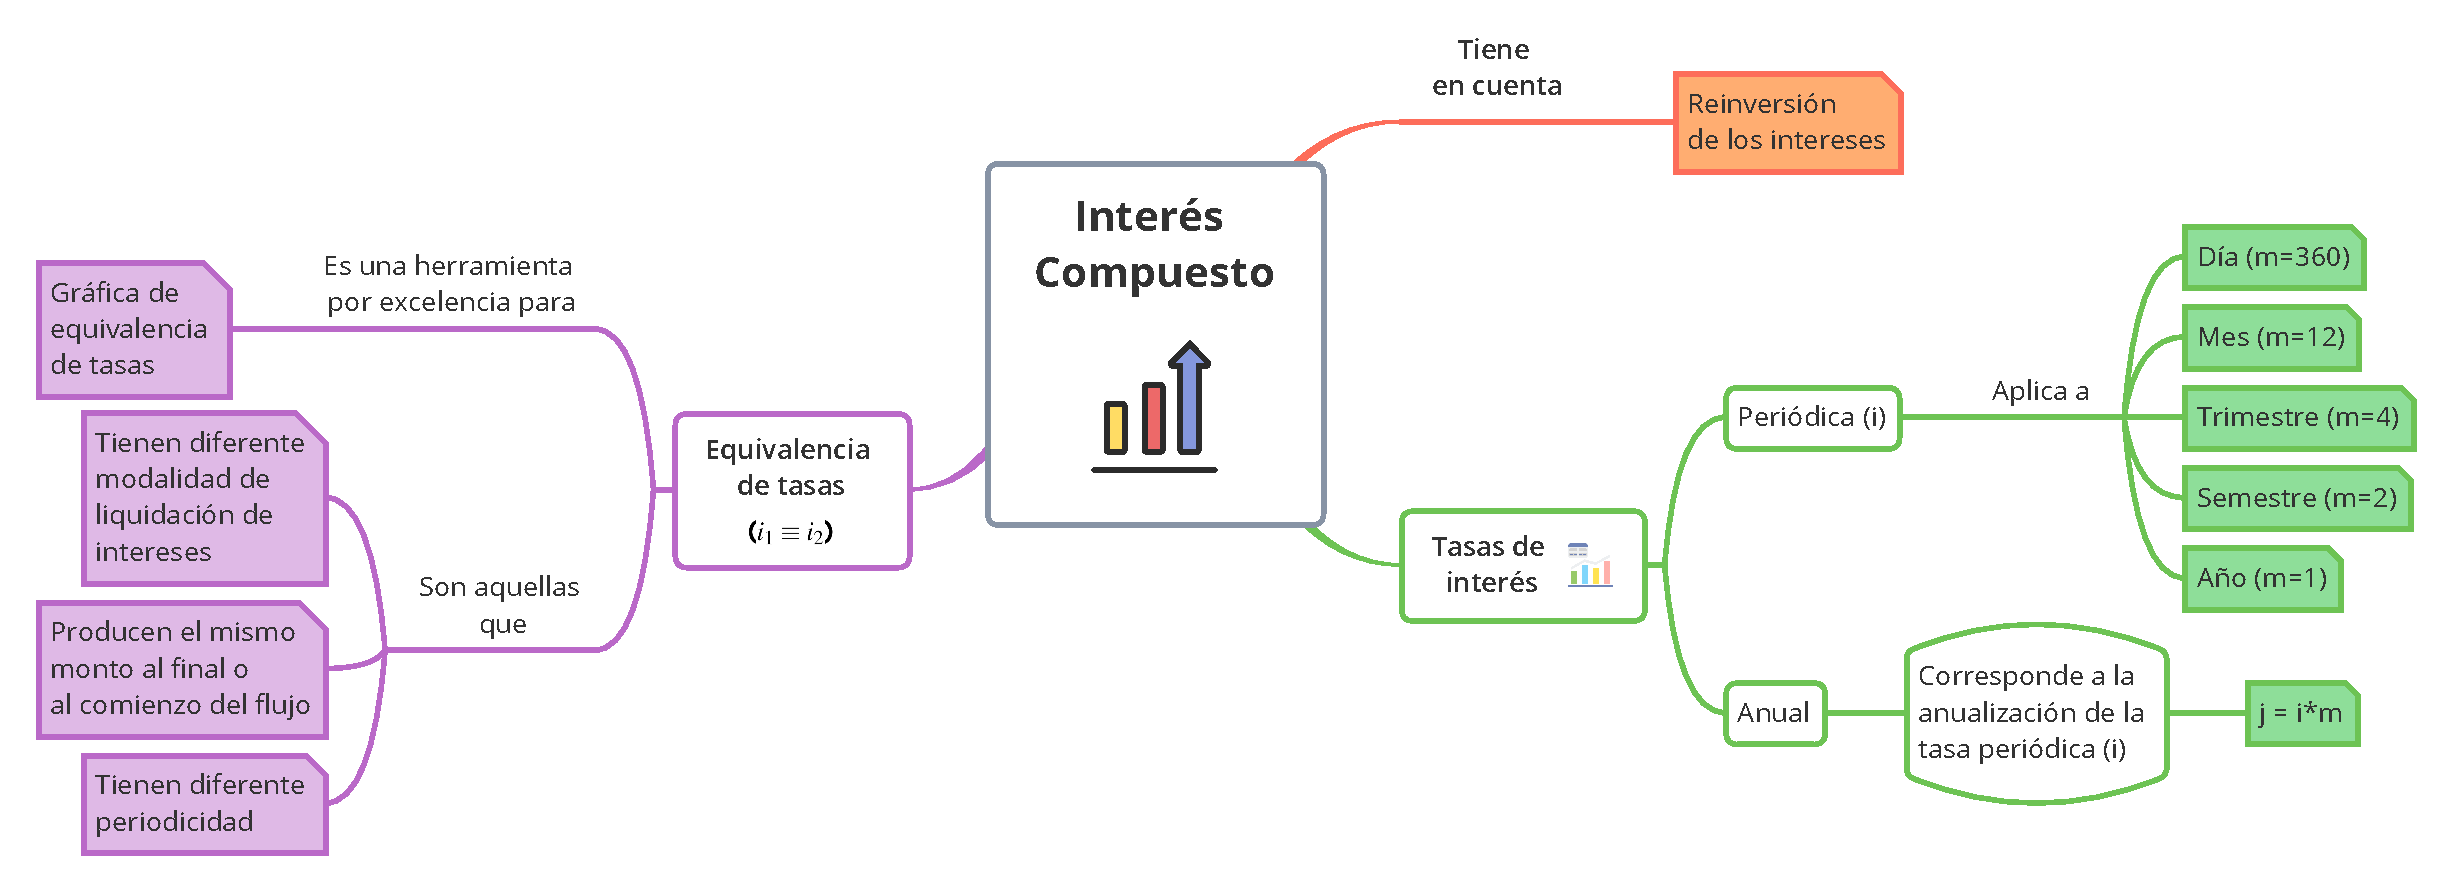
\includegraphics[height = 5.6 cm]{Mapa Mental 2.1.pdf}\\
\end{center}
\clearpage
\section{{Fórmulas del Capítulo}}
\begin{spacing}{1.3}
   \begin{center}
      \begin{tabular}{ |p{4cm}|p{5cm}| p{5cm}|}
         \hline
         \rowcolor{orange!50}
         \begin{center}\textbf{Fórmula} \end{center}   & \begin{center} \textbf{Nombre}\end{center} & \begin{center} \textbf{Excel} \end{center} \\ \hline
         F = $P(1+i)^n$                                & Valor futuro                               & VF(i;n;;VA,0)                              \\ \hline
         P = $\frac{F}{(1 + i)^{n}}$                   & Valor presente                             & VA(i;n;;VF,0)                              \\ \hline
         j = i(m)                                      & Tasa periódica anualizada                  & TASA.NOMINAL(i;m)                          \\ \hline
         ${(1 + i_{1})^{m_1}}$ = ${(1 + i_{2})^{m_2}}$ & Equivalencia de tasas                      & TASA(m;;-1;1+i)                            \\ \hline
      \end{tabular}
   \end{center}
\end{spacing}
\section{Interés compuesto}
Es la acumulación de intereses producidos por un capital inicial a una tasa de interés durante períodos determinados.\\

% ejemplo1
\textbf{Ejemplo 1:}\\
Tenemos un capital de 200{.}000 COP que será invertido al 10\% 
periódico trimestre vencido (ptv), durante un año. Use año de 360 días.\\

A. Calcular el valor total de los intereses simples, si:
\begin{itemize}
  \item son cancelados cada trimestre.
  \item son capitalizados y cancelados al final del tiempo de la inversión.
\end{itemize}
B. ¿A qué tasa de interés periódica año vencido (pav) es equivalente la tasa de 10\% 
periódica trimestre vencido (ptv)?\\

%%%%%%%%%%%%%%%%%%% EJERCICIO 1 %%%%%%

%\newpage %USAR SOLO SI EL SOLUCIÓN QUEDA SOLO Y ES NECESARIO BAJARLO A LA SIGUIENTE PAGINA
\textbf{Solución.}\\

%La tabla ira centrada
\begin{center}
  \renewcommand{\arraystretch}{1.5}% Margenes de las celdas
  %Creación de la cuadricula de 3 columnas
  \begin{flushleft}\textbf{A.1} \end{flushleft}
  \begin{longtable}[H]{|C{0.3\linewidth}|C{0.3\linewidth}|C{0.3\linewidth}|}
    %Creamos una linea horizontal
    \hline
    %Definimos el color de la primera fila
    \rowcolor[HTML]{FFB183}
    %%%%% INICIO ASIGNACIÓN PERIODO FOCAL %%%%%%%
    %%%%%%%%%% INICIO TITULO
    %Lo que se hace aquí es mezclar las 3 columnas en una sola
    \multicolumn{3}{|c|}{\cellcolor[HTML]{FFB183}\textbf{1. Asignación período focal}} \\ \hline
    %%%%%%%%%% FIN TITULO
    %%%%% INICIO DECLARACIÓN DE VARIABLES %%%%%%%
    \multicolumn{3}{|c|}{$pf = 4ptv$}  \\ \hline
    %%%%%%%%%% INICIO TITULO
    %Lo que se hace aquí es mezclar las 3 columnas en una sola
    \multicolumn{3}{|c|}{\cellcolor[HTML]{FFB183}\textbf{2. Declaración de variables}}  \\ \hline
    %%%%%%%%%% FIN TITULO
    %%%%%%%%%% INICIO DE MATEMÁTICAS
    %Cada & hace referencia al paso de la siguiente columna
    $P =  200{.}000 COP$ & $i = 10\%\textit{ ptv} $  & $I= ? COP$  \\
      & $n=\frac{90 dias}{90dias} =1 ptv$  & $F= ? COP$
    \\\hline

    %%%%%%%%%% FIN DE MATEMÁTICAS
    %%%%% FIN DECLARACIÓN DE VARIABLES


    %%%%% INICIO FLUJO DE CAJA
    \rowcolor[HTML]{FFB183}
    \multicolumn{3}{|c|}{\cellcolor[HTML]{FFB183}\textbf{3. Diagrama de flujo de caja}}  \\ \hline
    %Mezclamos 3 columnas y podremos el dibujo
    %%%%%%%%%%%%% INSERCIÓN DE LA IMAGEN
    %Deberán descargar las imágenes respectivas del drive y pegarlas en la carpeta
    %n_capitulo/img/ejemplos/1/capitulo1ejemplo1.pdf  (el /1/ es el numero del ejemplo)
    \multicolumn{3}{|c|}{ 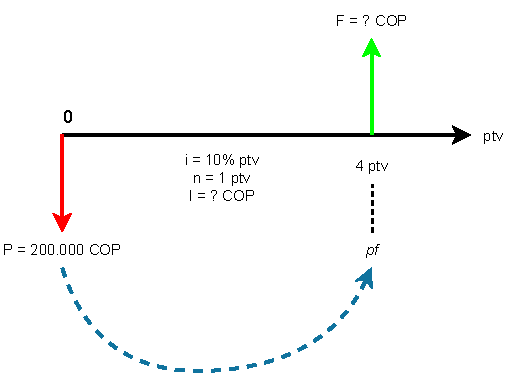
\includegraphics[trim=-5 -5 -5 -5 , scale=1]{2_Capitulo/ejemplos/1/Capitulo2Ejercicio1a_v2.pdf} }  \\ \hline
    %%%%%%%%%%%%% FIN INSERCIÓN DE IMAGEN
    %%%%%FIN FLUJO DE CAJA



    %%%%% INICIO DECLARACIÓN FORMULAS
    %%%%%%%%%%% INICIO TITULO
    \rowcolor[HTML]{FFB183}
    \multicolumn{3}{|c|}{\cellcolor[HTML]{FFB183}\textbf{4. Declaración de fórmulas}}  \\ \hline
    %%%%%%%%%%% FIN TITULO
    %%%%%%%%%%% INICIO MATEMÁTICAS

    $I = Pin\hspace{0.3cm} \textit{Interés monetario simple}$ & \multicolumn{2}{c|}{$F = P + I \hspace{0.3cm} \textit{Valor futuro}$}                 \\ \hline
    %%%%%%%%%% FIN MATEMÁTICAS
    %%%%%% INICIO DESARROLLO MATEMÁTICO
    \rowcolor[HTML]{FFB183}
    %%%%%%%%%%INICIO TITULO
    \multicolumn{3}{|c|}{\cellcolor[HTML]{FFB183}\textbf{5. Desarrollo matemático}}                                                                   \\ \hline
    %%%%%%%%%% FIN TITULO
    %%%%%%%%%% INICIO MATEMÁTICAS
    \multicolumn{3}{|c|}{$I_{1}= (200.000 COP)(0.1)(1)$}                                                                                             \\ \multicolumn{3}{|c|}{$I_{1}=   20{.}000 COP$}  \\ \multicolumn{3}{|c|}{$I_{1} = I_{2} = I_{3} = I_{4}$}  \\
    \multicolumn{3}{|c|}{$I = (4)(20.000 COP) =  80.000 COP$}                                                                                       \\ \multicolumn{3}{|c|}{$F = P + I$} \\ \multicolumn{3}{|c|}{$F = 200{.}000 COP +  80{.}000 COP =  280{.}000 COP$} \\ \hline


    %%%%%%%%%% FIN MATEMÁTICAS
    %%%%%% FIN DESARROLLO MATEMÁTICO
    %%%%%% INICIO RESPUESTA
    \rowcolor[HTML]{FFB183}
    %%%%%%%%%%INICIO TITULO
    \multicolumn{3}{|c|}{\cellcolor[HTML]{FFB183}\textbf{6. Respuesta}}                                                                               \\ \hline
    %%%%%%%%%% FIN TITULO
    %%%%%%%%%% INICIO RESPUESTA MATEMÁTICA
    $I= 80{.}000 COP$                                        &
    \multicolumn{2}{c|}{$F= 280{.}000 COP$
    }                                                                                                                                                 \\ \hline
    %%%%%%%%%% FIN MATEMÁTICA
    %%%%%% FIN RESPUESTA
  \end{longtable}
  %Se crean dos lineas en blanco para que no quede el siguiente texto tan pegado
  %\newline \newline %USARLO SI CREES QUE ES NECESARIO
\end{center}
%%%%%%%%%%%%%%%%%%%%%%%%%%FIN EJERCICIO 1 %%%%%%%%%%%%%%%%%%%%%%%%%%%


\clearpage

En resumen, se tiene en el inciso A:
\begin{table}[htbp]
   \begin{center}
      \begin{tabular}{|l|l|l|l|}
         \hline
         Período & Capital Inicial & Interés     & Capital Final \\
         \hline
         0       & 200.000 COP &  0 COP      & 200.000 COP  \\ \hline
         1       & 200.000 COP &  20.000 COP & 220.000 COP  \\ \hline
         2       & 200.000 COP &  20.000 COP & 240.000 COP  \\ \hline
         3       & 200.000 COP &  20.000 COP & 260.000 COP  \\ \hline
         4       & 200.000 COP &  20.000 COP & 280.000 COP  \\ \hline
      \end{tabular}
      \label{tabla:interesSimple1}
   \end{center}
\end{table}

%%%%%%%%%%%%%%%%%%% EJERCICIO 1 %%%%%%

%\newpage %USAR SOLO SI EL SOLUCIÓN QUEDA SOLO Y ES NECESARIO BAJARLO A LA SIGUIENTE PAGINA

%La tabla ira centrada
\begin{center}
  \renewcommand{\arraystretch}{1.5}% Margenes de las celdas
  %Creación de la cuadricula de 3 columnas
  \begin{flushleft}\textbf{A.2} \end{flushleft}
  \begin{longtable}[H]{|C{0.3\linewidth}|C{0.3\linewidth}|C{0.3\linewidth}|}
    %Creamos una linea horizontal
    \hline
    %Definimos el color de la primera fila
    \rowcolor[HTML]{FFB183}
    %%%%% INICIO ASIGNACIÓN FECHA FOCAL %%%%%%%
    %%%%%%%%%% INICIO TITULO
    %Lo que se hace aquí es mezclar las 3 columnas en una sola
    \multicolumn{3}{|c|}{\cellcolor[HTML]{FFB183}\textbf{1. Asignación período focal}}  \\ \hline
    %%%%%%%%%% FIN TITULO
    %%%%% INICIO DECLARACIÓN DE VARIABLES %%%%%%%
    \multicolumn{3}{|c|}{$pf = 4ptv$} \\ \hline
    %%%%%%%%%% INICIO TITULO
    %Lo que se hace aquí es mezclar las 3 columnas en una sola
    \multicolumn{3}{|c|}{\cellcolor[HTML]{FFB183}\textbf{2. Declaración de variables}}  \\ \hline
    %%%%%%%%%% FIN TITULO
    %%%%%%%%%% INICIO DE MATEMÁTICAS
    %Cada & hace referencia al paso de la siguiente columna
    
    $P =  200{.}000 COP$  & $i = 10\%\textit{ ptv} $  & $I= ? COP$   \\
      & $n=\frac{360 \textit{días}}{90 \textit{días}} =4 ptv$ & $F= ? COP$
    \\\hline

    %%%%%%%%%% FIN DE MATEMÁTICAS
    %%%%% FIN DECLARACIÓN DE VARIABLES

    %%%%% INICIO FLUJO DE CAJA
    \rowcolor[HTML]{FFB183}
    \multicolumn{3}{|c|}{\cellcolor[HTML]{FFB183}\textbf{3. Diagrama de flujo de caja}}                                                                          \\ \hline
    %Mezclamos 3 columnas y pondremos el dibujo
    %%%%%%%%%%%%% INSERCIÓN DE LA IMAGEN
    %Deberán descargar las imágenes respectivas del drive y pegarlas en la carpeta
    %n_capitulo/img/ejemplos/1/capitulo1ejemplo1.pdf  (el /1/ es el numero del ejemplo)
    \multicolumn{3}{|c|}{ 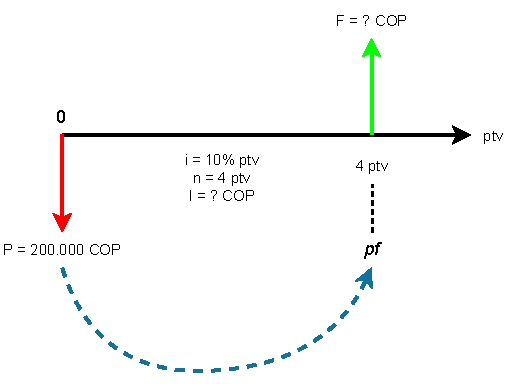
\includegraphics[trim=-5 -5 -5 -5 , scale=1]{2_Capitulo/ejemplos/1/Capitulo2Ejercicio1a2_v2.pdf} }                                         \\ \hline
    %%%%%%%%%%%%% FIN INSERCIÓN DE IMAGEN
    %%%%%FIN FLUJO DE CAJA

    %%%%% INICIO DECLARACIÓN FORMULAS
    %%%%%%%%%%% INICIO TITULO
    \rowcolor[HTML]{FFB183}
    \multicolumn{3}{|c|}{\cellcolor[HTML]{FFB183}\textbf{4. Declaración de fórmulas}}                                                                            \\ \hline
    %%%%%%%%%%% FIN TITULO
    %%%%%%%%%%% INICIO MATEMÁTICAS

    $I = Pin\hspace{0.3cm} \textit{Interés monetario simple}$ & \multicolumn{2}{c|}{$F = P + I \hspace{0.3cm} \textit{Valor futuro}$}                            \\ \hline
    %%%%%%%%%% FIN MATEMÁTICAS
    %%%%%% INICIO DESARROLLO MATEMÁTICO
    \rowcolor[HTML]{FFB183}
    %%%%%%%%%%INICIO TITULO
    \multicolumn{3}{|c|}{\cellcolor[HTML]{FFB183}\textbf{5. Desarrollo matemático}}                                                                              \\ \hline
    %%%%%%%%%% FIN TITULO
    %%%%%%%%%% INICIO MATEMÁTICAS
    $n=4ptv$                                                  & \multicolumn{2}{c|}{}                                                                            \\ $I_{1}= 200{.}000$ COP$\cdot0.1\cdot1$ & \multicolumn{2}{c|}{$F =  200{.}000$ COP + $20{.}000$ COP + $22{.}000$ COP}  \\ $I_{1}=  20{.}000$ COP & \multicolumn{2}{c|}{$+ 24{.}200$ COP + $26{.}620$ COP}  \\
    $I_{2}= 220{.}000\cdot0.1\cdot1$ COP   & \multicolumn{2}{c|}{$F= P+I$} \\
    $I_{2}= 22{.}000$ COP                  & \multicolumn{2}{c|}{$F=200{.}000$ COP$+92{.}820$ COP}   \\
    $I_{3}= 242{.}000\cdot0.1\cdot1$ COP   & \multicolumn{2}{c|}{$F= 292{.}820$ COP}                \\
    $I_{3}= 24{.}200$ COP                  & \multicolumn{2}{c|}{}                                                           \\
    $I_{4}= 266{.}200\cdot0.1\cdot1$ COP   & \multicolumn{2}{c|}{}                                                                            \\
    $I_{4}= 26{.}620$ COP                  & \multicolumn{2}{c|}{}                                                                            \\
    $I= 20{.}000 COP + 22{.}000 COP + 24{.}200 COP + 26{.}620 COP$& \multicolumn{2}{c|}{}                                        \\
    $I= 92{.}820$ COP                      & \multicolumn{2}{c|}{}
    
    \\ \hline
    %%%%%%%%%% FIN MATEMÁTICAS
    %%%%%% FIN DESARROLLO MATEMÁTICO
    %%%%%% INICIO RESPUESTA
    \rowcolor[HTML]{FFB183}
    %%%%%%%%%%INICIO TITULO
    \multicolumn{3}{|c|}{\cellcolor[HTML]{FFB183}\textbf{6. Respuesta}}                                                                                          \\ \hline
    %%%%%%%%%% FIN TITULO
    %%%%%%%%%% INICIO RESPUESTA MATEMÁTICA
    $I= 92{.}820 COP$                                         &
    \multicolumn{2}{c|}{$F= 292{.}820 COP$
    }                                                                                                                                                            \\ \hline
    %%%%%%%%%% FIN MATEMÁTICAS
    %%%%%% FIN RESPUESTA
  \end{longtable}
  %Se crean dos lineas en blanco para que no quede el siguiente texto tan pegado
  %\newline \newline %USARLO SI CREES QUE ES NECESARIO
\end{center}
%%%%%%%%%%%%%%%%%%%%%%%%%%FIN EJERCICIO 1 %%%%%%%%%%%%%%%%%%%%%%%%%%%



Representando en una tabla la información obtenida en el apartado anterior del ejercicio se tiene lo siguiente:\\

\begin{table}[htbp]
   \begin{center}
      \begin{tabular}{|l|l|l|l|}
         \hline
         Período & Capital Inicial & Interés     & Capital Final \\
         \hline
         0 & 200.000 COP & 0 COP      & 200.000 COP \\ \hline
         1 & 200.000 COP & 20.000 COP & 220.000 COP \\ \hline
         2 & 220.000 COP & 22.000 COP & 242.000 COP \\ \hline
         3 & 242.000 COP & 24.200 COP & 266.000 COP \\ \hline
         4 & 266.000 COP & 26.000 COP & 292.000 COP \\ \hline
      \end{tabular}
      \label{tabla:interesCompuesto1}
   \end{center}
\end{table}
\textbf{Generalizando:}\\
\begin{table}[htbp]
   \begin{center}
      \begin{tabular}{|l|l|l|l|}
         \hline
         Período & Capital Inicial & Interés         & Capital Final                                       \\
         \hline
         0       & P               & 0               & $F_{0}$=P                                           \\ \hline
         1       & P               & Pi              & $F_{1}$ = P + Pi = P(1+i)                           \\ \hline
         2       & P(1+i)          & P(1+i)i         & $F_{2}$ = P(1+i) + P(1+i)i = $P(1+i)^{2}$           \\ \hline
         .       & .               & .               & .                                                   \\ \hline
         ..      & ..              & ..              & ..                                                  \\ \hline
         ...     & ...             & ...             & ...                                                 \\ \hline
         n       & $P(1+i)^{n-1}$  & $P(1+i)^{n-1}i$ & $F_{n} = P(1+i)^{n-1} + P(1+i)^{n-1}i = P(1+i)^{n}$ \\ \hline
      \end{tabular}
      \label{tabla:interesCompuesto2}
   \end{center}
\end{table}

Se concluye que la fórmula del interés compuesto es:\\
$F = P(1+i)^n$ \hspace{20 pt} \textit{Valor futuro}\\

\textbf{Volviendo al ejemplo 1:}\\
$F = P(1+i)^n$\\
$F =  200.000 (1+0,1)^4$ COP\\
$F =  292.820$ COP\\

%%%%%%%%%%%%%%%%%%% EJERCICIO 1 %%%%%%

\newpage %USAR SOLO SI EL SOLUCIÓN QUEDA SOLO Y ES NECESARIO BAJARLO A LA SIGUIENTE PAGINA

%La tabla ira centrada
\begin{center}
	\renewcommand{\arraystretch}{1.5}% Margenes de las celdas
	%Creación de la cuadricula de 3 columnas
	\begin{flushleft}\textbf{B} \end{flushleft}
	\begin{longtable}[H]{|C{0.3\linewidth}|C{0.3\linewidth}|C{0.3\linewidth}|}
		%Creamos una linea horizontal
		\hline
		%Definimos el color de la primera fila
		\rowcolor[HTML]{FFB183}
		%%%%% INICIO ASIGNACIÓN FECHA FOCAL %%%%%%%
		%%%%%%%%%% INICIO TITULO
		%Lo que se hace aquí es mezclar las 3 columnas en una sola
		\multicolumn{3}{|c|}{\cellcolor[HTML]{FFB183}\textbf{1. Asignación período focal}}   \\ \hline
		%%%%%%%%%% FIN TITULO
		%%%%% INICIO DECLARACIÓN DE VARIABLES %%%%%%%
		\multicolumn{3}{|c|}{$pf = 1pav$} \\ \hline
		%%%%%%%%%% INICIO TITULO
		%Lo que se hace aquí es mezclar las 3 columnas en una sola
		\multicolumn{3}{|c|}{\cellcolor[HTML]{FFB183}\textbf{2. Declaración de variables}}   \\ \hline
		%%%%%%%%%% FIN TITULO
		%%%%%%%%%% INICIO DE MATEMÁTICAS
		%Cada & hace referencia al paso de la siguiente columna
		$P =  200{.}000 COP$   													& $i_{1} = 10\%\textit{ptv} $  		& $i_{2}=?\%pav$    							\\

		$F= 292{.}820 COP$ & $n=\frac{360 \textit{días}}{360 \textit{días}} =1 pav$   		&
		\\\hline

		%%%%%%%%%% FIN DE MATEMÁTICAS
		%%%%% FIN DECLARACIÓN DE VARIABLES


		%%%%% INICIO FLUJO DE CAJA
		\rowcolor[HTML]{FFB183}
		\multicolumn{3}{|c|}{\cellcolor[HTML]{FFB183}\textbf{3. Diagrama de flujo de caja}} \\ \hline
		%Mezclamos 3 columnas y pondremos el dibujo
		%%%%%%%%%%%%% INSERCIÓN DE LA IMAGEN
		%Deberán descargar las imágenes respectivas del drive y pegarlas en la carpeta
		%n_capitulo/img/ejemplos/1/capitulo1ejemplo1.pdf  (el /1/ es el numero del ejemplo)
		\multicolumn{3}{|c|}{ 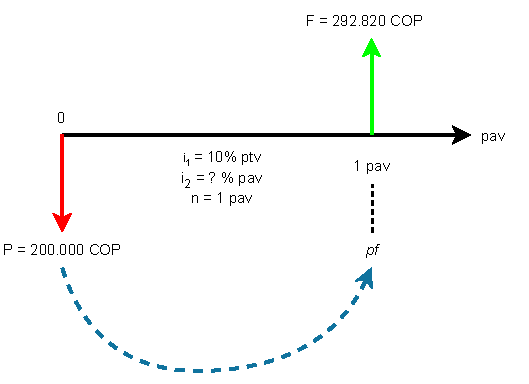
\includegraphics[trim=-5 -5 -5 -5 , scale=1]{2_Capitulo/ejemplos/1/Capitulo2Ejercicio1b_v2.pdf} }   \\ \hline
		%%%%%%%%%%%%% FIN INSERCIÓN DE IMAGEN
		%%%%%FIN FLUJO DE CAJA



		%%%%% INICIO DECLARACIÓN FORMULAS
		%%%%%%%%%%% INICIO TITULO
		\rowcolor[HTML]{FFB183}
		\multicolumn{3}{|c|}{\cellcolor[HTML]{FFB183}\textbf{4. Declaración de fórmulas}}    \\ \hline
		%%%%%%%%%%% FIN TITULO
		%%%%%%%%%%% INICIO MATEMÁTICAS

		\multicolumn{3}{|c|}{$F = P(1+i)^n \hspace{0.3cm} \textit{Valor futuro}$} \\ \hline
		%%%%%%%%%% FIN MATEMÁTICAS
		%%%%%% INICIO DESARROLLO MATEMÁTICO
		\rowcolor[HTML]{FFB183}
		%%%%%%%%%%INICIO TITULO
		\multicolumn{3}{|c|}{\cellcolor[HTML]{FFB183}\textbf{5. Desarrollo matemático}}       \\ \hline
		%%%%%%%%%% FIN TITULO
		%%%%%%%%%% INICIO MATEMÁTICAS
		\multicolumn{3}{|c|}{$ 292{.}820 COP= 200{.}000 COP(1+i_{2})^1$} \\
		\multicolumn{3}{|c|}{$\frac{ 292{.}820 COP}{ 200{.}000 COP}=1+i_{2}$} \\
        \multicolumn{3}{|c|}{$\frac{ 292{.}820 COP}{ 200{.}000 COP}-1=i_{2}$} \\
		\multicolumn{3}{|c|}{$i_{2}=0.4641\equiv46.41\%pav$}
		\\ \hline
		%%%%%%%%%% FIN MATEMÁTICAS
		%%%%%% FIN DESARROLLO MATEMÁTICO
		%%%%%% INICIO RESPUESTA
		\rowcolor[HTML]{FFB183}
		%%%%%%%%%%INICIO TITULO
		\multicolumn{3}{|c|}{\cellcolor[HTML]{FFB183}\textbf{6. Respuesta}}   \\ \hline
		%%%%%%%%%% FIN TITULO
		%%%%%%%%%% INICIO RESPUESTA MATEMÁTICA
		\multicolumn{3}{|c|}{$i_{2}=46.41\%pav$}  \\ \hline
		%%%%%%%%%% FIN MATEMÁTICAS
		%%%%%% FIN RESPUESTA
	\end{longtable}
	%Se crean dos lineas en blanco para que no quede el siguiente texto tan pegado
	%\newline \newline %USARLO SI CREES QUE ES NECESARIO
\end{center}
%%%%%%%%%%%%%%%%%%%%%%%%%%FIN EJERCICIO 1 %%%%%%%%%%%%%%%%%%%%%%%%%%%


\section{Tasa de interés nominal anual (j)}
Corresponde a la anualización de la tasa periódica (i):\\
$j = i(m)$\\
\textbf{Ejemplo 2}\\
Se invierten 200{.}000 COP en un depósito a término fijo de 6 meses en un banco que paga el 28\% namv. Determinar el monto de la entrega al vencimiento.\\

%%%%%%%%%%%%%%%%%%% EJERCICIO 1 %%%%%%

%\newpage %USAR SOLO SI EL SOLUCIÓN QUEDA SOLO Y ES NECESARIO BAJARLO A LA SIGUIENTE PAGINA
\textbf{Solución.}
%La tabla ira centrada
\begin{center}
  \renewcommand{\arraystretch}{1.5}% Margenes de las celdas
  %Creación de la cuadricula de 3 columnas \end{flushleft}
  \begin{longtable}[H]{|C{0.3\linewidth}|C{0.3\linewidth}|C{0.3\linewidth}|}
    %Creamos una linea horizontal
    \hline
    %Definimos el color de la primera fila
    \rowcolor[HTML]{FFB183}
    %%%%% INICIO ASIGNACIÓN FECHA FOCAL %%%%%%%
    %%%%%%%%%% INICIO TITULO
    %Lo que se hace aquí es mezclar las 3 columnas en una sola
    \multicolumn{3}{|c|}{\cellcolor[HTML]{FFB183}\textbf{1. Asignación período focal}}                                  \\ \hline
    %%%%%%%%%% FIN TITULO
    %%%%% INICIO DECLARACIÓN DE VARIABLES %%%%%%%
    \multicolumn{3}{|c|}{$pf = 6pmv$}                                                                                   \\ \hline
    %%%%%%%%%% INICIO TITULO
    %Lo que se hace aquí es mezclar las 3 columnas en una sola
    \multicolumn{3}{|c|}{\cellcolor[HTML]{FFB183}\textbf{2. Declaración de variables}}                                  \\ \hline
    %%%%%%%%%% FIN TITULO
    %%%%%%%%%% INICIO DE MATEMÁTICAS
    %Cada & hace referencia al paso de la siguiente columna
    $P =  200{.}000$ COP & $n = 6\textit{pmv} $ & $i= ?\% pmv$                                                           \\
    $j=28\%namv$         & $m=12pmv$            & $F = ? COP$                                                           
    \\\hline

    %%%%%%%%%% FIN DE MATEMÁTICAS
    %%%%% FIN DECLARACIÓN DE VARIABLES


    %%%%% INICIO FLUJO DE CAJA
    \rowcolor[HTML]{FFB183}
    \multicolumn{3}{|c|}{\cellcolor[HTML]{FFB183}\textbf{3. Diagrama de flujo de caja}}                                 \\ \hline
    %Mezclamos 3 columnas y pondremos el dibujo
    %%%%%%%%%%%%% INSERCIÓN DE LA IMAGEN
    %Deberán descargar las imágenes respectivas del drive y pegarlas en la carpeta
    %n_capitulo/img/ejemplos/1/capitulo1ejemplo1.pdf  (el /1/ es el numero del ejemplo)
    \multicolumn{3}{|c|}{ 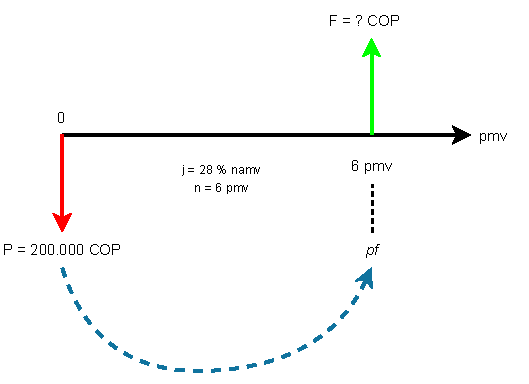
\includegraphics[trim=-5 -5 -5 -5 , scale=1]{2_Capitulo/ejemplos/2/Capitulo2Ejercicio2_v2.pdf} } \\ \hline
    %%%%%%%%%%%%% FIN INSERCIÓN DE IMAGEN
    %%%%%FIN FLUJO DE CAJA



    %%%%% INICIO DECLARACIÓN FORMULAS
    %%%%%%%%%%% INICIO TITULO
    \rowcolor[HTML]{FFB183}
    \multicolumn{3}{|c|}{\cellcolor[HTML]{FFB183}\textbf{4. Declaración de fórmulas}}                                   \\ \hline
    %%%%%%%%%%% FIN TITULO
    %%%%%%%%%%% INICIO MATEMÁTICAS
    \multicolumn{3}{|c|}{$F = P(1+i)^n \hspace{0.3cm} \textit{Valor futuro}$}                                           \\
    \multicolumn{3}{|c|}{$j=i\cdot m\hspace{0.3cm}\textit{Tasa periódica anualizada}$}
    \\ \hline
    %%%%%%%%%% FIN MATEMÁTICAS
    %%%%%% INICIO DESARROLLO MATEMÁTICO
    \rowcolor[HTML]{FFB183}
    %%%%%%%%%%INICIO TITULO
    \multicolumn{3}{|c|}{\cellcolor[HTML]{FFB183}\textbf{5. Desarrollo matemático}}                                     \\ \hline
    %%%%%%%%%% FIN TITULO
    %%%%%%%%%% INICIO MATEMÁTICAS
    \multicolumn{3}{|c|}{$0{.}28=i\cdot 12$}                                                                            \\
    \multicolumn{3}{|c|}{$i= \frac{0{.}28}{12} = 0{.}02333... \equiv 2{.}333\%pmv$}                                     \\
    \multicolumn{3}{|c|}{$0{.}28=i\cdot 12$}                                                                            \\
    \multicolumn{3}{|c|}{$F = 200{.}000 COP(1+0,2333)^6$}                                                       \\
    \multicolumn{3}{|c|}{$F = 229{.}685.04 COP$}
    \\ \hline


    %%%%%%%%%% FIN MATEMÁTICAS
    %%%%%% FIN DESARROLLO MATEMÁTICO
    %%%%%% INICIO RESPUESTA
    \rowcolor[HTML]{FFB183}
    %%%%%%%%%%INICIO TITULO
    \multicolumn{3}{|c|}{\cellcolor[HTML]{FFB183}\textbf{6. Respuesta}}                                                 \\ \hline
    %%%%%%%%%% FIN TITULO
    %%%%%%%%%% INICIO RESPUESTA MATEMÁTICA
    \multicolumn{3}{|c|}{$F = 229{.}685.04 COP$
    }                                                                                                                   \\ \hline
    %%%%%%%%%% FIN MATEMÁTICAS
    %%%%%% FIN RESPUESTA
  \end{longtable}
  %Se crean dos lineas en blanco para que no quede el siguiente texto tan pegado
  %\newline \newline %USARLO SI CREES QUE ES NECESARIO
\end{center}
%%%%%%%%%%%%%%%%%%%%%%%%%%FIN EJERCICIO 1 %%%%%%%%%%%%%%%%%%%%%%%%%%%

\textbf{Ejemplo 3}\\
Una persona debe cancelar la suma de 2{.}000{.}000 COP al cabo de 18 meses. ¿Cuál debe ser el valor del ahorro que debe hacer hoy en una cuenta que paga el equivalente al 24\% nominal anual trimestre vencido (natv) para poder cancelar la deuda?\\

%%%%%%%%%%%%%%%%%%% EJERCICIO 1 %%%%%%

%\newpage %USAR SOLO SI EL SOLUCIÓN QUEDA SOLO Y ES NECESARIO BAJARLO A LA SIGUIENTE PAGINA
\textbf{Solución.}\\
%La tabla ira centrada
\begin{center}
  \renewcommand{\arraystretch}{1.5}% Margenes de las celdas
  %Creación de la cuadricula de 3 columnas \end{flushleft}
  \begin{longtable}[H]{|C{0.3\linewidth}|C{0.3\linewidth}|C{0.3\linewidth}|}
    %Creamos una linea horizontal
    \hline
    %Definimos el color de la primera fila
    \rowcolor[HTML]{FFB183}
    %%%%% INICIO ASIGNACIÓN FECHA FOCAL %%%%%%%
    %%%%%%%%%% INICIO TITULO
    %Lo que se hace aquí es mezclar las 3 columnas en una sola
    \multicolumn{3}{|c|}{\cellcolor[HTML]{FFB183}\textbf{1. Asignación período focal}}                                  \\ \hline
    %%%%%%%%%% FIN TITULO
    %%%%% INICIO DECLARACIÓN DE VARIABLES %%%%%%%
    \multicolumn{3}{|c|}{$pf = 0ptv$}                                                                                   \\ \hline
    %%%%%%%%%% INICIO TITULO
    %Lo que se hace aquí es mezclar las 3 columnas en una sola
    \multicolumn{3}{|c|}{\cellcolor[HTML]{FFB183}\textbf{2. Declaración de variables}}                                  \\ \hline
    %%%%%%%%%% FIN TITULO
    %%%%%%%%%% INICIO DE MATEMÁTICAS
    %Cada & hace referencia al paso de la siguiente columna
    $F =   2{.}000{.}000$ COP & $j=24\%natv$                     & $P= ?$ COP                                        \\
                               & $i=\frac{24\%natv}{4ptv}=6\%ptv$ &                                                     \\ & $n=\frac{18pmv}{3pmv}=6ptv$ &
    \\\hline

    %%%%%%%%%% FIN DE MATEMÁTICAS
    %%%%% FIN DECLARACIÓN DE VARIABLES


    %%%%% INICIO FLUJO DE CAJA
    \rowcolor[HTML]{FFB183}
    \multicolumn{3}{|c|}{\cellcolor[HTML]{FFB183}\textbf{3. Diagrama de flujo de caja}}                                 \\ \hline
    %Mezclamos 3 columnas y pondremos el dibujo
    %%%%%%%%%%%%% INSERCIÓN DE LA IMAGEN
    %Deberán descargar las imágenes respectivas del drive y pegarlas en la carpeta
    %n_capitulo/img/ejemplos/1/capitulo1ejemplo1.pdf  (el /1/ es el numero del ejemplo)
    \multicolumn{3}{|c|}{ 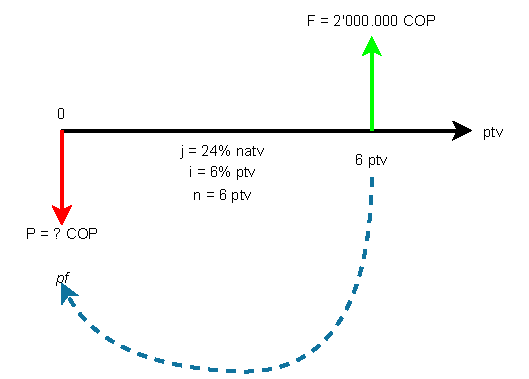
\includegraphics[trim=-5 -5 -5 -5 , scale=1]{2_Capitulo/ejemplos/3/Capitulo2Ejercicio3_v2.pdf} } \\ \hline
    %%%%%%%%%%%%% FIN INSERCIÓN DE IMAGEN
    %%%%%FIN FLUJO DE CAJA



    %%%%% INICIO DECLARACIÓN FORMULAS
    %%%%%%%%%%% INICIO TITULO
    \rowcolor[HTML]{FFB183}
    \multicolumn{3}{|c|}{\cellcolor[HTML]{FFB183}\textbf{4. Declaración de fórmulas}}                                   \\ \hline
    %%%%%%%%%%% FIN TITULO
    %%%%%%%%%%% INICIO MATEMÁTICAS
    \multicolumn{3}{|c|}{$F= P(1+i)^n\hspace{0.3cm} \textit{Valor futuro}$}                                             \\
    \multicolumn{3}{|c|}{$P= F(1+i)^{-n}\hspace{0.3cm} \textit{Valor presente}$}
    \\ \hline
    %%%%%%%%%% FIN MATEMÁTICAS
    %%%%%% INICIO DESARROLLO MATEMÁTICO
    \rowcolor[HTML]{FFB183}
    %%%%%%%%%%INICIO TITULO
    \multicolumn{3}{|c|}{\cellcolor[HTML]{FFB183}\textbf{5. Desarrollo matemático}}                                     \\ \hline
    %%%%%%%%%% FIN TITULO
    %%%%%%%%%% INICIO MATEMÁTICAS
    \multicolumn{3}{|c|}{$P=\frac{2{.}000{.}000 COP}{(1+0.06)^6}$}                                                   \\
    \multicolumn{3}{|c|}{$P=  1{.}409{.}920$ COP}
    \\ \hline


    %%%%%%%%%% FIN MATEMÁTICAS
    %%%%%% FIN DESARROLLO MATEMÁTICO
    %%%%%% INICIO RESPUESTA
    \rowcolor[HTML]{FFB183}
    %%%%%%%%%%INICIO TITULO
    \multicolumn{3}{|c|}{\cellcolor[HTML]{FFB183}\textbf{6. Respuesta}}                                                 \\ \hline
    %%%%%%%%%% FIN TITULO
    %%%%%%%%%% INICIO RESPUESTA MATEMÁTICA
    \multicolumn{3}{|c|}{$P= 1{.}409{.}920$ COP}                                                                   \\ \hline
    %%%%%%%%%% FIN MATEMÁTICAS
    %%%%%% FIN RESPUESTA
  \end{longtable}
  %Se crean dos lineas en blanco para que no quede el siguiente texto tan pegado
  %\newline \newline %USARLO SI CREES QUE ES NECESARIO
\end{center}
%%%%%%%%%%%%%%%%%%%%%%%%%%FIN EJERCICIO 1 %%%%%%%%%%%%%%%%%%%%%%%%%%%


\section{Equivalencia de tasas ($i_{1} \equiv i_{2}$)}
Las tasas equivalentes de interés,  son aquellas que teniendo diferente periodicidad y/o 
modalidad de liquidación de intereses producen el mismo monto al final o al comienzo del flujo.\\
\\
\textbf{Ejemplo 4}\\
¿A que tasa equivalente periódica semestre vencido se debe invertir un capital para que su valor final en un año sea igual al mismo valor invertido en una tasa de 6\% periódico semestre vencido?\\

%%%%%%%%%%%%%%%%%%% EJERCICIO 1 %%%%%%

%\newpage %USAR SOLO SI EL SOLUCIÓN QUEDA SOLO Y ES NECESARIO BAJARLO A LA SIGUIENTE PAGINA
\textbf{Solución.}\\
%La tabla ira centrada
\begin{center}
  \renewcommand{\arraystretch}{1.5}% Margenes de las celdas
  %Creación de la cuadricula de 3 columnas \end{flushleft}
  \begin{longtable}[H]{|C{0.3\linewidth}|C{0.3\linewidth}|C{0.3\linewidth}|}
    %Creamos una linea horizontal
    \hline
    %Definimos el color de la primera fila
    \rowcolor[HTML]{FFB183}
    %%%%% INICIO ASIGNACIÓN FECHA FOCAL %%%%%%%
    %%%%%%%%%% INICIO TITULO
    %Lo que se hace aquí es mezclar las 3 columnas en una sola
    \multicolumn{3}{|c|}{\cellcolor[HTML]{FFB183}\textbf{1. Asignación período focal}}                                    \\ \hline
    %%%%%%%%%% FIN TITULO
    %%%%% INICIO DECLARACIÓN DE VARIABLES %%%%%%%
    \multicolumn{3}{|c|}{$pf = 2psv$}                                                                                     \\ \hline
    %%%%%%%%%% INICIO TITULO
    %Lo que se hace aquí es mezclar las 3 columnas en una sola
    \multicolumn{3}{|c|}{\cellcolor[HTML]{FFB183}\textbf{2. Declaración de variables}}                                    \\ \hline
    %%%%%%%%%% FIN TITULO
    %%%%%%%%%% INICIO DE MATEMÁTICAS
    %Cada & hace referencia al paso de la siguiente columna
    $P =   100{.}000$ COP & $m_{1}=2psv$ & $i_{1}=?\%psv$                                                                \\
                           & $m_{2}=4ptv$ & $i_{2}=6\%ptv$                                                               \\
    \hline

    %%%%%%%%%% FIN DE MATEMÁTICAS
    %%%%% FIN DECLARACIÓN DE VARIABLES


    %%%%% INICIO FLUJO DE CAJA
    \rowcolor[HTML]{FFB183}
    \multicolumn{3}{|c|}{\cellcolor[HTML]{FFB183}\textbf{3. Diagrama de flujo de caja}}                                   \\ \hline
    %Mezclamos 3 columnas y pondremos el dibujo
    %%%%%%%%%%%%% INSERCIÓN DE LA IMAGEN
    %Deberán descargar las imágenes respectivas del drive y pegarlas en la carpeta
    %n_capitulo/img/ejemplos/1/capitulo1ejemplo1.pdf  (el /1/ es el numero del ejemplo)
    \multicolumn{3}{|c|}{ 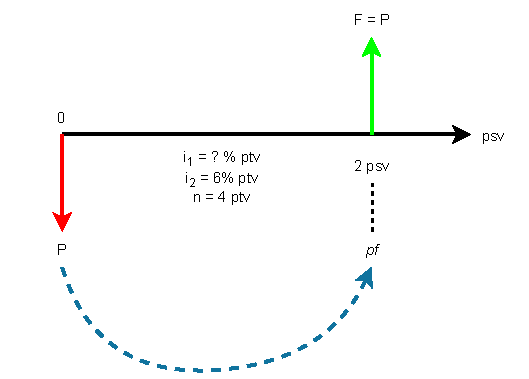
\includegraphics[trim=-5 -5 -5 -5 , scale=1]{2_Capitulo/ejemplos/4/Capitulo2Ejercicio4_v2.pdf} } \\ \hline
    %%%%%%%%%%%%% FIN INSERCIÓN DE IMAGEN
    %%%%%FIN FLUJO DE CAJA



    %%%%% INICIO DECLARACIÓN FORMULAS
    %%%%%%%%%%% INICIO TITULO
    \rowcolor[HTML]{FFB183}
    \multicolumn{3}{|c|}{\cellcolor[HTML]{FFB183}\textbf{4. Declaración de fórmulas}}                                     \\ \hline
    %%%%%%%%%%% FIN TITULO
    %%%%%%%%%%% INICIO MATEMÁTICAS
    \multicolumn{3}{|c|}{$(1+i_{1})^{m_1} = (1+i_{2})^{m_2}\hspace{0.3cm} \textit{Equivalencia de tasas}$}                \\
    \multicolumn{3}{|c|}{$F=P (1+i)^n\hspace{0.3cm} \textit{Valor futuro}$}
    \\ \hline
    %%%%%%%%%% FIN MATEMÁTICAS
    %%%%%% INICIO DESARROLLO MATEMÁTICO
    \rowcolor[HTML]{FFB183}
    %%%%%%%%%%INICIO TITULO
    \multicolumn{3}{|c|}{\cellcolor[HTML]{FFB183}\textbf{5. Desarrollo matemático}}                                       \\ \hline
    %%%%%%%%%% FIN TITULO
    %%%%%%%%%% INICIO MATEMÁTICAS                                                                \\
    \multicolumn{3}{|c|}{$(1+i_{1})^2=(1+0.06)^4$}                                                                         \\
    \multicolumn{3}{|c|}{$i_{1}=0.1236 \equiv 12.36\%psv$}                                                                               \\
    \multicolumn{3}{|c|}{$F=  100{.}000 $COP$ (1+0.06)^4= 126{.}247$ COP}                                                  \\
    \multicolumn{3}{|c|}{$F=  100{.}000 $COP$(1+0.1236)^2=  126{.}247$ COP}
    \\ \hline


    %%%%%%%%%% FIN MATEMÁTICAS
    %%%%%% FIN DESARROLLO MATEMÁTICO
    %%%%%% INICIO RESPUESTA
    \rowcolor[HTML]{FFB183}
    %%%%%%%%%%INICIO TITULO
    \multicolumn{3}{|c|}{\cellcolor[HTML]{FFB183}\textbf{6. Respuesta}}                                                   \\ \hline
    %%%%%%%%%% FIN TITULO
    %%%%%%%%%% INICIO RESPUESTA MATEMÁTICA
    \multicolumn{3}{|c|}{$i_{1}=12.36\%psv$}                                                                                 \\ \hline
    %%%%%%%%%% FIN MATEMÁTICAS
    %%%%%% FIN RESPUESTA
  \end{longtable}
  %Se crean dos lineas en blanco para que no quede el siguiente texto tan pegado
  %\newline \newline %USARLO SI CREES QUE ES NECESARIO
\end{center}
%%%%%%%%%%%%%%%%%%%%%%%%%%FIN EJERCICIO 1 %%%%%%%%%%%%%%%%%%%%%%%%%%%


\section{Relación entre una tasa de interés anticipada(i$_{a}$) y una tasa vencida(i)}
Para $n = 1$, se tiene
$i = \frac{I}{P}$ \\
Si $I = F  d \land P = F (1 -d)$ \hspace{35 pt}\textit{Tasa nominal anual}\\\\
Remplazando en i: \\
$i = \frac {F d} {F (1-d)}$\\\\
Factorizando F,  se obtiene: \\
$i = \frac{d}{(1 - d)}$\\
Remplazando $d = i_{a} $, se obtiene: \\
$i = \frac{ia}{(1 - ia)}$\\\\
Despejando $i_{a}$: \\
$i_{a} = \frac{i}{(1+i)}$ \\\\
$i = \frac{I}{P} = \frac{F d}{F(1-d)}$\\\\
$i = \frac{d}{1-d}$\\

Reemplazando d = $i_{a}$, se obtiene:\\

$i_{a} = \frac{i}{1+i}$\hspace{35 pt}\textit{Tasa periódica anticipada}\\
$j_{a} = i_{a}  (m)$\hspace{23 pt}\textit{Tasa nominal anual anticipada}\\\\

\section{Tasa de interés nominal anual (j) y tasa efectiva anual (EA)}
Según la Superintendencia Financiera de Colombia, la tasa de interés nominal anual es la tasa que el emisor paga al inversionista por un título valor.
Las tasas nominales anuales corresponden a la anualización de una tasa \textbf{periódica}. \\
De igual forma, pueden tener modalidad vencida o anticipada para la liquidación de intereses.\\

\textbf{Tasa de interés efectiva anual (EA):} La tasa de interés efectiva anual, es el instrumento apropiado para medir y comparar, el rendimiento de distintas alternativas de inversión según la Superintendencia Financiera.\\
Según el profesor Javier Serrano, en el libro “Matemáticas financieras y evaluación de proyectos”, la tasa de interés efectiva anual (EA) corresponde a aquella tasa que paga de una sola vez al final del año.\\

Para calcular la tasa efectiva anual, se parte de la fórmula de equivalencia de tasas en donde el
período es anual vencido.

$(1 + i_1)^{m_1} = (1 + i_2)^{m_2}$ , en donde $i_1$ = tasa periódica, que anualizada ($j_1$) es equivalente a la tasa efectiva anual, para un $m_1 = 1 pav$.\\

IMPORTANTE: La tasa Efectiva Anual es equivalente a la tasa Nominal Anual Año Vencido. (naav) \\


\section{Gráfica de equivalencia de tasas}
Gráfica idónea para realizar una equivalencia entre tasas, utilizando las ecuaciones previamente analizadas, se verá que podemos partir de una tasa cualquiera e ir a otra sin necesidad de información adicional.\\
Los puntos que se han colocado del 1 al 8 solo sirven de identificación.\\
\begin{center}
   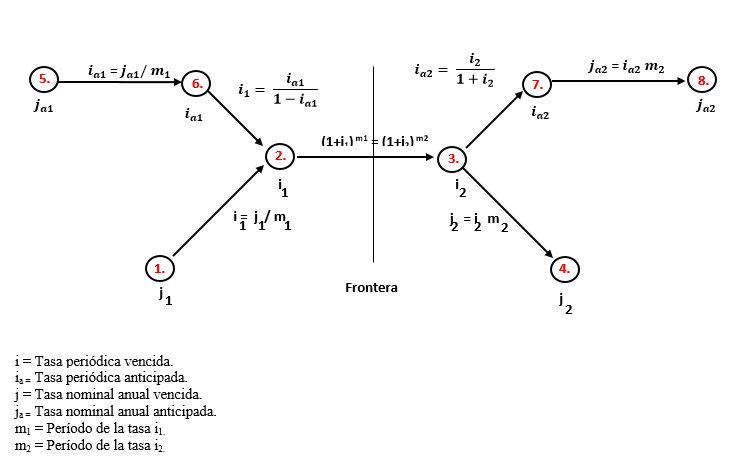
\includegraphics[height = 9.0 cm]{general.png}\\
\end{center}

\textbf{Observación:} Para el uso de la gráfica de equivalencia de tasas, siempre se debe comenzar de un punto de la izquierda y seguir la trayectoria hasta llegar a otro punto situado en la parte derecha.\\
\newpage

\textbf{Ejemplo 5}\\
Dada una tasa del 24\% nominal anual mes vencido, hallar una tasa nominal anual semestre vencido equivalente.\\

%%%%%%%%%%%%%%%%%%% EJERCICIO 1 %%%%%%

%\newpage %USAR SOLO SI EL SOLUCIÓN QUEDA SOLO Y ES NECESARIO BAJARLO A LA SIGUIENTE PAGINA
\textbf{Solución.}\\
%La tabla ira centrada
\begin{center}
  \renewcommand{\arraystretch}{1.5}% Margenes de las celdas
  %Creación de la cuadricula de 3 columnas \end{flushleft}
  \begin{longtable}[H]{|C{0.3\linewidth}|C{0.3\linewidth}|C{0.3\linewidth}|}
    %Creamos una linea horizontal
    \hline
    %%%%%%%%%% INICIO TITULO
    %Lo que se hace aquí es mezclar las 3 columnas en una sola
    \multicolumn{3}{|c|}{\cellcolor[HTML]{FFB183}\textbf{1. Asignación período focal}}                                      \\ \hline
    %%%%%%%%%% FIN TITULO
    %%%%% INICIO DECLARACIÓN DE VARIABLES %%%%%%%
    \multicolumn{3}{|c|}{No aplica}                                                                                         \\ \hline
    %%%%%%%%%% INICIO TITULO
    %Lo que se hace aquí es mezclar las 3 columnas en una sola
    \multicolumn{3}{|c|}{\cellcolor[HTML]{FFB183}\textbf{2. Declaración de variables}}                                      \\ \hline
    %%%%%%%%%% FIN TITULO
    %%%%%%%%%% INICIO DE MATEMÁTICAS
    %Cada & hace referencia al paso de la siguiente columna
    $j_{1}=24\%namv$ & $i_{1}=\frac{24\%namv}{12pmv}=2\%pmv$ & $j_{2}=?\%nasv$                                              \\
    $m_{1}=12pmv$    &                                       &                                                              \\
    $m_{2}=2psv$     &                                       &                                                              \\ \hline

    %%%%%%%%%% FIN DE MATEMÁTICAS
    %%%%% FIN DECLARACIÓN DE VARIABLES


    %%%%% INICIO FLUJO DE CAJA
    \rowcolor[HTML]{FFB183}
    \multicolumn{3}{|c|}{\cellcolor[HTML]{FFB183}\textbf{2. Diagrama de flujo de caja}}                                     \\ \hline
    %Mezclamos 3 columnas y pondremos el dibujo
    %%%%%%%%%%%%% INSERCIÓN DE LA IMAGEN
    %Deberán descargar las imágenes respectivas del drive y pegarlas en la carpeta
    %n_capitulo/img/ejemplos/1/capitulo1ejemplo1.pdf  (el /1/ es el numero del ejemplo)
    \multicolumn{3}{|c|}{ 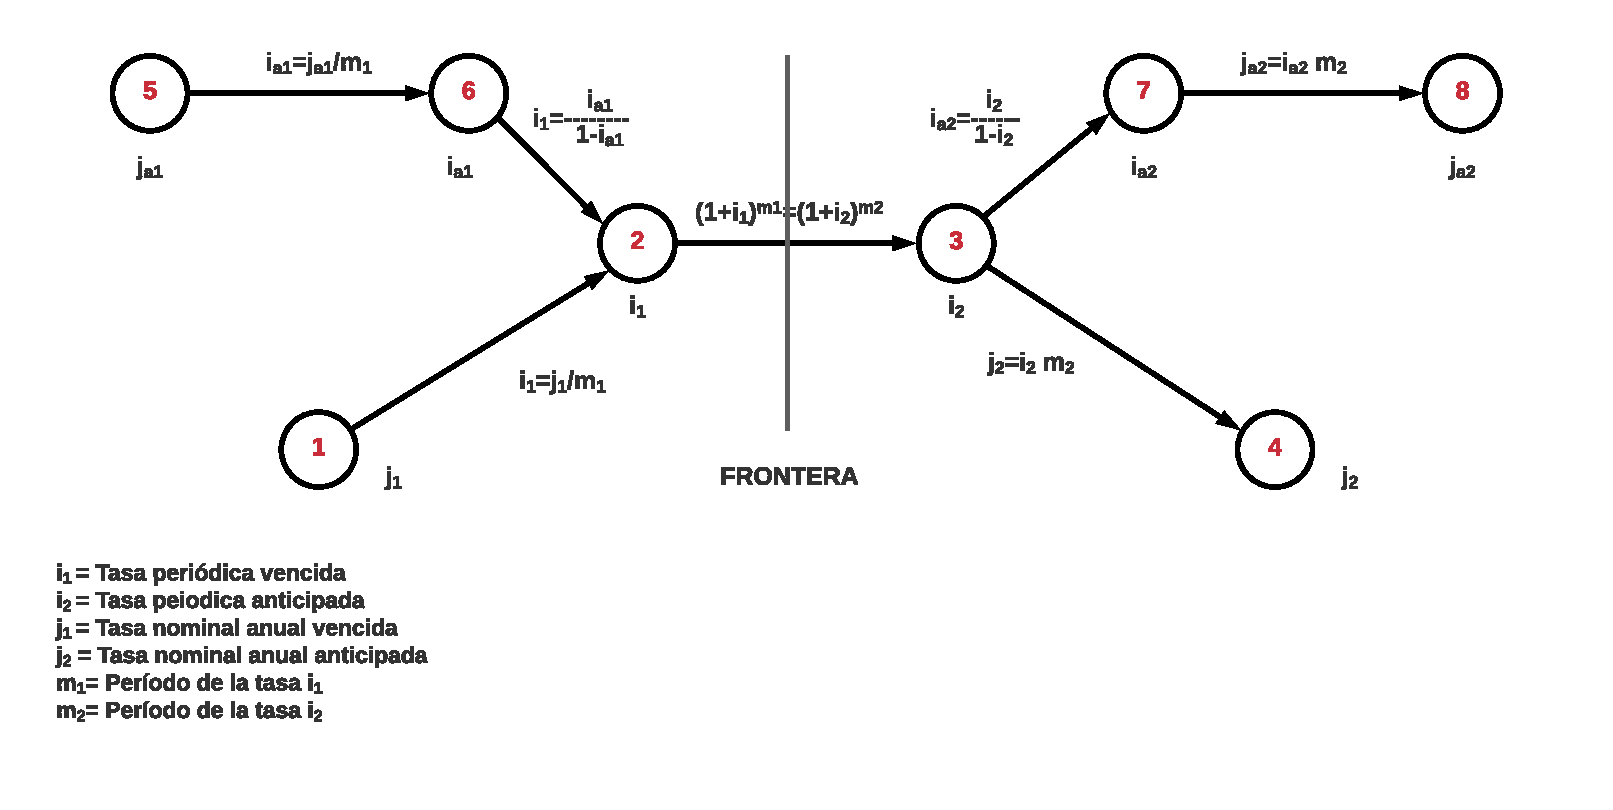
\includegraphics[trim=-5 -5 -5 -5 , scale=0.4]{2_Capitulo/img/ejemplos/6/Capitulo2Ejemplo6.pdf} } \\ \hline
    %%%%%%%%%%%%% FIN INSERCIÓN DE IMAGEN
    %%%%%FIN FLUJO DE CAJA



    %%%%% INICIO DECLARACIÓN FORMULAS
    %%%%%%%%%%% INICIO TITULO
    \rowcolor[HTML]{FFB183}
    \multicolumn{3}{|c|}{\cellcolor[HTML]{FFB183}\textbf{3. Declaración de fórmulas}}                                       \\ \hline
    %%%%%%%%%%% FIN TITULO
    %%%%%%%%%%% INICIO MATEMÁTICAS
    \multicolumn{3}{|c|}{$(1+i_{1})^{m_1} = (1+i_{2})^{m_2}\hspace{0.3cm} \textit{Equivalencia de tasas}$}                  \\
    \multicolumn{3}{|c|}{$j=im\hspace{0.3cm} \textit{Tasa periódica anualizada}$}
    \\ \hline
    %%%%%%%%%% FIN MATEMÁTICAS
    %%%%%% INICIO DESARROLLO MATEMÁTICO
    \rowcolor[HTML]{FFB183}
    %%%%%%%%%%INICIO TITULO
    \multicolumn{3}{|c|}{\cellcolor[HTML]{FFB183}\textbf{4. Desarrollo matemático}}                                         \\ \hline
    %%%%%%%%%% FIN TITULO
    %%%%%%%%%% INICIO MATEMÁTICAS
    \multicolumn{3}{|c|}{$(1+0.02)^{12}=(1+i_{2})^2$}                                                                       \\
    \multicolumn{3}{|c|}{$i_{2}=0.126162 \equiv 12.6162\%psv$}                                                                         \\
    \multicolumn{3}{|c|}{$j_{2}=(12.6162\%psv)(2psv)$}                                                                 \\
    \multicolumn{3}{|c|}{$j_{2}=25.2324\%nasv$}
    \\ \hline


    %%%%%%%%%% FIN MATEMÁTICAS
    %%%%%% FIN DESARROLLO MATEMÁTICO
    %%%%%% INICIO RESPUESTA
    \rowcolor[HTML]{FFB183}
    %%%%%%%%%%INICIO TITULO
    \multicolumn{3}{|c|}{\cellcolor[HTML]{FFB183}\textbf{5. Respuesta}}                                                     \\ \hline
    %%%%%%%%%% FIN TITULO
    %%%%%%%%%% INICIO RESPUESTA MATEMÁTICA
    \multicolumn{3}{|c|}{$j_{2}=25.2324\%nasv$}                                                                               \\ \hline
    %%%%%%%%%% FIN MATEMÁTICAS
    %%%%%% FIN RESPUESTA
  \end{longtable}
  %Se crean dos lineas en blanco para que no quede el siguiente texto tan pegado
  %\newline \newline %USARLO SI CREES QUE ES NECESARIO
\end{center}
%%%%%%%%%%%%%%%%%%%%%%%%%%FIN EJERCICIO 1 %%%%%%%%%%%%%%%%%%%%%%%%%%%

\textbf{Ejemplo 6}\\
Dada la tasa de 2\% periódica mes vencido, hallar una tasa nominal anual trimestral vencida equivalente.\\

%\newpage %USAR SOLO SI EL SOLUCIÓN QUEDA SOLO Y ES NECESARIO BAJARLO A LA SIGUIENTE PAGINA
\textbf{Solución.}\\
%La tabla ira centrada
\begin{center}
  \renewcommand{\arraystretch}{1.5}% Margenes de las celdas
  %Creación de la cuadricula de 3 columnas
  \begin{longtable}[H]{|C{0.3\linewidth}|C{0.3\linewidth}|C{0.3\linewidth}|}
    %Creamos una linea horizontal
    \hline
    %Definimos el color de la primera fila
    \rowcolor[HTML]{FFB183}
    %%%%% INICIO ASIGNACIÓN PERíODO FOCAL %%%%%%%
    %%%%%%%%%% INICIO TITULO
    %Lo que se hace aquí es mezclar las 3 columnas en una sola
    \rowcolor[HTML]{FFB183}
    \multicolumn{3}{|c|}{\cellcolor[HTML]{FFB183}\textbf{1. Asignación período focal}}                                                                                                 \\ \hline
    \multicolumn{3}{|c|}{$pf= \textit{No aplica}$}                                                                                                                                     \\ \hline
    %%%%%%%%%% FIN TITULO
    %%%%% INICIO DECLARACIÓN DE VARIABLES %%%%%%%
    %%%%%%%%%% INICIO TITULO
    %Lo que se hace aquí es mezclar las 3 columnas en una sola
    \multicolumn{3}{|c|}{\cellcolor[HTML]{FFB183}\textbf{2. Declaración de variables}}                                                                                                 \\ \hline
    %%%%%%%%%% FIN TITULO
    %%%%%%%%%% INICIO DE MATEMÁTICAS
    %Cada & hace referencia al paso de la siguiente columna
    $i_{1} = 2\% \textit{ pmv}$                                                                  & $m_{2} = 4 \textit{ ptv} $                           & $i_{2} = ? \% \textit{ ptv} $ \\
    $m_{1} = 12 \textit{ pmv}$                                                                   &                                                      & $j_{2} = ? \% \textit{ natv} $ \\    
                      &  
                            & \\ \hline
                                

    %%%%%%%%%% FIN DE MATEMÁTICAS
    %%%%% FIN DECLARACIÓN DE VARIABLES


    %%%%% INICIO FLUJO DE CAJA
    \rowcolor[HTML]{FFB183}
    \multicolumn{3}{|c|}{\cellcolor[HTML]{FFB183}\textbf{3. Diagrama de equivalencia de tasas}}                                                                                        \\ \hline
    %Mezclamos 3 columnas y pondremos el dibujo
    %%%%%%%%%%%%% INSERCIÓN DE LA IMAGEN
    %Deberán descargar las imágenes respectivas del drive y pegarlas en la carpeta
    %n_capitulo/img/ejemplos/1/capitulo1ejemplo1.pdf  (el /1/ es el numero del ejemplo)
    \multicolumn{3}{|c|}{ 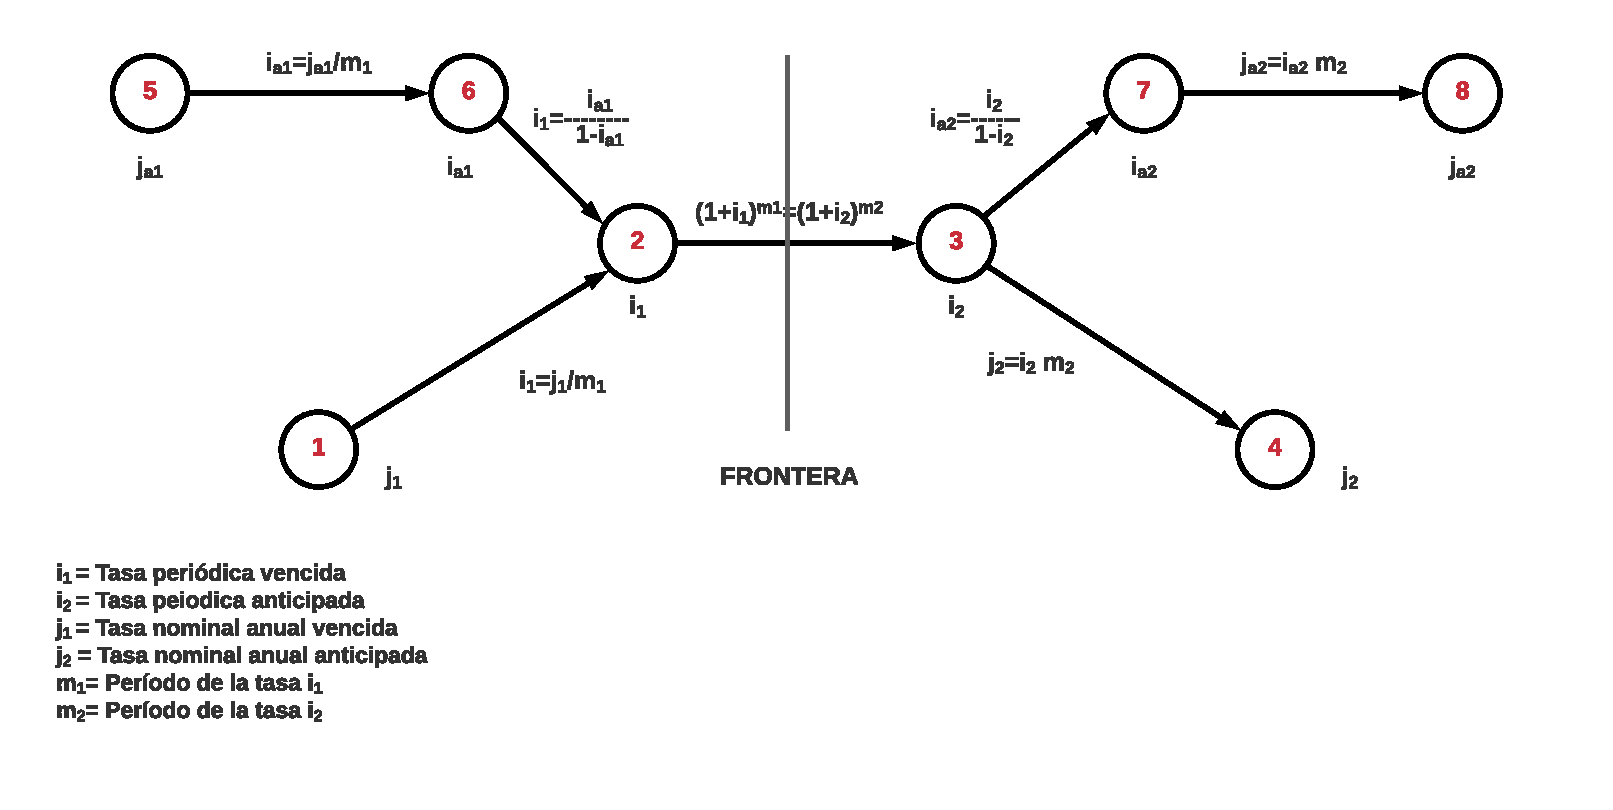
\includegraphics[trim=-5 -5 -5 -5 , scale=0.4]{2_Capitulo/img/ejemplos/6/Capitulo2Ejemplo6.pdf} } \\ \hline

    %%%%%%%%%%%%% FIN INSERCIÓN DE IMAGEN
    %%%%%FIN FLUJO DE CAJA

    %%%%% INICIO DECLARACIÓN FORMULAS
    %%%%%%%%%%% INICIO TITULO
    \rowcolor[HTML]{FFB183}
    \multicolumn{3}{|c|}{\cellcolor[HTML]{FFB183}\textbf{4. Declaración de fórmulas}}                                                                                                  \\ \hline
    %%%%%%%%%%% FIN TITULO
    %%%%%%%%%%% INICIO MATEMÁTICAS

    \multicolumn{2}{|c|}{$(1+i_{1})^{m_{1}} = (1+i_{2})^{m_{2}} \textit{  Equivalencia de tasas}$} & $j_{2}= i_{2}\cdot m_{2}\textit{ 
 Tasa nominal anual}$                                      \\ \hline
    %%%%%%%%%% FIN MATEMÁTICAS
    %%%%%% INICIO DESARROLLO MATEMÁTICO
    \rowcolor[HTML]{FFB183}
    %%%%%%%%%%INICIO TITULO
    \multicolumn{3}{|c|}{\cellcolor[HTML]{FFB183}\textbf{5. Desarrollo matemático}}                                                                                                    \\ \hline
    %%%%%%%%%% FIN TITULO
    %%%%%%%%%% INICIO MATEMÁTICAS
    \multicolumn{2}{|c|}{$(1 + 0,020)^{12}= (1 + i_{2})^{4}$}                                    & $j_{2}=(6,1208\% \textit{ ptd})(4\textit{ ptv}$)                                 \\
    \multicolumn{2}{|c|}{$(1,020)^\frac{12}{4}-1 = i_{2}$}                                      & $j_{2} = 24,4832\% \textit{ natv}$                               \\
    \multicolumn{2}{|c|}{$i_{2}=0,061208 \textit{ ptv} \equiv$  $6,1208\% \textit{ ptv}$}                                      &                                                   \\
    %%%%%%%%%% FIN MATEMÁTICAS
    %%%%%% FIN DESARROLLO MATEMÁTICO
    %%%%%% INICIO RESPUESTA
    \rowcolor[HTML]{FFB183}
    %%%%%%%%%%INICIO TITULO
    \multicolumn{3}{|c|}{\cellcolor[HTML]{FFB183}\textbf{6. Respuesta}}                                                                                                                \\ \hline
    %%%%%%%%%% FIN TITULO
    %%%%%%%%%% INICIO RESPUESTA MATEMÁTICA
    \multicolumn{3}{|c|}{
      \begin{minipage}[t][0.03\textheight][c]{0.8\columnwidth}
        \centering
        ${j_{2} = 24,4832\%  natv}$
      \end{minipage}
    }                                                                                                                                                                                  \\ \hline


    %%%%%%%%%% FIN MATEMÁTICAS
    %%%%%% FIN RESPUESTA
  \end{longtable}
  %Se crean dos lineas en blanco para que no quede el siguiente texto tan pegado
  %\newline \newline %USARLO SI CREES QUE ES NECESARIO
\end{center}

\newpage
%%%%%%%%%%%%%%%%%%% EJERCICIO 7 %%%%%%

\textbf{Ejemplo 7}\\
Suponga que una cuenta de ahorros de un banco le paga una tasa efectiva anual del 24\% nominal anual año vencido.
¿Cuál sería la tasa periódica diaria? Asuma un año de 365 días.\\

%\newpage %USAR SOLO SI EL SOLUCIÓN QUEDA SOLO Y ES NECESARIO BAJARLO A LA SIGUIENTE PAGINA
\textbf{Solución.}\\
%La tabla ira centrada
\begin{center}
  \renewcommand{\arraystretch}{1.5}% Margenes de las celdas
  %Creación de la cuadricula de 3 columnas
  \begin{longtable}[H]{|C{0.3\linewidth}|C{0.3\linewidth}|C{0.3\linewidth}|}
    %Creamos una linea horizontal
    \hline

    %%%%% INICIO ASIGNACIÓN PERíODO FOCAL %%%%%%%
    %%%%%%%%%% INICIO TITULO
    \rowcolor[HTML]{FFB183}
    \multicolumn{3}{|c|}{\cellcolor[HTML]{FFB183}\textbf{1. Asignación período focal}}                                                                                             \\ \hline
    \multicolumn{3}{|c|}{$pf= \textit{No aplica}$}                                                                                                                                 \\ \hline

    %%%%%%%%%% FIN TITULO
    %%%%% INICIO DECLARACIÓN DE VARIABLES %%%%%%%
    %%%%%%%%%% INICIO TITULO
    %Lo que se hace aquí es mezclar las 3 columnas en una sola
    \multicolumn{3}{|c|}{\cellcolor[HTML]{FFB183}\textbf{2. Declaración de variables}}                                                                                             \\ \hline
    %%%%%%%%%% FIN TITULO
    %%%%%%%%%% INICIO DE MATEMÁTICAS
    %Cada & hace referencia al paso de la siguiente columna
    $j_{1}= 24\% \textit{ naav}$                                                                     & $m_{1} = 12 \textit{ pmv}$                     & $i_{2} = ?\% \textit{ pdv} $ \\
    $i_{1}= 2\% \textit{ pmv}$                                                                   &  $m_{2} = 365 \textit{ pdv} $                      &  $j_{2} = ?\% \textit{ nadv} $              \\
         &      
             & \\ \hline

    %%%%%%%%%% FIN DE MATEMÁTICAS
    %%%%% FIN DECLARACIÓN DE VARIABLES


    %%%%% INICIO FLUJO DE CAJA
    \rowcolor[HTML]{FFB183}
    \multicolumn{3}{|c|}{\cellcolor[HTML]{FFB183}\textbf{3. Diagrama de equivalencia de tasas}}                                                                                    \\ \hline
    %Mezclamos 3 columnas y pondremos el dibujo
    %%%%%%%%%%%%% INSERCIÓN DE LA IMAGEN
    %Deberán descargar las imágenes respectivas del drive y pegarlas en la carpeta
    %n_capitulo/img/ejemplos/1/capitulo1ejemplo1.pdf  (el /1/ es el numero del ejemplo)

    \multicolumn{3}{|c|}{ 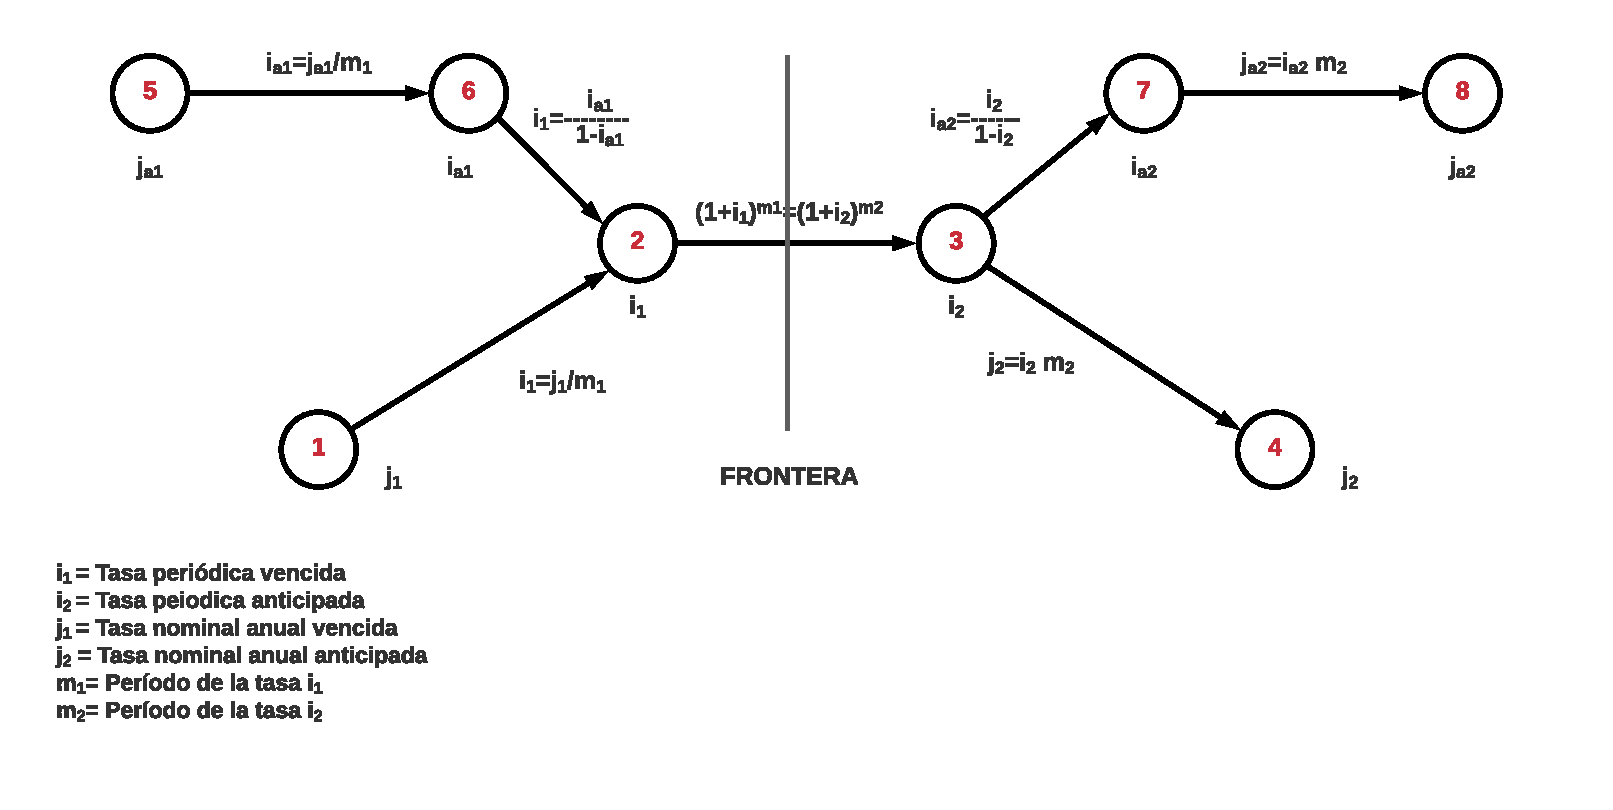
\includegraphics[trim=-5 -5 -5 -5 , scale=0.4]{2_Capitulo/img/ejemplos/6/Capitulo2Ejemplo6.pdf} } \\ \hline
    
    %%%%%%%%%%%%% FIN INSERCIÓN DE IMAGEN
    %%%%%FIN FLUJO DE CAJA

    %%%%% INICIO DECLARACIÓN FORMULAS
    %%%%%%%%%%% INICIO TITULO
    \rowcolor[HTML]{FFB183}
    \multicolumn{3}{|c|}{\cellcolor[HTML]{FFB183}\textbf{4. Declaración de fórmulas}}                                                                                              \\ \hline
    %%%%%%%%%%% FIN TITULO
    %%%%%%%%%%% INICIO MATEMÁTICAS

    \multicolumn{2}{|c|}{$(1+i_{1})^{m_{1}} = (1+i_{2})^{m_{2}} \textit{ Equivalencia de tasas}$} & $j_{2}= i_{2} \cdot m_{2}\textit{ Tasa nominal anual}$                                \\ \hline
    %%%%%%%%%% FIN MATEMÁTICAS
    %%%%%% INICIO DESARROLLO MATEMÁTICO
    \rowcolor[HTML]{FFB183}
    %%%%%%%%%%INICIO TITULO
    \multicolumn{3}{|c|}{\cellcolor[HTML]{FFB183}\textbf{5. Desarrollo matemático}}                                                                                                \\ \hline
    %%%%%%%%%% FIN TITULO
    %%%%%%%%%% INICIO MATEMÁTICAS
    \multicolumn{2}{|c|}{$(1 + 0,02)^{12}= (1 + i_{2})^{365}$}                                    & $j_{2}=(0,065\% \textit{ pdv}) (365\textit{ pdv}) $                                               \\
    \multicolumn{2}{|c|}{$(1,26824)^\frac{1}{365}-1 = i_{2}$}                                     &  $j_{2} = 23,771\% \textit{ nadv}$                                                                               \\
    \multicolumn{2}{|c|}{$i_{2}=0.065\% \textit{ pdv}$}                                           &                                                                                                                \\

    %%%%%%%%%% FIN MATEMÁTICAS
    %%%%%% FIN DESARROLLO MATEMÁTICO
    %%%%%% INICIO RESPUESTA
    \rowcolor[HTML]{FFB183}
    %%%%%%%%%%INICIO TITULO
    \multicolumn{3}{|c|}{\cellcolor[HTML]{FFB183}\textbf{6. Respuesta}}                                                                                                            \\ \hline
    %%%%%%%%%% FIN TITULO
    %%%%%%%%%% INICIO RESPUESTA MATEMÁTICA
    \multicolumn{3}{|c|}{
      \begin{minipage}[t][0.03\textheight][c]{0.8\columnwidth}
        \centering
        ${j_{2} = 23,771\% nadv}$
      \end{minipage}
    }                                                                                                                                                                              \\ \hline


    %%%%%%%%%% FIN MATEMÁTICAS
    %%%%%% FIN RESPUESTA
  \end{longtable}
  %Se crean dos lineas en blanco para que no quede el siguiente texto tan pegado
  %\newline \newline %USARLO SI CREES QUE ES NECESARIO
\end{center}
%%%%%%%%%%%%%%%%%%%%%%%%%%FIN EJERCICIO 7 %%%%%%%%%%%%%%%%%%%%%%%%%%%
%%%%%%%% EJERCICIO 8 %%%%%%
    %%%% revisar :) %%%%

    \textbf{Ejemplo 8}\\
    ¿Cuál es la tasa de interés nominal anual trimestre vencido, equivalente al 24\% nominal anual mes vencido? \\ \\
    %\newpage %USAR SOLO SI EL SOLUCIÓN QUEDA SOLO Y ES NECESARIO BAJARLO A LA SIGUIENTE PAGINA
    \textbf{Solución.}\\
    %La tabla ira centrada
    \begin{center}
      \renewcommand{\arraystretch}{1.5}% Margenes de las celdas
      %Creación de la cuadricula de 3 columnas
      \begin{longtable}[H]{|C{0.3\linewidth}|C{0.3\linewidth}|C{0.3\linewidth}|}
        %Creamos una linea horizontal
        \hline
        %Definimos el color de la primera fila
        \rowcolor[HTML]{FFB183}
        %%%%% INICIO ASIGNACIÓN PERíODO FOCAL %%%%%%%
        %%%%%%%%%% INICIO TITULO
        %Lo que se hace aquí es mezclar las 3 columnas en una sola
        \multicolumn{3}{|c|}{\cellcolor[HTML]{FFB183}\textbf{1. Asignación período focal}}                                                                   \\ \hline
        \multicolumn{3}{|c|}{$pf= \textit{No aplica}$}                                                                                                       \\ \hline
        %%%%%%%%%% FIN TITULO
    
        %%%%% INICIO DECLARACIÓN DE VARIABLES %%%%%%%
        %%%%%%%%%% INICIO TITULO
        %Lo que se hace aquí es mezclar las 3 columnas en una sola
        \multicolumn{3}{|c|}{\cellcolor[HTML]{FFB183}\textbf{2. Declaración de variables}}                                                                                             \\ \hline
        %%%%%%%%%% FIN TITULO
        %%%%%%%%%% INICIO DE MATEMÁTICAS
        %Cada & hace referencia al paso de la siguiente columna
        $j_{1}= 24\% \textit{ namv}$                                                                     & $m_{1} = 12 \textit{ pmv}$                     & $i_{2} = ?\% \textit{ ptv} $ \\
        $i_{1}= 2\% \textit{ pmv}$                                                                   &  $m_{2} = 4 \textit{ ptv} $                      &  $j_{2} = ?\% \textit{ natv} $  \\
             &       
              &  \\ \hline
    
        %%%%%%%%%% FIN DE MATEMÁTICAS
        %%%%% FIN DECLARACIÓN DE VARIABLES
    
    
        %%%%% INICIO FLUJO DE CAJA
        \rowcolor[HTML]{FFB183}
        \multicolumn{3}{|c|}{\cellcolor[HTML]{FFB183}\textbf{3. Diagrama equivalencia de tasas}}                                                             \\ \hline
        %Mezclamos 3 columnas y pondremos el dibujo
        %%%%%%%%%%%%% INSERCIÓN DE LA IMAGEN
        %Deberán descargar las imágenes respectivas del drive y pegarlas en la carpeta
        %n_capitulo/img/ejemplos/1/capitulo1ejemplo1.pdf  (el /1/ es el numero del ejemplo)
    
        \multicolumn{3}{|c|}{ 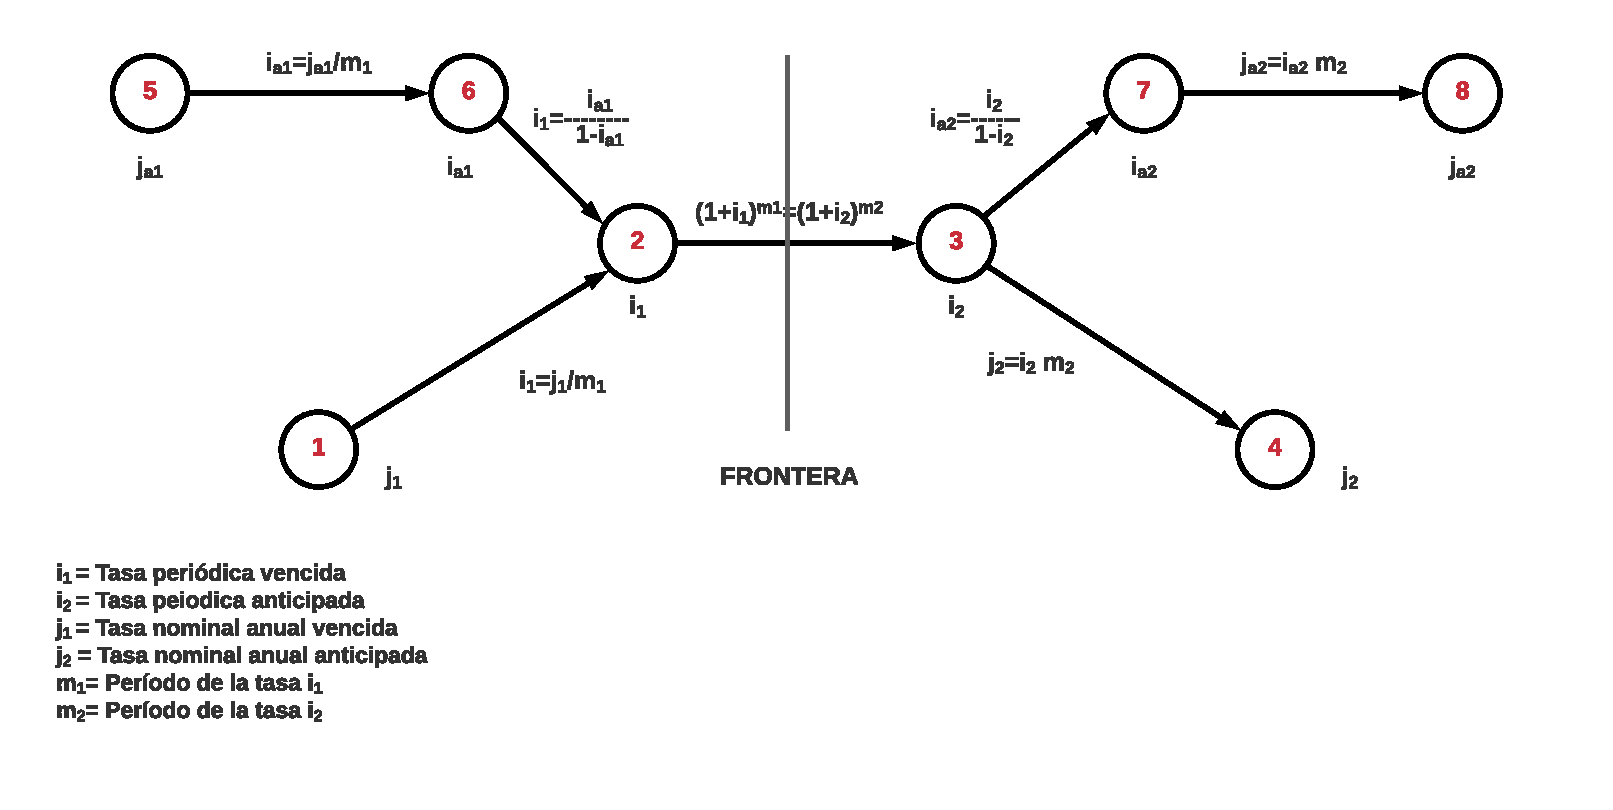
\includegraphics[trim=-5 -5 -5 -5 , scale=0.4]{2_Capitulo/img/ejemplos/6/Capitulo2Ejemplo6.pdf} } \\ \hline
        
        %%%%%%%%%%%%% FIN INSERCIÓN DE IMAGEN
        %%%%%FIN FLUJO DE CAJA
    
        %%%%% INICIO DECLARACIÓN FORMULAS
        %%%%%%%%%%% INICIO TITULO
        \rowcolor[HTML]{FFB183}
        \multicolumn{3}{|c|}{\cellcolor[HTML]{FFB183}\textbf{4. Declaración de fórmulas}}                                                                    \\ \hline
        %%%%%%%%%%% FIN TITULO
        %%%%%%%%%%% INICIO MATEMÁTICAS
    
        \multicolumn{2}{|c|}{$(1 + i_{1})^{m_{1}}= (1 + i_{2})^{m_{2}} \textit{ Equivalencia de tasas}$} & {$j_{2}=i_{2}\cdot m_{2} \textit{ Tasa nominal anual}$} \\ \hline
        %%%%%%%%%% FIN MATEMÁTICAS
        %%%%%% INICIO DESARROLLO MATEMÁTICO
        \rowcolor[HTML]{FFB183}
        %%%%%%%%%%INICIO TITULO
        \multicolumn{3}{|c|}{\cellcolor[HTML]{FFB183}\textbf{5. Desarrollo matemático}}                                                                      \\ \hline
        %%%%%%%%%% FIN TITULO
        %%%%%%%%%% INICIO MATEMÁTICAS
        \multicolumn{2}{|c|}{$(1 + 0,02)^{12}= (1 + i_{2})^{4} $}                                     & $j_{2}=(6,121\% \textit{ ptv}) (4 \textit{ ptv})$              \\
        \multicolumn{2}{|c|}{$(1,02)^{\frac{12}{4}}-1=i_{2}$ }                                          & $j_{2} = 24,48\% \textit{ natv}$                                                  \\
        \multicolumn{2}{|c|}{$i_{2}=0,061208 \textit{ ptv} \equiv$ $6,121\% \textit{ ptv}$}                                            &                                                                             \\ \hline
    
        %%%%%%%%%% FIN MATEMÁTICAS
        %%%%%% FIN DESARROLLO MATEMÁTICO
        %%%%%% INICIO RESPUESTA
        \rowcolor[HTML]{FFB183}
        %%%%%%%%%%INICIO TITULO
        \multicolumn{3}{|c|}{\cellcolor[HTML]{FFB183}\textbf{6. Respuesta}}                                                                                  \\ \hline
        %%%%%%%%%% FIN TITULO
        %%%%%%%%%% INICIO RESPUESTA MATEMÁTICA
        \multicolumn{3}{|c|}{
    
          \begin{minipage}[t][0.07\textheight][c]{0.8\columnwidth}
            \centering
            ${j_{2} = 24,48\%  natv}$
          \end{minipage}
        }                                                                                                                                                    \\ \hline
    
        %%%%%%%%%% FIN MATEMÁTICAS
        %%%%%% FIN RESPUESTA
      \end{longtable}
      %Se crean dos lineas en blanco para que no quede el siguiente texto tan pegado
      %\newline \newline %USARLO SI CREES QUE ES NECESARIO
    \end{center}
    %%%%%%%%%%%%%%%%%%%%%%%%%%FIN EJERCICIO 8 %%%%%%%%%%%%%%%%%%%%%%%%%%%
    
%%%%%%%%%%%%%%%%%%% EJERCICIO 9  %%%%%%

\textbf{Ejemplo 9}\\
Dado el 24\% nominal anual mes vencido hallar:\\

%%%%%%%%%%%%%%%%%%% EJERCICIO 9.a  %%%%%%
\textbf{Parte a.} Una tasa efectiva nominal anual año vencido. \\
%\newpage %USAR SOLO SI EL SOLUCIÓN QUEDA SOLO Y ES NECESARIO BAJARLO A LA SIGUIENTE PAGINA
\textbf{Solución a.}\\
%La tabla ira centrada
\begin{center}
  \renewcommand{\arraystretch}{1.5}% Margenes de las celdas
  %Creación de la cuadricula de 3 columnas
  \begin{longtable}[H]{|C{0.3\linewidth}|C{0.3\linewidth}|C{0.3\linewidth}|}
    %Creamos una linea horizontal
    \hline
    %Definimos el color de la primera fila
    \rowcolor[HTML]{FFB183}
    %%%%% INICIO ASIGNACIÓN PERíODO FOCAL %%%%%%%
    %%%%%%%%%% INICIO TITULO
    %Lo que se hace aquí es mezclar las 3 columnas en una sola
    \multicolumn{3}{|c|}{\cellcolor[HTML]{FFB183}\textbf{1. Asignación período focal}}                                                                                                  \\ \hline
    \multicolumn{3}{|c|}{$pf= \textit{No aplica}$}                                                                                                                                      \\ \hline
    %%%%%%%%%% FIN TITULO
    %%%%% INICIO DECLARACIÓN DE VARIABLES %%%%%%%
    %%%%%%%%%% INICIO TITULO
    %Lo que se hace aquí es mezclar las 3 columnas en una sola
    \multicolumn{3}{|c|}{\cellcolor[HTML]{FFB183}\textbf{2. Declaración de variables}}                                                                                                  \\ \hline
    %%%%%%%%%% FIN TITULO
    %%%%%%%%%% INICIO DE MATEMÁTICAS
    %Cada & hace referencia al paso de la siguiente columna
    $j_{1} = 24\% \textit{ namv}$                                                               & $m_{1} = 12  \textit{ pmv}  $                            & $i_{2} = ?\% \textit{ pmv} $ \\
    $i_{1}= \frac{24\% \textit{ namv}}{12 \textit{ pmv}} = 2\% \textit{ pmv}$             & $m_{2} = 1 \textit{ pav} $                                     & $j_{2} = ?\% \textit{ naav} $                              \\                                                              &                                                       &                               \\ \hline

    %%%%%%%%%% FIN DE MATEMÁTICAS
    %%%%% FIN DECLARACIÓN DE VARIABLES

    %%%%% INICIO FLUJO DE CAJA
    \rowcolor[HTML]{FFB183}
    \multicolumn{3}{|c|}{\cellcolor[HTML]{FFB183}\textbf{3. Diagrama de equivalencia de tasas}}                                                                                         \\ \hline
    %Mezclamos 3 columnas y pondremos el dibujo
    %%%%%%%%%%%%% INSERCIÓN DE LA IMAGEN
    %Deberán descargar las imágenes respectivas del drive y pegarlas en la carpeta
    %n_capitulo/img/ejemplos/1/capitulo1ejemplo1.pdf  (el /1/ es el numero del ejemplo)

    \multicolumn{3}{|c|}{ 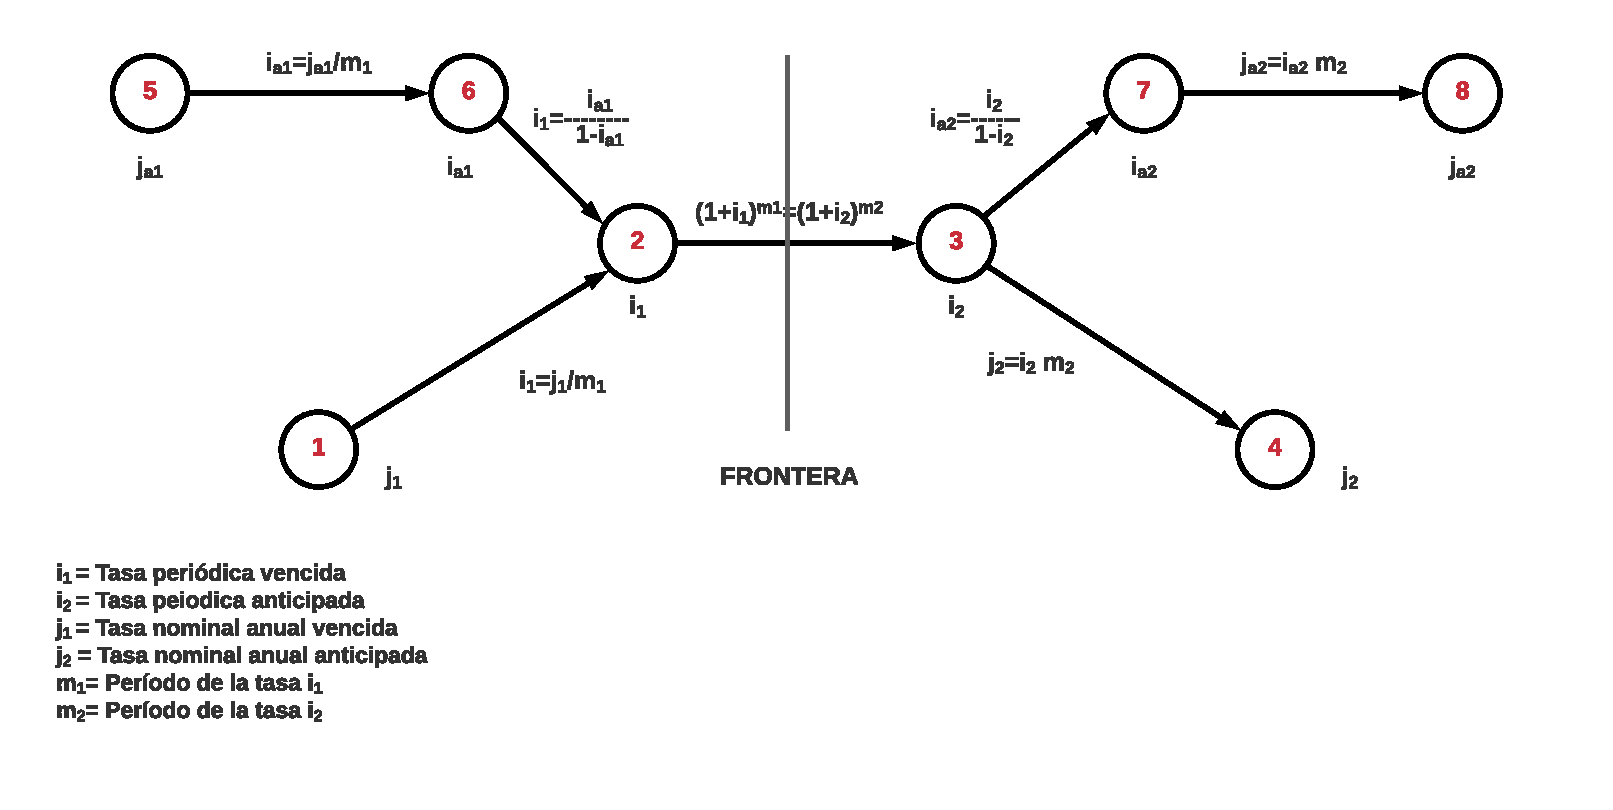
\includegraphics[trim=-5 -5 -5 -5 , scale=0.4]{2_Capitulo/img/ejemplos/6/Capitulo2Ejemplo6.pdf} } \\ \hline
    
    %%%%%%%%%%%%% FIN INSERCIÓN DE IMAGEN
    %%%%%FIN FLUJO DE CAJA

    %%%%% INICIO DECLARACIÓN FORMULAS
    %%%%%%%%%%% INICIO TITULO
    \rowcolor[HTML]{FFB183}
    \multicolumn{3}{|c|}{\cellcolor[HTML]{FFB183}\textbf{4. Declaración de fórmulas}}                                                                                                   \\ \hline
    %%%%%%%%%%% FIN TITULO
    %%%%%%%%%%% INICIO MATEMÁTICAS

    \multicolumn{2}{|c|}{$(1+i_{1})^{m_{1}}=(1+i_{2})^{m_{2}} \textit{ Equivalencia de tasas}$} & $j_{2}=i_{2}\cdot m_{2} \textit{ Tasa nominal anual}$                                 \\ \hline
    %%%%%%%%%% FIN MATEMÁTICAS
    %%%%%% INICIO DESARROLLO MATEMÁTICO
    \rowcolor[HTML]{FFB183}
    %%%%%%%%%%INICIO TITULO
    \multicolumn{3}{|c|}{\cellcolor[HTML]{FFB183}\textbf{5. Desarrollo matemático}}                                                                                                     \\ \hline
    %%%%%%%%%% FIN TITULO
    %%%%%%%%%% INICIO MATEMÁTICAS
    \multicolumn{2}{|c|}{$(1 + 0,02)^{12}= (1 + i_{2})^{1} $}                                 & {$j_{2}=(26,824\% \textit{ pav})( 1\textit{ pav})$}                                                     \\
    \multicolumn{2}{|c|}{$(1,02)^{\frac{12}{1}}-1=i_{2}$ }                                      & {$j_{2} = 26,824\% \textit{ naav}$}                                                                                      \\
    \multicolumn{2}{|c|}{$i_{2}= 0,26824 \textit{ ptv} \equiv 26,824\% \textit{ pav}$}                                   &                                                                                                                                         \\ \hline

    %%%%%%%%%% FIN MATEMÁTICAS
    %%%%%% FIN DESARROLLO MATEMÁTICO
    %%%%%% INICIO RESPUESTA
    \rowcolor[HTML]{FFB183}
    %%%%%%%%%%INICIO TITULO
    \multicolumn{3}{|c|}{\cellcolor[HTML]{FFB183}\textbf{6. Respuesta}}                                                                                                                 \\ \hline
    %%%%%%%%%% FIN TITULO
    %%%%%%%%%% INICIO RESPUESTA MATEMÁTICA
    \multicolumn{3}{|c|}{
      \begin{minipage}[t][0.03\textheight][c]{0.8\columnwidth}
        \centering
        ${j_{2} = 26,824\%   naav}$
      \end{minipage}
    }                                                                                                                                                                                   \\ \hline
    %%%%%%%%%% FIN MATEMÁTICAS
    %%%%%% FIN RESPUESTA
  \end{longtable}
  %Se crean dos lineas en blanco para que no quede el siguiente texto tan pegado
  %\newline \newline %USARLO SI CREES QUE ES NECESARIO
\end{center}
%%%%%%%%%%%%%%%%%%% FIN EJERCICIO 9.a  %%%%%%%%%%%%%%%%%%%%%%%%%%%%%%
\newpage
%%%%%%%%%%%%%%%%%%% EJERCICIO 9.b  %%%%%%
\textbf{Parte b.} Una tasa nominal anual semestre vencido. \\
%\newpage %USAR SOLO SI EL SOLUCIÓN QUEDA SOLO Y ES NECESARIO BAJARLO A LA SIGUIENTE PAGINA
\textbf{Solución b.}\\
%La tabla ira centrada
\begin{center}
   \renewcommand{\arraystretch}{1.5}% Margenes de las celdas
   %Creación de la cuadricula de 3 columnas
   \begin{longtable}[H]{|C{0.3\linewidth}|C{0.3\linewidth}|C{0.3\linewidth}|}
      %Creamos una linea horizontal
      \hline
      %Definimos el color de la primera fila
      \rowcolor[HTML]{FFB183}
      %%%%% INICIO ASIGNACIÓN PERíODO FOCAL %%%%%%%
      %%%%%%%%%% INICIO TITULO
      %Lo que se hace aquí es mezclar las 3 columnas en una sola
      \multicolumn{3}{|c|}{\cellcolor[HTML]{FFB183}\textbf{1. Asignación período focal}}                                                                                                  \\ \hline
      \multicolumn{3}{|c|}{$pf= \textit{No aplica}$}                                                                                                                                      
      \\ \hline
      %%%%%%%%%% FIN TITULO
      %%%%% INICIO DECLARACIÓN DE VARIABLES %%%%%%%
      %%%%%%%%%% INICIO TITULO
      %Lo que se hace aquí es mezclar las 3 columnas en una sola
      \multicolumn{3}{|c|}{\cellcolor[HTML]{FFB183}\textbf{2. Declaración de variables}}                                                                                                  \\ \hline
      %%%%%%%%%% FIN TITULO
      %%%%%%%%%% INICIO DE MATEMÁTICAS
      %Cada & hace referencia al paso de la siguiente columna
      $j_{1} = 24\% \textit{ namv}$          & $m_{1} = 12  \textit{ pmv}$                            & $i_{2} = ?\% \textit{ psv} $ \\
      $i_{1}= 2\% \textit{ pmv}$       & $m_{2} = 2 \textit{ psv} $                                                      &   $j_{2} = ?\% \textit{ nasv} $                             \\                                                            &                                                       &                               \\ \hline

      %%%%%%%%%% FIN DE MATEMÁTICAS
      %%%%% FIN DECLARACIÓN DE VARIABLES

      %%%%% INICIO FLUJO DE CAJA
      \rowcolor[HTML]{FFB183}
      \multicolumn{3}{|c|}{\cellcolor[HTML]{FFB183}\textbf{3. Diagrama de equivalencia de tasas}}                                                                                         \\ \hline
      %Mezclamos 3 columnas y pondremos el dibujo
      %%%%%%%%%%%%% INSERCIÓN DE LA IMAGEN
      %Deberán descargar las imágenes respectivas del drive y pegarlas en la carpeta
      %n_capitulo/img/ejemplos/1/capitulo1ejemplo1.pdf  (el /1/ es el numero del ejemplo)

      \multicolumn{3}{|c|}{ 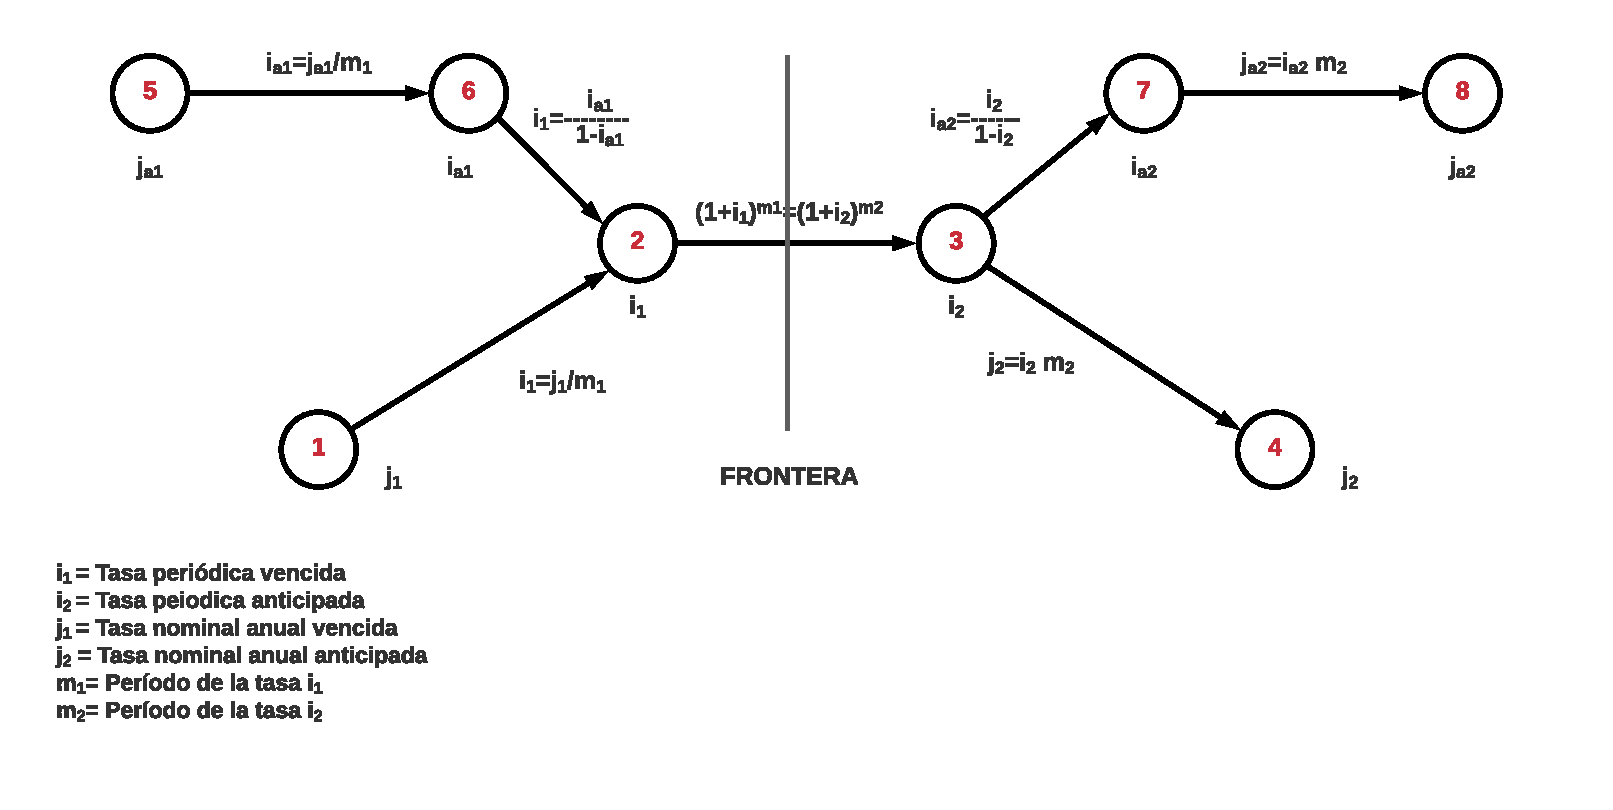
\includegraphics[trim=-5 -5 -5 -5 , scale=0.4]{2_Capitulo/img/ejemplos/6/Capitulo2Ejemplo6.pdf} } \\ \hline
      
      %%%%%%%%%%%%% FIN INSERCIÓN DE IMAGEN
      %%%%%FIN FLUJO DE CAJA

      %%%%% INICIO DECLARACIÓN FORMULAS
      %%%%%%%%%%% INICIO TITULO
      \rowcolor[HTML]{FFB183}
      \multicolumn{3}{|c|}{\cellcolor[HTML]{FFB183}\textbf{4. Declaración de fórmulas}}                                                                                                   \\ \hline
      %%%%%%%%%%% FIN TITULO
      %%%%%%%%%%% INICIO MATEMÁTICAS

      \multicolumn{2}{|c|}{$(1+i_{1})^{m_{1}}=(1+i_{2})^{m_{2}} \textit{ Equivalencia de tasas}$} & $j_{2}=i_{2}\cdot m_{2} \textit{ Tasa nominal anual}$                                 \\ \hline
      %%%%%%%%%% FIN MATEMÁTICAS
      %%%%%% INICIO DESARROLLO MATEMÁTICO
      \rowcolor[HTML]{FFB183}
      %%%%%%%%%%INICIO TITULO
      \multicolumn{3}{|c|}{\cellcolor[HTML]{FFB183}\textbf{5. Desarrollo matemático}}                                                                                                     \\ \hline
      %%%%%%%%%% FIN TITULO
      %%%%%%%%%% INICIO MATEMÁTICAS
      \multicolumn{2}{|c|}{$(1 + 0,02\%)^{12}= (1 + i_{2})^{2} $}                                 & {$j_{2}=(12,616\% \textit{ psv})(2\textit{ psv})$}                                                   \\
      \multicolumn{2}{|c|}{$(1,02)^{6}-1=i_{2}$ }                                      &  {$j_{2} = 25,232\% \textit{ nasv}$}                                                                                        \\
      \multicolumn{2}{|c|}{$i_{2}= 0,12616 \textit{ psv} \equiv 12,616\% \textit{ psv}$}                                  &                                                                                                                                                                \\ \hline
      %%%%%%%%%% FIN MATEMÁTICAS
      %%%%%% FIN DESARROLLO MATEMÁTICO
      %%%%%% INICIO RESPUESTA
      \rowcolor[HTML]{FFB183}
      %%%%%%%%%%INICIO TITULO
      \multicolumn{3}{|c|}{\cellcolor[HTML]{FFB183}\textbf{6. Respuesta}}                                                                                                                 \\ \hline
      %%%%%%%%%% FIN TITULO
      %%%%%%%%%% INICIO RESPUESTA MATEMÁTICA
      \multicolumn{3}{|c|}{

         \begin{minipage}[t][0.03\textheight][c]{0.8\columnwidth}
            \centering
            ${j_{2} = 25,232\%  nasv}$
         \end{minipage}
      }                                                                                                                                                                                   \\ \hline


      %%%%%%%%%% FIN MATEMÁTICAS
      %%%%%% FIN RESPUESTA
   \end{longtable}
   %Se crean dos lineas en blanco para que no quede el siguiente texto tan pegado
   %\newline \newline %USARLO SI CREES QUE ES NECESARIO
\end{center}
%%%%%%%%%%%%%%%%%%% FIN EJERCICIO 9.b  %%%%%%%%%%%%%%%%%%%%%%%%%%%%%%
\newpage
%%%%%%%%%%%%%%%%%%% EJERCICIO 9.c  %%%%%%
\textbf{Parte c.} Una tasa periódica bimensual vencida. \\
%\newpage %USAR SOLO SI EL SOLUCIÓN QUEDA SOLO Y ES NECESARIO BAJARLO A LA SIGUIENTE PAGINA
\textbf{Solución c.}\\
%La tabla ira centrada
\begin{center}
   \renewcommand{\arraystretch}{1.5}% Margenes de las celdas
   %Creación de la cuadricula de 3 columnas
   \begin{longtable}[H]{|C{0.3\linewidth}|C{0.3\linewidth}|C{0.3\linewidth}|}
      %Creamos una linea horizontal
      \hline
      %Definimos el color de la primera fila
      \rowcolor[HTML]{FFB183}
      %%%%% INICIO ASIGNACIÓN PERíODO FOCAL %%%%%%%
      %%%%%%%%%% INICIO TITULO
      %Lo que se hace aquí es mezclar las 3 columnas en una sola
      \multicolumn{3}{|c|}{\cellcolor[HTML]{FFB183}\textbf{1. Asignación período focal}}                                                                                                 \\ \hline
      \multicolumn{3}{|c|}{$pf= \textit{No aplica}$}                                                                                                                                    
      \\ \hline
      %%%%%%%%%% FIN TITULO
      %%%%% INICIO DECLARACIÓN DE VARIABLES %%%%%%%
      %%%%%%%%%% INICIO TITULO
      %Lo que se hace aquí es mezclar las 3 columnas en una sola
      \multicolumn{3}{|c|}{\cellcolor[HTML]{FFB183}\textbf{2. Declaración de variables}}                                                                                                 \\ \hline
      %%%%%%%%%% FIN TITULO
      %%%%%%%%%% INICIO DE MATEMÁTICAS
      %Cada & hace referencia al paso de la siguiente columna

      $j_{1} = 24\% \textit{ namv}$          & $m_{1} = 12  \textit{ pmv}$                            & $i_{2} = ?\% \textit{ pbv} $ \\
      $i_{1}= 2\% \textit{ pmv}$       & $m_{2} = 2 \textit{ pbv} $                                                      &   $j_{2} = ?\% \textit{ nasv} $                             \\                                                            &                                                       &                               \\ \hline




      
      %%%%%%%%%% FIN DE MATEMÁTICAS
      %%%%% FIN DECLARACIÓN DE VARIABLES

      %%%%% INICIO FLUJO DE CAJA
      \rowcolor[HTML]{FFB183}
      \multicolumn{3}{|c|}{\cellcolor[HTML]{FFB183}\textbf{3. Diagrama de equivalencia de tasas}}                                                                                        \\ \hline
      %Mezclamos 3 columnas y pondremos el dibujo
      %%%%%%%%%%%%% INSERCIÓN DE LA IMAGEN
      %Deberán descargar las imágenes respectivas del drive y pegarlas en la carpeta
      %n_capitulo/img/ejemplos/1/capitulo1ejemplo1.pdf  (el /1/ es el numero del ejemplo)

      \multicolumn{3}{|c|}{ 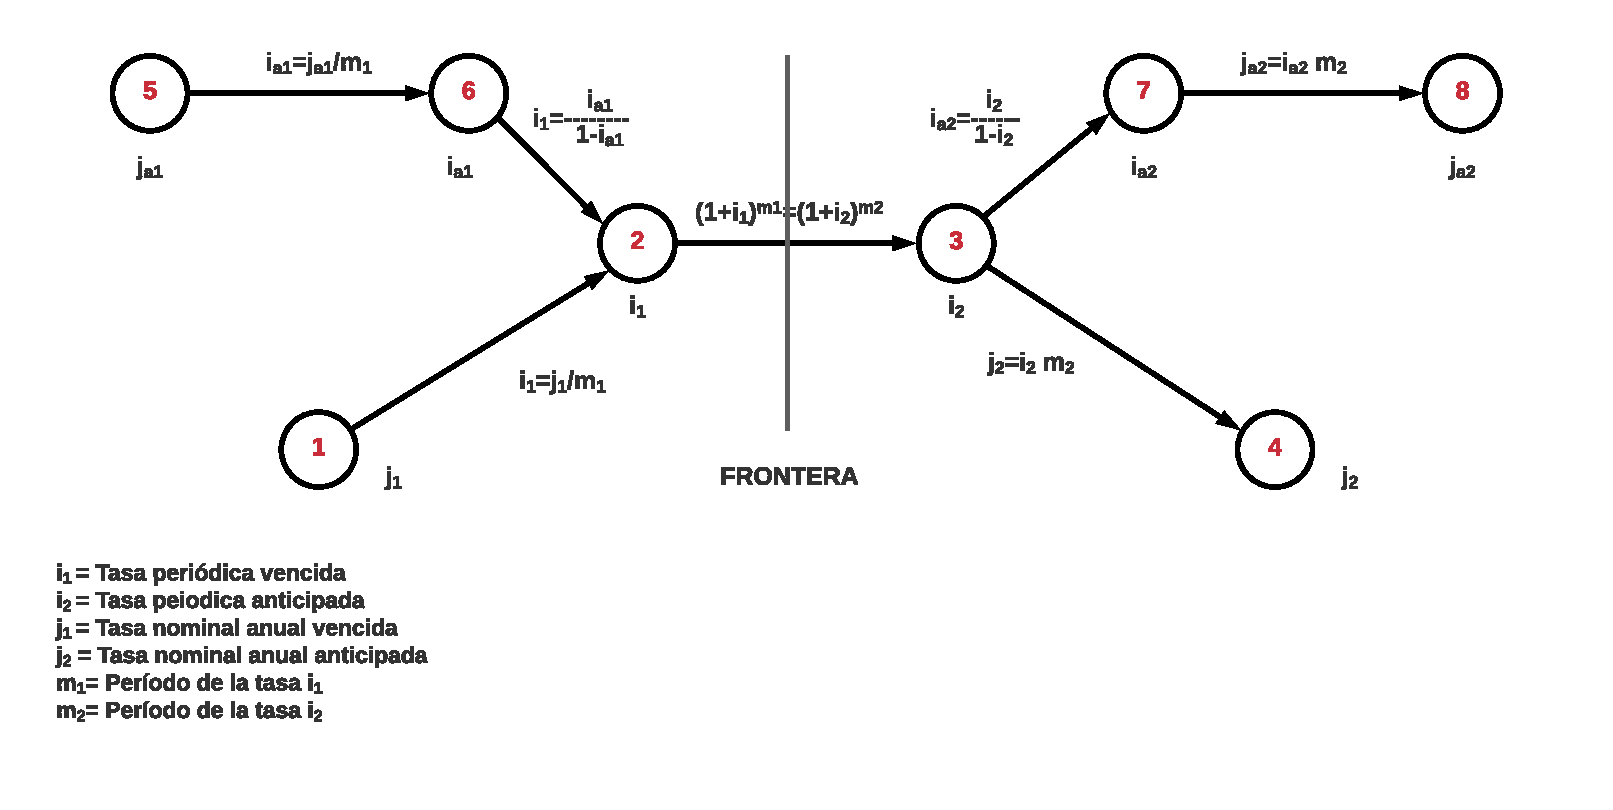
\includegraphics[trim=-5 -5 -5 -5 , scale=0.4]
      {2_Capitulo/img/ejemplos/6/Capitulo2Ejemplo6.pdf} } 
       \\ \hline
      
      %%%%%%%%%%%%% FIN INSERCIÓN DE IMAGEN
      %%%%%FIN FLUJO DE CAJA

      %%%%% INICIO DECLARACIÓN FORMULAS
      %%%%%%%%%%% INICIO TITULO
      \rowcolor[HTML]{FFB183}
      \multicolumn{3}{|c|}{\cellcolor[HTML]{FFB183}\textbf{4. Declaración de fórmulas}}                                                                                                  \\ \hline
      %%%%%%%%%%% FIN TITULO
      %%%%%%%%%%% INICIO MATEMÁTICAS

      \multicolumn{2}{|c|}{$(1+i_{1})^{m_{1}}=(1+i_{2})^{m_{2}} \textit{ Equivalencia de tasas}$} & $j_{2}=i_{2}\cdot m_{2} \textit{ Tasa nominal anual}$                                \\ \hline
      %%%%%%%%%% FIN MATEMÁTICAS
      %%%%%% INICIO DESARROLLO MATEMÁTICO
      \rowcolor[HTML]{FFB183}
      %%%%%%%%%%INICIO TITULO
      \multicolumn{3}{|c|}{\cellcolor[HTML]{FFB183}\textbf{5. Desarrollo matemático}}                                                                                                    \\ \hline
      %%%%%%%%%% FIN TITULO
      %%%%%%%%%% INICIO MATEMÁTICAS
      \multicolumn{2}{|c|}{$(1 + 0,02\%)^{12}= (1 + i_{2})^{6} $}                                 & {$j_{2}=(4,04\% \textit{ pbv})(6\textit{ pbv})$}                                                    \\
      \multicolumn{2}{|c|}{$(1,02)^{2}-1=i_{2}$ }                                      & {$j_{2} = 24,24\% \textit{ nabv}$}                                                                                        \\
      \multicolumn{2}{|c|}{$i_{2}= 0,0404 \textit{ pbv} \equiv 4,04\% \textit{ pbv}$}                                          &                                                                                                              \\ \hline
      %%%%%%%%%% FIN MATEMÁTICAS
      %%%%%% FIN DESARROLLO MATEMÁTICO
      %%%%%% INICIO RESPUESTA
      \rowcolor[HTML]{FFB183}
      %%%%%%%%%%INICIO TITULO
      \multicolumn{3}{|c|}{\cellcolor[HTML]{FFB183}\textbf{6. Respuesta}}                                                                                                                \\ \hline
      %%%%%%%%%% FIN TITULO
      %%%%%%%%%% INICIO RESPUESTA MATEMÁTICA
      \multicolumn{3}{|c|}{
         \begin{minipage}[t][0.03\textheight][c]{0.8\columnwidth}
            \centering
            ${j_{2} = 24,24\% nabv}$
            
         \end{minipage}
      }     

                                             \\ \hline
      %%%%%%%%%% FIN MATEMÁTICAS
      %%%%%% FIN RESPUESTA
   \end{longtable}
   %Se crean dos lineas en blanco para que no quede el siguiente texto tan pegado
   %\newline \newline %USARLO SI CREES QUE ES NECESARIO
\end{center}
%%%%%%%%%%%%%%%%%%% FIN EJERCICIO 9.c  %%%%%%%%%%%%%%%%%%%%%%%%%%%%%%
\newpage
%%%%%%%%%%%%%%%%%%% EJERCICIO 9.d  %%%%%%
\textbf{Parte d.} Una tasa nominal anual semestre anticipado. \\
%\newpage %USAR SOLO SI EL SOLUCIÓN QUEDA SOLO Y ES NECESARIO BAJARLO A LA SIGUIENTE PAGINA
\textbf{Solución d.}\\
%La tabla ira centrada
\begin{center}
   \renewcommand{\arraystretch}{1.5}% Margenes de las celdas
   %Creación de la cuadricula de 3 columnas
   \begin{longtable}[H]{|c|c|c|}
      %Creamos una linea horizontal
      \hline
      %Definimos el color de la primera fila
      \rowcolor[HTML]{FFB183}
      %%%%% INICIO ASIGNACIÓN PERíODO FOCAL %%%%%%%
      %%%%%%%%%% INICIO TITULO
      %Lo que se hace aquí es mezclar las 3 columnas en una sola
      \multicolumn{3}{|c|}{\cellcolor[HTML]{FFB183}\textbf{1. Asignación período focal}}                                                                                                                   \\ \hline
      \multicolumn{3}{|c|}{$pf= \textit{No aplica}$}                                                                                                                                              
      \\ \hline
      %%%%%%%%%% FIN TITULO
      %%%%% INICIO DECLARACIÓN DE VARIABLES %%%%%%%
      %%%%%%%%%% INICIO TITULO
      %Lo que se hace aquí es mezclar las 3 columnas en una sola
      \multicolumn{3}{|c|}{\cellcolor[HTML]{FFB183}\textbf{2. Declaración de variables}}                                                                                                                       \\ \hline
      %%%%%%%%%% FIN TITULO
      %%%%%%%%%% INICIO DE MATEMÁTICAS
      %Cada & hace referencia al paso de la siguiente columna
      $j_{1} = 24\% \textit{ namv}$ & $m_{1} = 12  \textit{ pmv}  $  & $i_{2} = ?\% \textit{ psv} $ \\ 
      $i_{1} = 2\% \textit{ pmv}$ & $m_{2} = 2 \textit{ psa} $     &  $i_{a2} = ?\% \textit{ psa} $  \\
       &         & $j_{a2} = ?\% \textit{ nasa} $                \\ \hline
      %%%%%%%%%% FIN DE MATEMÁTICAS
      %%%%% FIN DECLARACIÓN DE VARIABLES

      %%%%% INICIO FLUJO DE CAJA
      \rowcolor[HTML]{FFB183}
      \multicolumn{3}{|c|}{\cellcolor[HTML]{FFB183}\textbf{3. Diagrama de equivalencia de tasas}}                                                                                                              \\ \hline
      %Mezclamos 3 columnas y pondremos el dibujo
      %%%%%%%%%%%%% INSERCIÓN DE LA IMAGEN
      %Deberán descargar las imágenes respectivas del drive y pegarlas en la carpeta
      %n_capitulo/img/ejemplos/1/capitulo1ejemplo1.pdf  (el /1/ es el numero del ejemplo)

      \multicolumn{3}{|c|}{ 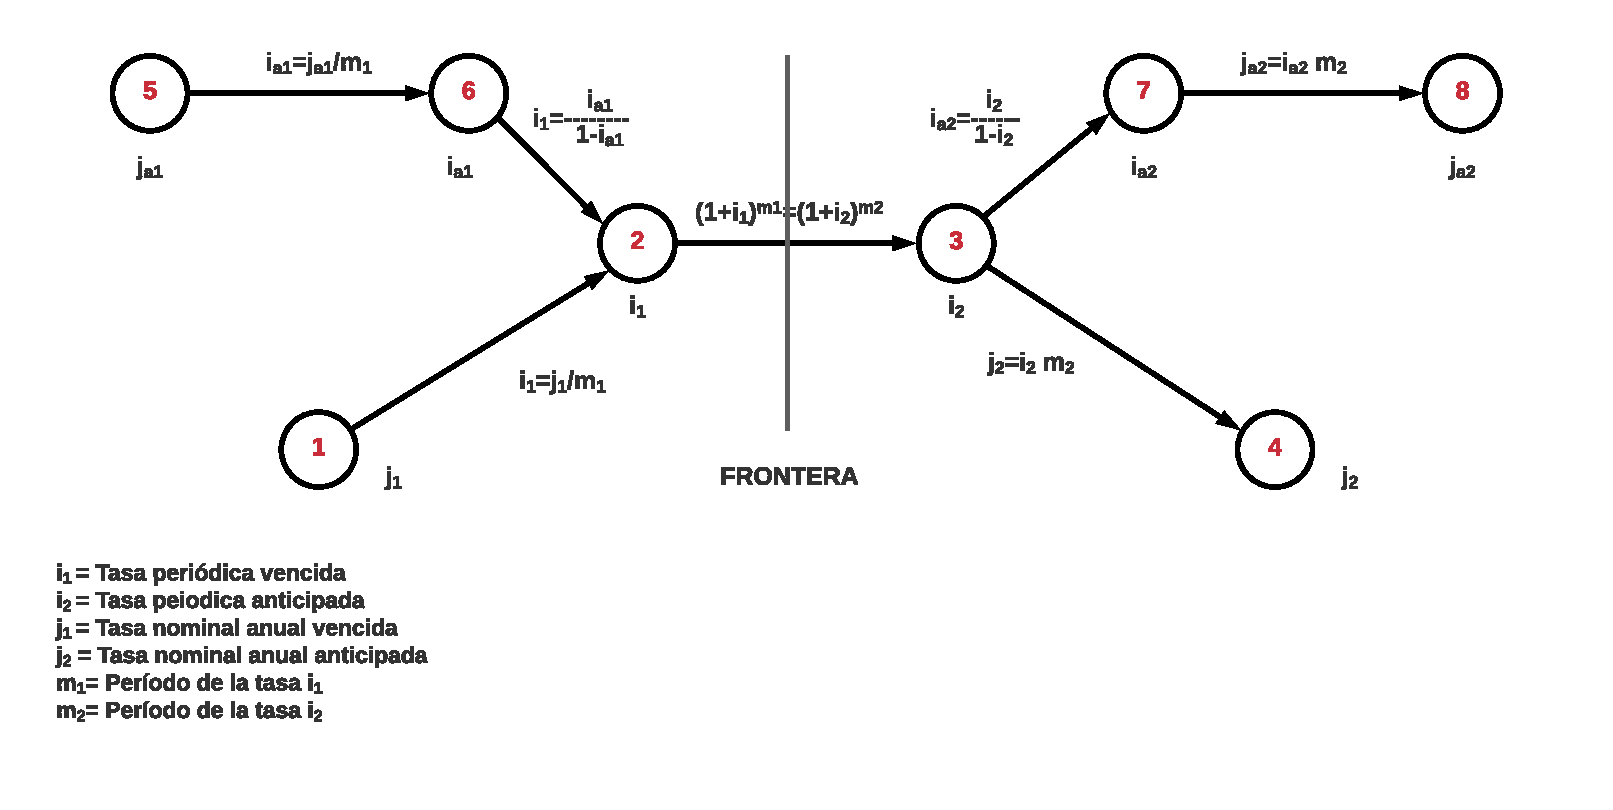
\includegraphics[trim=-5 -5 -5 -5 , scale=0.4]{2_Capitulo/img/ejemplos/6/Capitulo2Ejemplo6.pdf} }  \\ \hline
      
      %%%%%%%%%%%%% FIN INSERCIÓN DE IMAGEN
      %%%%%FIN FLUJO DE CAJA

      %%%%% INICIO DECLARACIÓN FORMULAS
      %%%%%%%%%%% INICIO TITULO
      \rowcolor[HTML]{FFB183}
      \multicolumn{3}{|c|}{\cellcolor[HTML]{FFB183}\textbf{4. Declaración de fórmulas}}                                                                                                                        \\ \hline
      %%%%%%%%%%% FIN TITULO
      %%%%%%%%%%% INICIO MATEMÁTICAS

      \multicolumn{2}{|c|}{ $ (1+i_{1})^{m_{1}}=(1+i_{2})^{m_{2}} \textit{ Equivalencia de tasas}$}      & $j_{a2}=i_{a2}\cdot m_{2} \textit{ Tasa nominal anual anticipada}$                                  \\ \multicolumn{2}{|c|}{$i_{a2} = \frac{i_{2}}{1+i_{2}} \textit{ Tasa periódica anticipada}$}           & \\ \hline
      %%%%%%%%%% FIN MATEMÁTICAS
      %%%%%% INICIO DESARROLLO MATEMÁTICO
      \rowcolor[HTML]{FFB183}
      %%%%%%%%%%INICIO TITULO
      \multicolumn{3}{|c|}{\cellcolor[HTML]{FFB183}\textbf{5. Desarrollo matemático}}                                                                                                                          \\ \hline
      %%%%%%%%%% FIN TITULO
      %%%%%%%%%% INICIO MATEMÁTICAS
      \multicolumn{2}{|c|}{$(1 + 0,02\%)^{12}= (1 + i_{2})^{2} $}                                    & {$j_{a2}=(11,20286178\% \textit{ pbv})(2\textit{ psv})$}                                                                  \\
      \multicolumn{2}{|c|}{$(1,02)^{6}-1=i_{2}$ }                                         & {$j_{a2} = 22,406\% \textit{ nasa}$}                                                                                                     \\
      \multicolumn{2}{|c|}{$i_{2}= 0,12616 \equiv 12,616\% \textit{ psv}$}                                      &                                                                                                     \\
      \multicolumn{2}{|c|}{$i_{a2}=\frac{0,126162419}{1+0,126162419}= 0,11203 \textit{ psa} \equiv 11,203\% \textit{ psa}$} &                                                                                                                                                                      \\ \hline

      %%%%%%%%%% FIN MATEMÁTICAS
      %%%%%% FIN DESARROLLO MATEMÁTICO
      %%%%%% INICIO RESPUESTA
      \rowcolor[HTML]{FFB183}
      %%%%%%%%%%INICIO TITULO
      \multicolumn{3}{|c|}{\cellcolor[HTML]{FFB183}\textbf{6. Respuesta}}                                                                                                                                      \\ \hline
      %%%%%%%%%% FIN TITULO
      %%%%%%%%%% INICIO RESPUESTA MATEMÁTICA
      \multicolumn{3}{|c|}{
         \begin{minipage}[t][0.03\textheight][c]{0.8\columnwidth}
            \centering
            ${j_{a2} = 22,406\% nasa}$
         \end{minipage}
      }   

                                                \\ \hline
      
      %%%%%%%%%% FIN MATEMÁTICAS
      %%%%%% FIN RESPUESTA
   \end{longtable}
   %Se crean dos lineas en blanco para que no quede el siguiente texto tan pegado
   %\newline \newline %USARLO SI CREES QUE ES NECESARIO
\end{center}
%%%%%%%%%%%%%%%%%%% FIN EJERCICIO 9.d  %%%%%%%%%%%%%%%%%%%%%%%%%%%%%%
%%%%%%%%%%%%%%%%%%%%%%%%%%FIN EJERCICIO 9 %%%%%%%%%%%%%%%%%%%%%%%%%%%

%%%%%%%%%%%%%%%%%%% EJERCICIO 10 %%%%%%
\textbf{Ejemplo 10}\\
¿Cuál es la tasa nominal anual (150 días) vencido equivalente a una tasa del 24\% 
periódica (200 días) anticipada? Asumir el año de 365 días.\\
%\newpage %USAR SOLO SI EL SOLUCIÓN QUEDA SOLO Y ES NECESARIO BAJARLO A LA SIGUIENTE PAGINA
\hfill
\textbf{Solución }\\
%La tabla ira centrada
\begin{center}
  \renewcommand{\arraystretch}{1.5}% Margenes de las celdas
  %Creación de la cuadricula de 2 columnas
  \begin{longtable}[H]{|c|c|c|}
    %Creamos una linea horizontal
    \hline
    %Definimos el color de la primera fila
    \rowcolor[HTML]{FFB183}
    %%%%% INICIO ASIGNACIÓN PERíODO FOCAL %%%%%%%
    %%%%%%%%%% INICIO TITULO

    %Lo que se hace aquí es mezclar las 3 columnas en una sola
      \multicolumn{3}{|c|}{\cellcolor[HTML]{FFB183}\textbf{1. Asignación período focal}}                                                                                                        \\ \hline
      \multicolumn{3}{|c|}{$pf= \textit{No aplica}$}                                                                                                                                              
      \\ \hline

    %%%%%%%%%% FIN TITULO
    %%%%% INICIO DECLARACIÓN DE VARIABLES %%%%%%%
    %%%%%%%%%% INICIO TITULO
    %Lo que se hace aquí es mezclar las 3 columnas en una sola
    \multicolumn{3}{|c|}{\cellcolor[HTML]{FFB183}\textbf{2. Declaración de variables}}                                                                 \\ \hline
    %%%%%%%%%% FIN TITULO
    %%%%%%%%%% INICIO DE MATEMÁTICAS
    %Cada & hace referencia al paso de la siguiente columna
    $j_{a1} = 24\% \textit{ na(200)da}$  &  $m_{1} =\frac{365días}{200días}= 1,82 \textit{ p(200)da}$  &  $i_{2} = ?\% \textit{ p(150)dv} $ \\ 
    
    $i_{a1}= 0,1319 \textit{ p(200)da} $ & $m_{2} = \frac{365días}{150días} = 2,43 \textit{ p(150)dv}$ & $j_{2} = ?\% \textit{ na(150)dv} $    \\                                                                                                     \hline
    %%%%%%%%%% FIN DE MATEMÁTICAS
    %%%%% FIN DECLARACIÓN DE VARIABLES

    %%%%% INICIO FLUJO DE CAJA
    \rowcolor[HTML]{FFB183}
    \multicolumn{3}{|c|}{\cellcolor[HTML]{FFB183}\textbf{3. Diagrama de equivalencia de tasas}}                                                        \\ \hline
    %Mezclamos 3 columnas y pondremos el dibujo
    %%%%%%%%%%%%% INSERCIÓN DE LA IMAGEN
    %Deberán descargar las imágenes respectivas del drive y pegarlas en la carpeta
    %n_capitulo/img/ejemplos/1/capitulo1ejemplo1.pdf  (el /1/ es el numero del ejemplo)

    \multicolumn{3}{|c|}{ 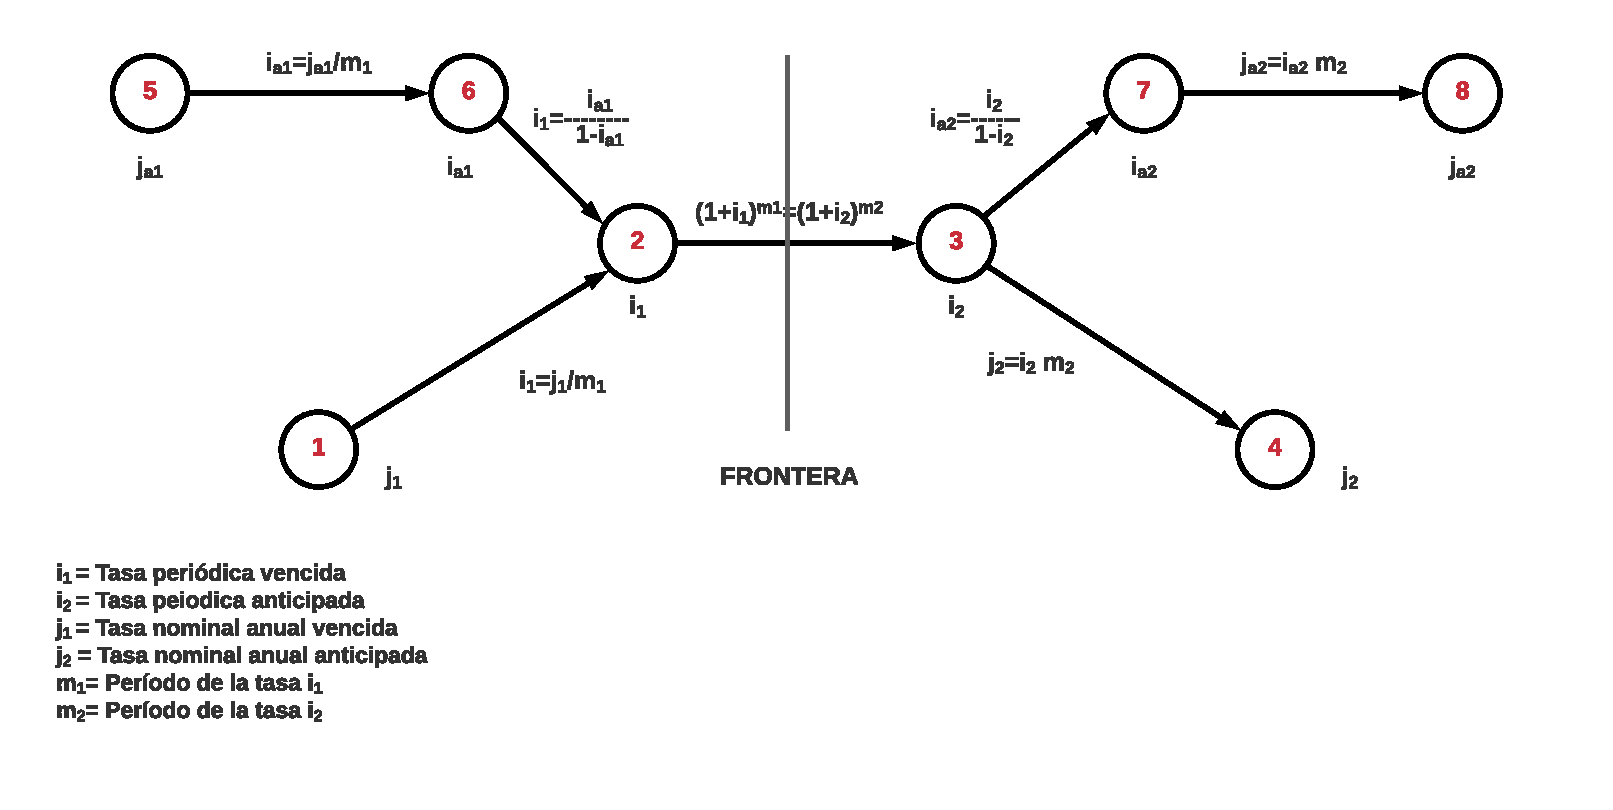
\includegraphics[trim=-5 -5 -5 -5 , scale=0.4]{2_Capitulo/img/ejemplos/6/Capitulo2Ejemplo6.pdf} } \\ \hline
    
    %%%%%%%%%%%%% FIN INSERCIÓN DE IMAGEN
    %%%%%FIN FLUJO DE CAJA

    %%%%% INICIO DECLARACIÓN FORMULAS
    %%%%%%%%%%% INICIO TITULO
    \rowcolor[HTML]{FFB183}
    \multicolumn{3}{|c|}{\cellcolor[HTML]{FFB183}\textbf{4. Declaración de fórmulas}}                                                                  \\ \hline
    %%%%%%%%%%% FIN TITULO
    %%%%%%%%%%% INICIO MATEMÁTICAS

    \multicolumn{2}{|c|} {$i_{1} = \frac{i_{1}}{1-{i_{a1}}} \textit{ Tasa periódica vencida }$} & {{\raggedleft  $j_{2}=i_{2}\cdot m_{2} \textit{ Tasa nominal anual vencida }$}} \\
    \multicolumn{2}{|c|} {$(1+i_{1})^{m_{1}}=(1+i_{2})^{m_{2}} \textit{ Equivalencia de tasas}$ }  & {$i_{a1} = \frac{j_{a1}}{m_{1}} \textit{ Tasa periódica anticipada}$}     \\ \hline
    %%%%%%%%%% FIN MATEMÁTICAS
    %%%%%% INICIO DESARROLLO MATEMÁTICO
    \rowcolor[HTML]{FFB183}
    %%%%%%%%%%INICIO TITULO
    \multicolumn{3}{|c|}{\cellcolor[HTML]{FFB183}\textbf{5. Desarrollo matemático}}                                                                    \\ \hline
    %%%%%%%%%% FIN TITULO
    %%%%%%%%%% INICIO MATEMÁTICAS
    \multicolumn{2}{|c|} {$i_{1} = \frac{0.1319}{1-0,1319} = 0,152 \textit{p(200)dv}$}   &  {$j_{2}=(11,18\% \textit{ p(150)dv})(2,43\textit{ p(150)dv})$}                            \\
    \multicolumn{2}{|c|} {$(1 + 0,152)^{1,82}= (1 + i_{2})^{2,43} $}  &  {\textit{$j_{2} = 27,17\% \textit{ na(150)dv}$}}                                                                          \\
    \multicolumn{2}{|c|} {$(1,152)^{\frac{1,82}{2,43}}-1=i_{2}$}  &                                                                            \\
    \multicolumn{2}{|c|} {$i_{2}=0,1118 \textit{ p(150)dv} \equiv 11,18\% \textit{ p(150)dv}$}                                   &                                                                                                   \\ 
    \hline
    %%%%%%%%%% FIN MATEMÁTICAS
    %%%%%% FIN DESARROLLO MATEMÁTICO
    %%%%%% INICIO RESPUESTA
    \rowcolor[HTML]{FFB183}
    %%%%%%%%%%INICIO TITULO
    \multicolumn{3}{|c|}{\cellcolor[HTML]{FFB183}\textbf{6. Respuesta}}                                                                                \\ \hline
    %%%%%%%%%% FIN TITULO
    %%%%%%%%%% INICIO RESPUESTA MATEMÁTICA
    \multicolumn{3}{|c|}{
         \begin{minipage}[t][0.03\textheight][c]{0.8\columnwidth}
            \centering
             ${j_{2} = 27,17\% na(150)dv}$
         \end{minipage}
      }  
    \\ \hline
    %%%%%%%%%% FIN MATEMÁTICAS
    %%%%%% FIN RESPUESTA
  \end{longtable}
  %Se crean dos lineas en blanco para que no quede el siguiente texto tan pegado
  %\newline \newline %USARLO SI CREES QUE ES NECESARIO
\end{center}
%%%%%%%%%%%%%%%%%%% FIN EJERCICIO 10  %%%%%%%%%%%%%%%%%%%%%%%%%%%%%%


\section{Ecuaciones de equivalencia de flujos}
Es muy frecuente cambiar una o varias obligaciones por otra u otras nuevas obligaciones. La solución de este problema es elemental y para solucionarlo es necesario usar la ecuación de equivalencia de flujos, que es una igualdad de valores ubicados en una sola fecha denominada período focal.\\
La período focal se representa gráficamente por una línea a trazos y por las letras pf y es la fecha en que debe hacerse la igualdad entre ingresos (flujos positivos) y egresos (flujos negativos) . La ubicación de la período focal no altera la respuesta final, por tal motivo se deja a libre elección de la persona que va a resolver el problema.\\
El principio fundamental de una ecuación de valor, que viene a ser el mismo principio fundamental de las finanzas, establece que la sumatoria de los ingresos debe ser igual a la sumatoria de los egresos ubicados ambos en la período focal, esto es:

\begin{center}
   $\sum ingresos = \sum egresos(en\ la\ pf)$\\
\end{center}
Naturalmente, para el traslado de cada una de las cantidades a la período focal, debe hacerse usando la fórmula de valor futuro.\\
El enunciado de una ecuación de equivalencia también puede ser expresado así:

\begin{center}
   $\sum deudas = \sum pagos(en\ la\ pf)$\\
\end{center}

Mirando un balance el principio puede ser expresado así:\\

\begin{center}
   $\sum activos = \sum pasivos + capital(en\ la\ pf)$\\
\end{center}

Como en cualquier proyecto, los ingresos se representan por flechas hacia arriba y los egresos por flechas hacia abajo, entonces, mirando la gráfica de flujo de caja podemos expresar el principio fundamental de una ecuación de equivalencia de flujos de esta otra forma:\\

\begin{center}
   $\sum de\ lo\ que\ $\textit{está}$\ para\ arriba = \sum de\ lo\ que\ $\textit{está}$\ para\ abajo(en\ la\ pf)$\\
\end{center}

La sumatoria de los ingresos en pesos de hoy menos la sumatoria de los egresos en pesos de hoy recibe el nombre de valor presente neto (VPN) o valor actual neto.\\
La tasa a la cual la sumatoria de los ingresos (VPN) es igual a la sumatoria de los egresos (en la período focal) se denomina tasa interna de retorno (TIR).\\
En el capítulo posterior analizaremos con más detalle los conceptos de VPN y TIR, estos conceptos son de suma importancia en la evaluación de proyectos.\\

\textbf{Ejemplo 11}

Una persona se comprometió a pagar 250.000 COP en 3 meses, 300.000 COP en 8 meses y 130.000 COP en 15 meses. Ante la dificultad de cumplir con las obligaciones tal como están pactadas solicita una nueva forma de pago así: 60.000 COP hoy, 500.000 COP en 12 meses y el saldo en 18 meses. Suponiendo que la tasa de interés de oportunidad es del 36 \% nominal anual mes vencido, determinar el valor del saldo.
\\

\begin{table}
  \centering
  \resizebox{\columnwidth}{!}{%
  \begin{tabular}{|cll|}
  \hline
  \multicolumn{3}{|c|}{\cellcolor[HTML]{FFB183}\textbf{1. Asignación período focal}}  \\ \hline
  \multicolumn{3}{|c|}{pf = 8pmv}                                                     \\ \hline
  \multicolumn{3}{|c|}{\cellcolor[HTML]{FFB183}\textbf{2. Declaración de variables}}  \\ \hline
  \multicolumn{3}{|c|}{\cellcolor[HTML]{FFB183}\textbf{2.1 Deuda inicial}}            \\ \hline
  \multicolumn{1}{|l|}{\begin{tabular}[c]{@{}l@{}}$P_1 = 250.000$ COP\\ $n_1 = 5pmv$\end{tabular}} &
    \multicolumn{1}{l|}{\begin{tabular}[c]{@{}l@{}}$P_2 = 300.000$ COP\\ $n_2 = 0 pmv$\end{tabular}} &
    \begin{tabular}[c]{@{}l@{}}$F_3 = 130.000$ COP\\ $n_3 = -7pmv$\end{tabular} \\ \hline
  \multicolumn{3}{|c|}{$j = 36\%$ namv $\equiv i = 3\%$ pmv}                               \\ \hline
  \multicolumn{3}{|c|}{\cellcolor[HTML]{FFB183}\textbf{2.2 Deuda equivalente}}        \\ \hline
  \multicolumn{1}{|l|}{\begin{tabular}[c]{@{}l@{}}$P_4 = 60.000$ COP\\ $n_4 = 8$ pmv\end{tabular}} &
    \multicolumn{1}{l|}{\begin{tabular}[c]{@{}l@{}}$F_5 = 500.000$ COP\\ $n_5 = -4$ pmv\end{tabular}} &
    \begin{tabular}[c]{@{}l@{}}$F_6 = ?$ COP\\ $n_6 = −10$ pmv\end{tabular} \\ \hline
  \multicolumn{3}{|c|}{$j = 36\%$ namv $ \equiv i = 3\%$ pmv}                               \\ \hline
  \multicolumn{3}{|c|}{\cellcolor[HTML]{FFB183}\textbf{3. Diagrama de flujo de caja}} \\ \hline
  \multicolumn{3}{|c|}{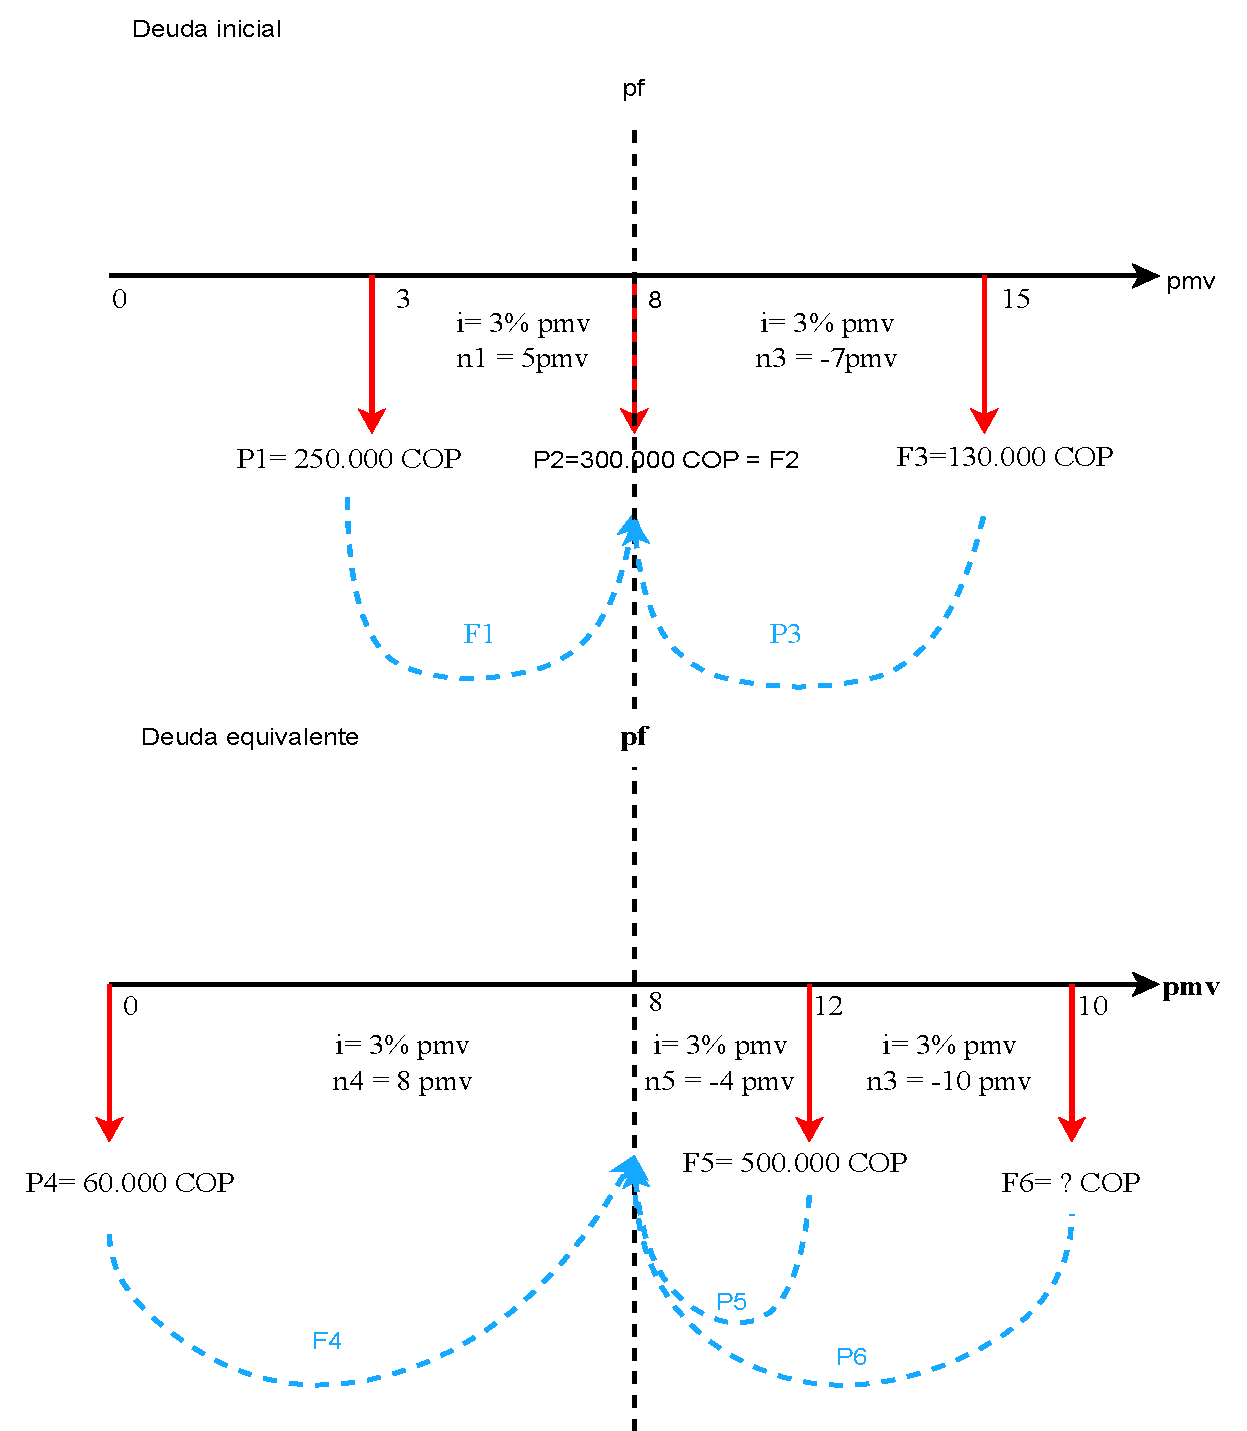
\includegraphics[trim=-5 -5 -5 -5 , scale=0.8]{2_Capitulo/img/ejemplos/11/Ejemplo 11ver.pdf} } \\ \hline
  \multicolumn{3}{|c|}{\cellcolor[HTML]{FFB183}\textbf{4. Declaración de fórmulas}}   \\ \hline
  \multicolumn{3}{|l|}{\begin{tabular}[c]{@{}l@{}}
    $F_1 + P_2 + P_3 = F_4 + P_5 + P_6$ Ecuación de equivalencia\\ 
    $F = P(1+i)^n$ Valor futuro\\ 
    $P = F(1 + i)^{−n}$ Valor presente (en pf)\end{tabular}} \\ \hline
  \multicolumn{3}{|c|}{\cellcolor[HTML]{FFB183}\textbf{5. Desarrollo matemático}}     \\ \hline
  \multicolumn{3}{|c|}{$250.000 $ COP $ (1+0.03)^{5}$$+ 300.000$ COP $(1+0.03)^0$$+ 130.000$ COP $(1+0.03)^{-7}$} \\
  \multicolumn{3}{|c|}{$=$} \\
  \multicolumn{3}{|c|}{$60.000$ COP $(1+0.03)^{8}$$+ 500.000$ COP $(1+0.03)^{-4}$$+ F_6$ COP $(1+0.03)^{-10}$} \\ \hline
  \multicolumn{3}{|c|}{\cellcolor[HTML]{FFB183}\textbf{6. Respuesta}}                 \\ \hline
  \multicolumn{3}{|c|}{
  {$F_6$ =235.549,16 COP Valor del saldo}}                            \\ \hline
  \end{tabular}%
  }
\end{table}
\pagebreak

%%%%%%%%%%%%%%%%%%% EJERCICIO 12 %%%%%%
\textbf{Ejemplo 12}\\
Una deuda de 15.000 COP fue contraída hace 2 meses con fecha de vencimiento en 4
meses a partir de hoy, esta posee un interés del 24\% nominal anual trimestre vencido y
otra deuda de 25.000 COP contraída hace un mes con vencimiento de 8 meses a partir de hoy
e intereses del 28\% nominal anual semestre vencido. Se van a cancelar las deudas
mediante dos pagos de igual valor, efectuados el primero el día de hoy y el segundo en 6
meses. Con un interés del 30\% nominal anual mes vencido y el segundo en 6 meses,
determinar el valor de los pagos.\\ \\
%\newpage %USAR SOLO SI EL SOLUCIÓN QUEDA SOLO Y ES NECESARIO BAJARLO A LA SIGUIENTE PAGINA
\textbf{Solución.}\\
%La tabla ira centrada
\begin{center}
  \renewcommand{\arraystretch}{1.5}% Margenes de las celdas
  %Creación de la cuadricula de 3 columnas
  \begin{longtable}[H]{|c|c|c|}
    %Creamos una linea horizontal
    \hline
    %Definimos el color de la primera fila
    \rowcolor[HTML]{FFB183}
    %%%%% INICIO ASIGNACIÓN PERíODO FOCAL %%%%%%%
    %%%%%%%%%% INICIO TITULO
    %Lo que se hace aquí es mezclar las 3 columnas en una sola
    \multicolumn{3}{|c|}{\cellcolor[HTML]{FFB183}\textbf{1. Asignación período focal}}                                                                                              \\ \hline
    \multicolumn{3}{|c|}{\textbf{ $pf = \textit{ período focal: 6 pmv} $}}                                                                                                          \\ \hline
    %%%%%%%%%% FIN TITULO
    %%%%% INICIO DECLARACIÓN DE VARIABLES %%%%%%%
    %%%%%%%%%% INICIO TITULO
    %Lo que se hace aquí es mezclar las 3 columnas en una sola
    \multicolumn{3}{|c|}{\cellcolor[HTML]{FFB183}\textbf{2. Declaración de variables}}                                                                                              \\ \hline
    %%%%%%%%%% FIN TITULO
    %%%%%%%%%% INICIO DE MATEMÁTICAS
    %Cada & hace referencia al paso de la siguiente columna
    Deuda 1:                                               & Deuda2:                                                                               & Deuda equivalente              \\
    $j_{1} = 24\% \textit{ natv} $                         & $j_{2} = 28\% \textit{ nasv} $                                                        & $j_{3} = 30\% \textit{ namv} $ \\
    $i_{1} = 6\% \textit{ ptv} $                           & $i_{2} = 14\% \textit{ psv} $                                                         & $i_{3} = 2,5\% \textit{ pmv} $ \\
    $n_ {1} = 2 \textit{ ptv}  $                           & $n_ {2} = 1,5 \textit{ psv} $                                                         & $n_ {3} = 6 \textit{ pmv}  $   \\
    $P_{1} =    15.000 $ COP                               & $P_{2} = 25.000 $ COP                                                              & $F_{5} = F_{6} =  ? $ COP      \\
    $F_{1} =   ? $ COP
    & $F_{2} =   ? $ COP   
    &
    \\
    $F_{3} = ? $ COP
    & $P_{4} = ? $ COP
    &
    \\ \hline


    %%%%%%%%%% FIN DE MATEMÁTICAS
    %%%%% FIN DECLARACIÓN DE VARIABLES


    %%%%% INICIO FLUJO DE CAJA
    \rowcolor[HTML]{FFB183}
    \multicolumn{3}{|c|}{\cellcolor[HTML]{FFB183}\textbf{3. Diagrama de flujo de caja}}                                                                                             \\ \hline
    %Mezclamos 3 columnas y pondremos el dibujo
    %%%%%%%%%%%%% INSERCIÓN DE LA IMAGEN
    %Deberán descargar las imágenes respectivas del drive y pegarlas en la carpeta
    %n_capitulo/img/ejemplos/1/capitulo1ejemplo1.pdf  (el /1/ es el numero del ejemplo)
    \multicolumn{3}{|c|}{ 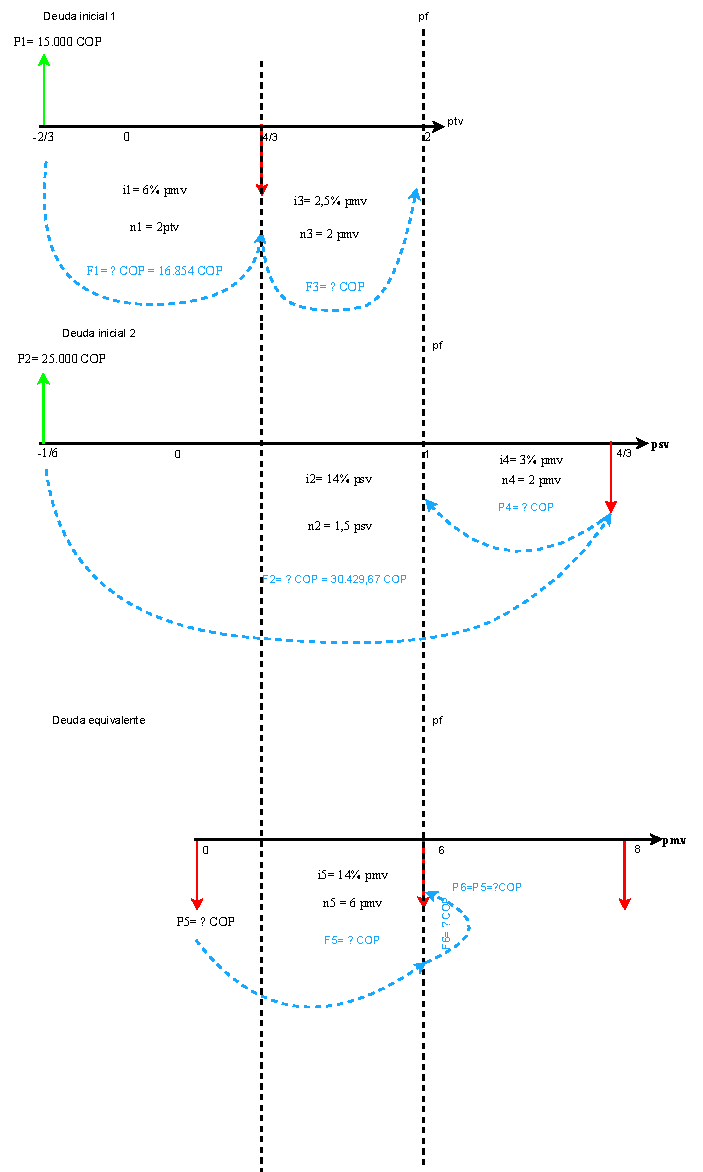
\includegraphics[trim=-5 -5 -5 -5 , scale=0.84]{2_Capitulo/img/ejemplos/14/Ejemplo 12Ver.pdf}}
    \\ \hline
    %%%%%%%%%%%%% FIN INSERCIÓN DE IMAGEN
    %%%%%FIN FLUJO DE CAJA



    %%%%% INICIO DECLARACIÓN FORMULAS
    %%%%%%%%%%% INICIO TITULO
    \rowcolor[HTML]{FFB183}
    \multicolumn{3}{|c|}{\cellcolor[HTML]{FFB183}\textbf{4. Declaración de fórmulas}}                                                                                               \\ \hline
    %%%%%%%%%%% FIN TITULO
    %%%%%%%%%%% INICIO MATEMÁTICAS

    $F = P(1+i)^n \hspace{0.3cm} \textit{Valor futuro}$
    & \multicolumn{2}{c|}{$F_{3}+P_{4}=F_{5}+P_{6}\hspace{0.3cm}\textit{Ecuación de valor}$}
    \\
    $j=i*m\hspace{0.3cm}\textit{Tasa periódica anualizada}$
    & \multicolumn{2}{c|}{$P = F(1+i)^{-n} \hspace{0.3cm} \textit{Valor presente}$ }
 
    \\ \hline

    %%%%%%%%%% FIN MATEMÁTICAS
    %%%%%% INICIO DESARROLLO MATEMÁTICO
    \rowcolor[HTML]{FFB183}
    %%%%%%%%%%INICIO TITULO
    \multicolumn{3}{|c|}{\cellcolor[HTML]{FFB183}\textbf{5. Desarrollo matemático}}                                                                                                 \\ \hline
    %%%%%%%%%% FIN TITULO
    %%%%%%%%%% INICIO MATEMÁTICAS
    $F_{1}= 15.000$ COP $ (1 + 0,06)^{2}=  16.854$ COP    & \multicolumn{2}{|c|}{$16.854$ COP$ (1+0,025)^{2}$}
    \\
    $F_{2}= 25.000$ COP $ (1 + 0,14)^{1,5}= 30.429,67$ COP & \multicolumn{2}{|c|}{$+ 30.429,67$ COP $ (1+0,025)^{-2}$} 
    \\
    &
    \multicolumn{2}{|c|}{$  = P_{5}$ COP $(1+0,025)^{6} + P_{5}$ COP}
    \\
    &
    \multicolumn{2}{|c|}{$P_{5}=21.609,84 $ COP}
    
    \\ \hline


    %%%%%%%%%% FIN MATEMÁTICAS
    %%%%%% FIN DESARROLLO MATEMÁTICO
    %%%%%% INICIO RESPUESTA
    \rowcolor[HTML]{FFB183}
    %%%%%%%%%%INICIO TITULO
    \multicolumn{3}{|c|}{\cellcolor[HTML]{FFB183}\textbf{6. Respuesta}}                                                                                                             \\ \hline
    %%%%%%%%%% FIN TITULO
    %%%%%%%%%% INICIO RESPUESTA MATEMÁTICA
    \multicolumn{3}{|c|}{{$F_{5}$ = $F_{6}$ = 21.609,84 COP.}}                                                                                                                                                                               \\ \hline


    %%%%%%%%%% FIN MATEMÁTICAS
    %%%%%% FIN RESPUESTA
  \end{longtable}
  %Se crean dos lineas en blanco para que no quede el siguiente texto tan pegado
  %\newline \newline %USARLO SI CREES QUE ES NECESARIO
\end{center}
%%%%%%%%%%%%%%%%%%%%%%%%%%FIN EJERCICIO 12 %%%%%%%%%%%%%%%%%%%%%%%%%%%
\setlength{\parskip}{\baselineskip}

%%%%%%%%%%%%%%%%%%% EJERCICIO 13 %%%%%%

\textbf{Ejemplo 13}\\
Una persona debe pagar  10.000 COP con vencimiento en 3 meses, 15.000 COP a 10 meses y 20.000 COP con vencimiento en un año. Si hace un pago único de 45.000 COP, hallar la fecha en que debe hacerse, suponga una tasa del 18\% nominal anual mes vencido. Si consideramos la período focal (pf) en el período mes vencido 0:\\ \\
%\newpage %USAR SOLO SI EL SOLUCIÓN QUEDA SOLO Y ES NECESARIO BAJARLO A LA SIGUIENTE PAGINA
\textbf{Solución.}
%La tabla ira centrada
\begin{center}
  \renewcommand{\arraystretch}{1.5}% Margenes de las celdas
  %Creación de la cuadricula de 3 columnas
  \begin{longtable}[H]{|C{0.3\linewidth}|C{0.3\linewidth}|C{0.3\linewidth}|}
    %Creamos una linea horizontal
    \hline
    %Definimos el color de la primera fila
    \rowcolor[HTML]{FFB183}
    %%%%% INICIO ASIGNACIÓN PERíODO FOCAL %%%%%%%
    %%%%%%%%%% INICIO TITULO
    %Lo que se hace aquí es mezclar las 3 columnas en una sola
    \multicolumn{3}{|c|}{\cellcolor[HTML]{FFB183}\textbf{1. Asignación período focal}}                                                                                          \\ \hline
    \multicolumn{3}{|c|}{\textbf{ $pf = \textit{ período focal: 0 pmv} $}}                                                                                                      \\ \hline
    %%%%%%%%%% FIN TITULO
    %%%%% INICIO DECLARACIÓN DE VARIABLES %%%%%%%
    %%%%%%%%%% INICIO TITULO
    %Lo que se hace aquí es mezclar las 3 columnas en una sola
    \multicolumn{3}{|c|}{\cellcolor[HTML]{FFB183}\textbf{2. Declaración de variables}}                                                                                          \\ \hline
    %%%%%%%%%% FIN TITULO
    %%%%%%%%%% INICIO DE MATEMÁTICAS
    %Cada & hace referencia al paso de la siguiente columna

    $j = 18\% \textit{ namv} $
    & $F_{1} =10.000$ COP
    & $n_{1} = -3 \textit{ pmv} $    
    \\
    $i = 1,5\% \textit{ pmv} $ 
    & $F_{2} = 15.000$ COP              
    & $n_{2} = -10 \textit{ pmv} $    
    \\
    & $F_{3} =20.000$ COP
    & $n_{3}= -12 \textit{ pmv}  $    
    \\
    & $F_{4} =45.000$ COP
    & $n_{4} = 12-x \textit{ pmv} $ 
    \\
    \hline

    %%%%%%%%%% FIN DE MATEMÁTICAS
    %%%%% FIN DECLARACIÓN DE VARIABLES


    %%%%% INICIO FLUJO DE CAJA
    \rowcolor[HTML]{FFB183}
    \multicolumn{3}{|c|}{\cellcolor[HTML]{FFB183}\textbf{3. Diagrama de flujo de caja}}                                                                                         \\ \hline
    %Mezclamos 3 columnas y pondremos el dibujo
    %%%%%%%%%%%%% INSERCIÓN DE LA IMAGEN
    %Deberán descargar las imágenes respectivas del drive y pegarlas en la carpeta
    %n_capitulo/img/ejemplos/1/capitulo1ejemplo1.pdf  (el /1/ es el numero del ejemplo)
    \multicolumn{3}{|c|}{ 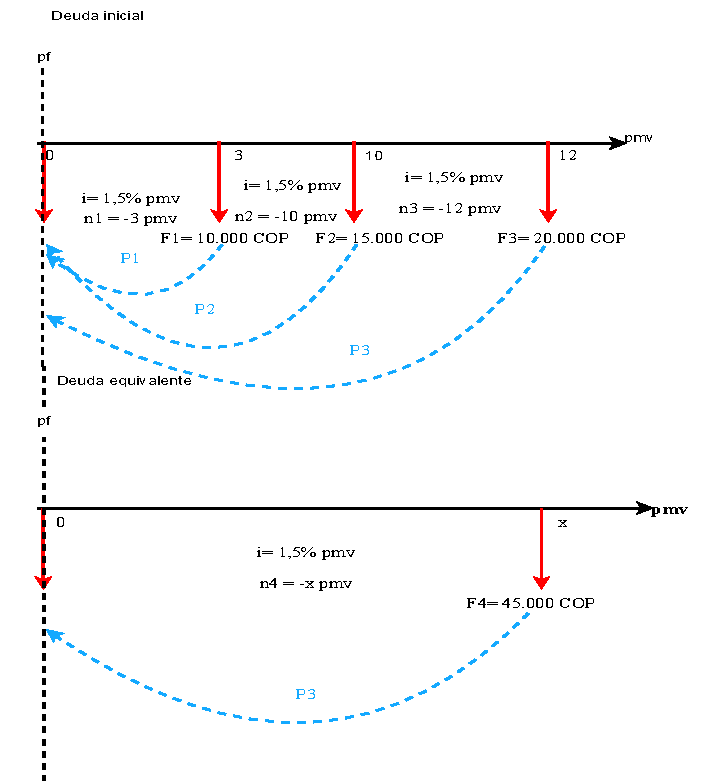
\includegraphics[trim=-5 -5 -5 -5 , scale=0.65]{2_Capitulo/img/ejemplos/14/Ejemplo 13Ver.pdf} }
    \\ \hline
    %%%%%%%%%%%%% FIN INSERCIÓN DE IMAGEN
    %%%%%FIN FLUJO DE CAJA



    %%%%% INICIO DECLARACIÓN FORMULAS
    %%%%%%%%%%% INICIO TITULO
    \rowcolor[HTML]{FFB183}
    \multicolumn{3}{|c|}{\cellcolor[HTML]{FFB183}\textbf{4. Declaración de fórmulas}}                                                                                           \\ \hline
    %%%%%%%%%%% FIN TITULO
    %%%%%%%%%%% INICIO MATEMÁTICAS

    $P_{1} + P_{2} + P_{3} = P_{4} \textit{ Ecuación de eqv.}$ & \multicolumn{2}{c|}{$P = F(1+i)^{-n} \hspace{0.3cm} \textit{Valor presente}$ }
    \\
    & \multicolumn{2}{c|}{$F = P(1+i)^n \hspace{0.3cm} \textit{Valor futuro}$}\\
    \hline
    %%%%%%%%%% FIN MATEMÁTICAS
    %%%%%% INICIO DESARROLLO MATEMÁTICO
    \rowcolor[HTML]{FFB183}
    %%%%%%%%%%INICIO TITULO
    \multicolumn{3}{|c|}{\cellcolor[HTML]{FFB183}\textbf{5. Desarrollo matemático}}                                                                                             \\ \hline
    %%%%%%%%%% FIN TITULO
    %%%%%%%%%% INICIO MATEMÁTICAS

    \multicolumn{3}{|C{\linewidth}|}{$10.000$ COP $( 1 + 0,015)^{-3}$ + $15.000$ COP $( 1 + 0,015)^{-10}$}
    \\
    \multicolumn{3}{|C{\linewidth}|}{+ $20.000$ COP $( 1 + 0,015)^{-12} = 45.000$ COP $( 1 + 0,015)^{-x} $}
    \\
    \multicolumn{3}{|C{\linewidth}|}{$ ln(30.609.007391/45.000)= (-x)ln(1,015)  $ }                                                                                            \\ \hline


    %%%%%%%%%% FIN MATEMÁTICAS
    %%%%%% FIN DESARROLLO MATEMÁTICO
    %%%%%% INICIO RESPUESTA
    \rowcolor[HTML]{FFB183}
    %%%%%%%%%%INICIO TITULO
    \multicolumn{3}{|c|}{\cellcolor[HTML]{FFB183}\textbf{6. Respuesta}}                                                                                                         \\ \hline
    %%%%%%%%%% FIN TITULO
    %%%%%%%%%% INICIO RESPUESTA MATEMÁTICA
    \multicolumn{3}{|c|}{

      \begin{minipage}[t][0.07\textheight][c]{0.8\columnwidth}
       \centering
        $n_{4} = 9,24059 \textit{ pmv} \approx t = 9 \textit{ meses y }  7 \textit{ dias.} $
      \end{minipage}
    }                                                                                                                                                                           \\ \hline


    %%%%%%%%%% FIN MATEMÁTICAS
    %%%%%% FIN RESPUESTA
  \end{longtable}
  %Se crean dos lineas en blanco para que no quede el siguiente texto tan pegado
  %\newline \newline %USARLO SI CREES QUE ES NECESARIO
\end{center}
%%%%%%%%%%%%%%%%%%%%%%%%%%FIN EJERCICIO 13 %%%%%%%%%%%%%%%%%%%%%%%%%%%

%%%%%%%%%%%%%%%%%%%% EJERCICIO 14 %%%%%%

\textbf{Ejemplo 14}\\
Una persona debe pagar 70.000 COP en 3 meses y 85.000 COP en 8 meses; ante la imposibilidad de cancelar las deudas en las fechas previstas le ofrece al acreedor que le cancelara 50.000 COP en 4 meses y 130.000 COP en 12 meses. Si el acreedor acepta esta nueva forma de pago ¿Qué tasa de interés periódica mes vencido estará pagando?.\\ \\
\setlength{\parskip}{-1mm}
%\newpage %USAR SOLO SI EL SOLUCIÓN QUEDA SOLO Y ES NECESARIO BAJARLO A LA SIGUIENTE PAGINA
\textbf{Solución.}
%La tabla ira centrada

\begin{center}
  \renewcommand{\arraystretch}{1.5}% Margenes de las celdas
  %Creación de la cuadricula de 3 columnas
  \begin{longtable}[H]{|c|c|c|}
    %Creamos una linea horizontal
    \hline
    %Definimos el color de la primera fila
    \rowcolor[HTML]{FFB183}
    %%%%% INICIO ASIGNACIÓN PERíODO FOCAL %%%%%%%
    %%%%%%%%%% INICIO TITULO
    %Lo que se hace aquí es mezclar las 3 columnas en una sola
    \multicolumn{3}{|c|}{\cellcolor[HTML]{FFB183}\textbf{1. Asignación período focal}}                                                      \\ \hline
    \multicolumn{3}{|c|}{\textbf{ $pf = \textit{ período focal: 0 pmv} $}}                                                                  \\ \hline
    %%%%%%%%%% FIN TITULO
    %%%%% INICIO DECLARACIÓN DE VARIABLES %%%%%%%
    %%%%%%%%%% INICIO TITULO
    %Lo que se hace aquí es mezclar las 3 columnas en una sola
    \multicolumn{3}{|c|}{\cellcolor[HTML]{FFB183}\textbf{2. Declaración de variables}}                                                      \\ \hline
    %%%%%%%%%% FIN TITULO
    %%%%%%%%%% INICIO DE MATEMÁTICAS
    %Cada & hace referencia al paso de la siguiente columna
    $F_{1} =    70.000  $ COP & $F_{3} =    50.000 $  COP  & $n_ {2} = -8 \textit{ pmv}  $                                                  \\
    $F_{2} =    85.000  $ COP & $F_{4} =    130.000  $ COP & $n_ {3} = -4 \textit{ pmv}   $                                                 \\
    $i = ?\%  $               & $n_{1} = -3 \textit{ pmv}  $ & $n_ {4} = -12 \textit{ pmv}  $                                                 \\ \hline

    %%%%%%%%%% FIN DE MATEMÁTICAS
    %%%%% FIN DECLARACIÓN DE VARIABLES


    %%%%% INICIO FLUJO DE CAJA
    \rowcolor[HTML]{FFB183}
    \multicolumn{3}{|c|}{\cellcolor[HTML]{FFB183}\textbf{3. Diagrama de flujo de caja}}                                                     \\ \hline
    %Mezclamos 3 columnas y pondremos el dibujo
    %%%%%%%%%%%%% INSERCIÓN DE LA IMAGEN
    %Deberán descargar las imágenes respectivas del drive y pegarlas en la carpeta
    %n_capitulo/img/ejemplos/1/capitulo1ejemplo1.pdf  (el /1/ es el numero del ejemplo)
    \multicolumn{3}{|c|}{ 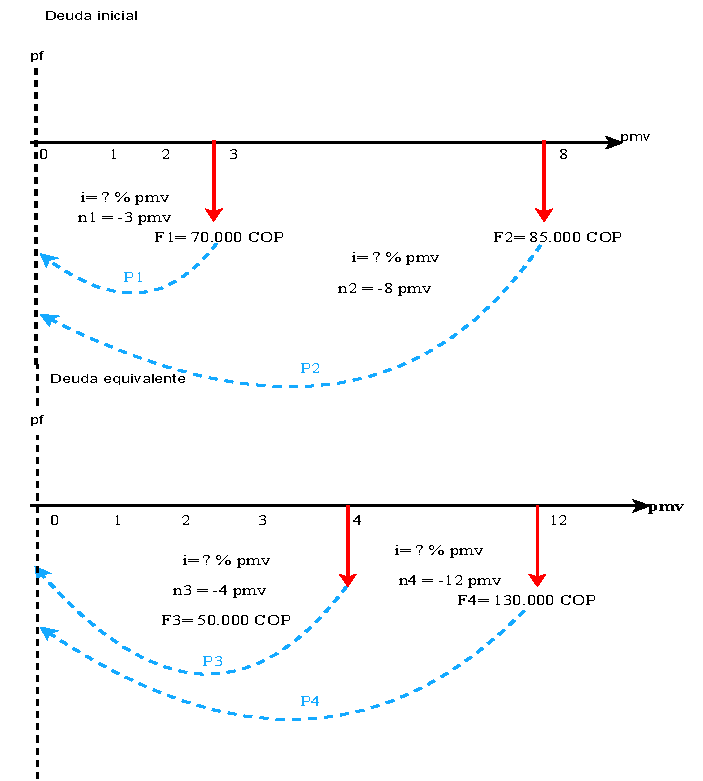
\includegraphics[trim=-5 -5 -5 -5 , scale=0.65]{2_Capitulo/img/ejemplos/14/Ejemplo 14Ver.pdf} } 
    \ \\ \hline
    %%%%%%%%%%%%% FIN INSERCIÓN DE IMAGEN
    %%%%%FIN FLUJO DE CAJA



    %%%%% INICIO DECLARACIÓN FORMULAS
    %%%%%%%%%%% INICIO TITULO
    \rowcolor[HTML]{FFB183}
    \multicolumn{3}{|c|}{\cellcolor[HTML]{FFB183}\textbf{4. Declaración de fórmulas}}                                                       \\ \hline
    %%%%%%%%%%% FIN TITULO
    %%%%%%%%%%% INICIO MATEMÁTICAS

    \multicolumn{3}{|c|}{$P = F(1+i)^{-n} \hspace{0.3cm} \textit{Valor presente }$}                                                         \\
    \multicolumn{3}{|c|}{$P_{1} + P_{2} = P_{3} + P_{4} \hspace{0.3cm} \textit{Ecuación de eqv.}$ }                                         \\
    \hline
    %%%%%%%%%% FIN MATEMÁTICAS
    %%%%%% INICIO DESARROLLO MATEMÁTICO
    \rowcolor[HTML]{FFB183}
    %%%%%%%%%%INICIO TITULO
    \multicolumn{3}{|c|}{\cellcolor[HTML]{FFB183}\textbf{5. Desarrollo matemático}}                                                         \\ \hline
    %%%%%%%%%% FIN TITULO
    %%%%%%%%%% INICIO MATEMÁTICAS


    \multicolumn{3}{|c|}{$ 70.000$ COP $(1+i)^{-3}  + 85.000$ COP $(1+i)^{-8}$}
    \\
    \multicolumn{3}{|c|}{$=50.000$ COP $(1+i)^{-4} + 130.000$ COP $(1+i)^{-12}$}      \\
    \multicolumn{3}{|c|}{$ 70(1+i)^{-3} +85(1+i)^{-8} - 50(1+i)^{-4} - 130(1+i)^{-12} = 0   $ }                                             \\
    \multicolumn{3}{|c|}{$ \textit{Primer ensayo:} $ }                                                                                      \\
    \multicolumn{3}{|c|}{$ i_{1} = 2\% \textit{ pmv} $ }                                                                                    \\
    \multicolumn{3}{|c|}{$70$ COP $(1+0,02)^{-3} +85$ COP $(1+0,02)^{-8}$} 
    \\
    \multicolumn{3}{|c|} {$-50$ COP $(1+0,02)^{-4} - 130$  COP $(1+0,02)^{-12} = -10.18714 $ } \\
    \multicolumn{3}{|c|}{$ \textit{Segundo ensayo:} $ }                                                                                     \\
    \multicolumn{3}{|c|}{$ i_{2} = 3\% \textit{ pmv} $ }                                                                                    \\
    \multicolumn{3}{|c|}{$ 70$ COP $(1+0,03)^{-3} +85$ COP $(1+0,03)^{-8}$}
    \\
    \multicolumn{3}{|c|}{$-50$ COP $(1+0,03)^{-4} -130$ COP $(1+0,03)^{-12} = -4,44404 $ }   \\
    \multicolumn{3}{|c|}{$ \textit{Tercer ensayo:} $ }                                                                                      \\
    \multicolumn{3}{|c|}{$ i_{3} = 4\% \textit{ pmv} $ }                                                                                    \\
    \multicolumn{3}{|c|}{$70$ COP $(1+0,04)^{-3} +85$ COP $(1+0,04)^{-8}$}
    \\
    \multicolumn{3}{|c|}{$-50$ COP $(1+0,04)^{-4} -130$ COP $(1+0,04)^{-12} = 0.400587 $ }
    \\
    
    \multicolumn{3}{|c|}{$ 	\textit{ Se toman los resultados correspondientes al 3\% y a 4\% por ser los más cercanos y} $ }                 \\
    \multicolumn{3}{|c|}{$ 	\textit{los que presentan diferente signo y los colocaremos de la siguiente forma:} $ }                          \\
    \multicolumn{3}{|c|}{$ \textit{ Se plantea una proporción, teniendo en cuenta las diferencias mostradas en los} $ }                     \\
    \multicolumn{3}{|c|}{$ \textit{corchetes y siempre manteniendo el mismo orden.} $ }                                                     \\
    \multicolumn{3}{|c|}{$ \frac{3-i}{3-4} = \frac{-4,44404-0}{-4,44404-0,400587}$ }                                                                \\ \hline


    %%%%%%%%%% FIN MATEMÁTICAS
    %%%%%% FIN DESARROLLO MATEMÁTICO
    %%%%%% INICIO RESPUESTA
    \rowcolor[HTML]{FFB183}
    %%%%%%%%%%INICIO TITULO
    \multicolumn{3}{|c|}{\cellcolor[HTML]{FFB183}\textbf{6. Respuesta}}                                                                     \\ \hline
    %%%%%%%%%% FIN TITULO
    %%%%%%%%%% INICIO RESPUESTA MATEMÁTICA
    \multicolumn{3}{|c|}{

      \begin{minipage}[t][0.07\textheight][c]{0.8\columnwidth}
       \centering
        $i = 3,917313\% \textit{ pmv}$ .
      \end{minipage}
    }                                                                                                                                       \\ \hline


    %%%%%%%%%% FIN MATEMÁTICAS
    %%%%%% FIN RESPUESTA
  \end{longtable}
  %Se crean dos lineas en blanco para que no quede el siguiente texto tan pegado
  %\newline \newline %USARLO SI CREES QUE ES NECESARIO
\end{center}
%%%%%%%%%%%%%%%%%%%%%%%%%%FIN EJERCICIO 14 %%%%%%%%%%%%%%%%%%%%%%%%%%%
%%%%%%%%%%%%%%%%%%%% EJERCICIO 15 %%%%%%

\textbf{Ejemplo 15}\\
Una persona debe pagar  COP  100,000 con vencimiento en 3 meses,  COP  150,000 a 10 meses y
COP  200,000 con vencimiento en un año. Si hace un pago único de  COP  450,000, hallar la fecha en
que debe hacerse, suponga una tasa del 18\% nominal anual mes vencido.
Si consideramos la período focal (pf) en el período mes vencido 12:\\ \\

%\newpage %USAR SOLO SI EL SOLUCIÓN QUEDA SOLO Y ES NECESARIO BAJARLO A LA SIGUIENTE PAGINA
\textbf{Solución.}\\
%La tabla ira centrada
\begin{center}
  \renewcommand{\arraystretch}{1.5}% Margenes de las celdas
  %Creación de la cuadricula de 3 columnas
  \begin{longtable}[H]{|c|c|c|}
    %Creamos una linea horizontal
    \hline
    %Definimos el color de la primera fila
    \rowcolor[HTML]{FFB183}
    %%%%% INICIO ASIGNACIÓN PERíODO FOCAL %%%%%%%
    %%%%%%%%%% INICIO TITULO
    %Lo que se hace aquí es mezclar las 3 columnas en una sola
    \multicolumn{3}{|c|}{\cellcolor[HTML]{FFB183}\textbf{1. Asignación período focal}}                                                                                          \\ \hline
    \multicolumn{3}{|c|}{\textbf{ $pf = \textit{ período focal: 0 pmv} $}}                                                                                                      \\ \hline
    %%%%%%%%%% FIN TITULO
    %%%%% INICIO DECLARACIÓN DE VARIABLES %%%%%%%
    %%%%%%%%%% INICIO TITULO
    %Lo que se hace aquí es mezclar las 3 columnas en una sola
    \multicolumn{3}{|c|}{\cellcolor[HTML]{FFB183}\textbf{2. Declaración de variables}}                                                                                          \\ \hline
    %%%%%%%%%% FIN TITULO
    %%%%%%%%%% INICIO DE MATEMÁTICAS
    %Cada & hace referencia al paso de la siguiente columna

    $j = 18\% \textit{ namv} $                                 & $P_{1} =  COP  100.000  $                                                      & $n_{1} = 9 \textit{ pmv} $    \\
    $i = 1,5\% \textit{ pmv} $                                 & $P_{2} =  COP  150.000  $                                                      & $n_{2} = 2 \textit{ pmv} $    \\
                                                               & $P_{3} =  COP  200.000  $                                                      & $n_{3}= 0 \textit{ pmv}  $    \\
                                                               & $p_{4} =  COP  450.000  $                                                      & $n_{4} = 12-n \textit{ pmv} $ \\ \hline

    %%%%%%%%%% FIN DE MATEMÁTICAS
    %%%%% FIN DECLARACIÓN DE VARIABLES


    %%%%% INICIO FLUJO DE CAJA
    \rowcolor[HTML]{FFB183}
    \multicolumn{3}{|c|}{\cellcolor[HTML]{FFB183}\textbf{3. Diagrama de flujo de caja}}                                                                                         \\ \hline
    %Mezclamos 3 columnas y pondremos el dibujo
    %%%%%%%%%%%%% INSERCIÓN DE LA IMAGEN
    %Deberán descargar las imágenes respectivas del drive y pegarlas en la carpeta
    %n_capitulo/img/ejemplos/1/capitulo1ejemplo1.pdf  (el /1/ es el numero del ejemplo)
    \multicolumn{3}{|c|}{ 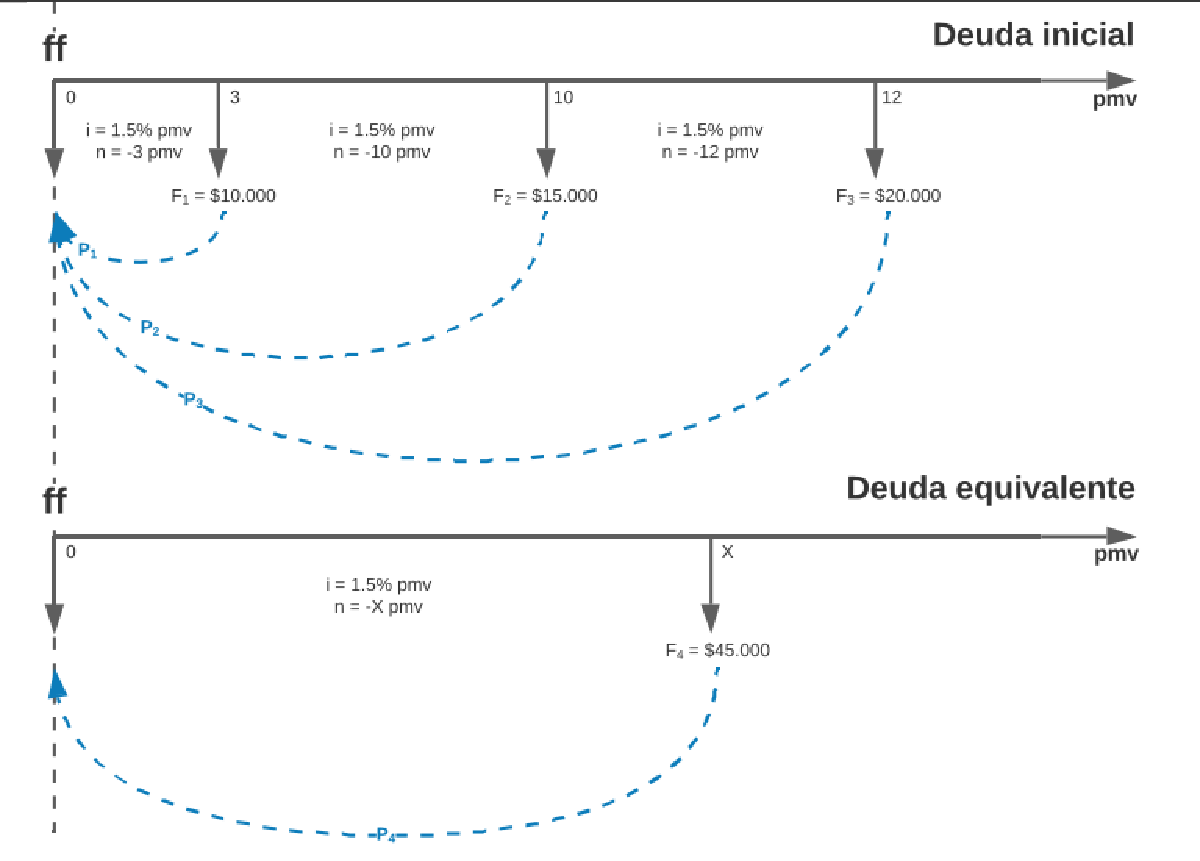
\includegraphics[trim=-5 -5 -5 -5 , scale=0.64]{14/Capitulo2Ejercicio15.pdf} }
    \\ \hline
    %%%%%%%%%%%%% FIN INSERCIÓN DE IMAGEN
    %%%%%FIN FLUJO DE CAJA



    %%%%% INICIO DECLARACIÓN FORMULAS
    %%%%%%%%%%% INICIO TITULO
    \rowcolor[HTML]{FFB183}
    \multicolumn{3}{|c|}{\cellcolor[HTML]{FFB183}\textbf{4. Declaración de fórmulas}}                                                                                           \\ \hline
    %%%%%%%%%%% FIN TITULO
    %%%%%%%%%%% INICIO MATEMÁTICAS

    $P_{1} + P_{2} + P_{3} = P_{4} \textit{ Ecuación de eqv.}$ & \multicolumn{2}{c|}{$P = F(1+i)^(-n) \hspace{0.3cm} \textit{Valor presente}$ }                                 \\
                                                               & \multicolumn{2}{c|}{$F = P(1+i)^n \hspace{0.3cm} \textit{Valor futuro}$   }                                    \\ \hline
    %%%%%%%%%% FIN MATEMÁTICAS
    %%%%%% INICIO DESARROLLO MATEMÁTICO
    \rowcolor[HTML]{FFB183}
    %%%%%%%%%%INICIO TITULO
    \multicolumn{3}{|c|}{\cellcolor[HTML]{FFB183}\textbf{5. Desarrollo matemático}}                                                                                             \\ \hline
    %%%%%%%%%% FIN TITULO
    %%%%%%%%%% INICIO MATEMÁTICAS

    \multicolumn{3}{|C{\linewidth}|}{$  COP  100.000( 1 + 0,015)^(-3) +  COP  150.000( 1 + 0,015)^(-10) +  COP  200.000( 1 + 0,015)^(-12)= COP  450.000( 1 + 0,015)^(-x) $}     \\
    \multicolumn{3}{|C{\linewidth}|}{$ ln(306.090,07391/450.000)= (-x)ln(1,015)  $ }                                                                                            \\ \hline


    %%%%%%%%%% FIN MATEMÁTICAS
    %%%%%% FIN DESARROLLO MATEMÁTICO
    %%%%%% INICIO RESPUESTA
    \rowcolor[HTML]{FFB183}
    %%%%%%%%%%INICIO TITULO
    \multicolumn{3}{|c|}{\cellcolor[HTML]{FFB183}\textbf{6. Respuesta}}                                                                                                         \\ \hline
    %%%%%%%%%% FIN TITULO
    %%%%%%%%%% INICIO RESPUESTA MATEMÁTICA
    \multicolumn{3}{|c|}{

      \begin{minipage}[t][0.07\textheight][c]{0.8\columnwidth}
        $n_{4} = 9,24059 \textit{ pmv} \approx t = 9 \textit{ meses y }  7 \textit{ dias.} $
      \end{minipage}
    }                                                                                                                                                                           \\ \hline


    %%%%%%%%%% FIN MATEMÁTICAS
    %%%%%% FIN RESPUESTA
  \end{longtable}
  %Se crean dos lineas en blanco para que no quede el siguiente texto tan pegado
  %\newline \newline %USARLO SI CREES QUE ES NECESARIO
\end{center}
%%%%%%%%%%%%%%%%%%%%%%%%%%FIN EJERCICIO 15 %%%%%%%%%%%%%%%%%%%%%%%%%%%

%%%%%%%%%%%%%%%%%%% EJERCICIO 14 %%%%%%

\textbf{Ejemplo 14}\\
Una persona debe pagar 70.000 COP en 3 meses y 85.000 COP en 8 meses; ante la imposibilidad de cancelar las deudas en las fechas previstas le ofrece al acreedor que le cancelara 50.000 COP en 4 meses y 130.000 COP en 12 meses. Si el acreedor acepta esta nueva forma de pago ¿Qué tasa de interés periódica mes vencido estará pagando?.\\ \\
\setlength{\parskip}{-1mm}
%\newpage %USAR SOLO SI EL SOLUCIÓN QUEDA SOLO Y ES NECESARIO BAJARLO A LA SIGUIENTE PAGINA
\textbf{Solución.}
%La tabla ira centrada

\begin{center}
  \renewcommand{\arraystretch}{1.5}% Margenes de las celdas
  %Creación de la cuadricula de 3 columnas
  \begin{longtable}[H]{|c|c|c|}
    %Creamos una linea horizontal
    \hline
    %Definimos el color de la primera fila
    \rowcolor[HTML]{FFB183}
    %%%%% INICIO ASIGNACIÓN PERíODO FOCAL %%%%%%%
    %%%%%%%%%% INICIO TITULO
    %Lo que se hace aquí es mezclar las 3 columnas en una sola
    \multicolumn{3}{|c|}{\cellcolor[HTML]{FFB183}\textbf{1. Asignación período focal}}                                                      \\ \hline
    \multicolumn{3}{|c|}{\textbf{ $pf = \textit{ período focal: 0 pmv} $}}                                                                  \\ \hline
    %%%%%%%%%% FIN TITULO
    %%%%% INICIO DECLARACIÓN DE VARIABLES %%%%%%%
    %%%%%%%%%% INICIO TITULO
    %Lo que se hace aquí es mezclar las 3 columnas en una sola
    \multicolumn{3}{|c|}{\cellcolor[HTML]{FFB183}\textbf{2. Declaración de variables}}                                                      \\ \hline
    %%%%%%%%%% FIN TITULO
    %%%%%%%%%% INICIO DE MATEMÁTICAS
    %Cada & hace referencia al paso de la siguiente columna
    $F_{1} =    70.000  $ COP & $F_{3} =    50.000 $  COP  & $n_ {2} = -8 \textit{ pmv}  $                                                  \\
    $F_{2} =    85.000  $ COP & $F_{4} =    130.000  $ COP & $n_ {3} = -4 \textit{ pmv}   $                                                 \\
    $i = ?\%  $               & $n_{1} = -3 \textit{ pmv}  $ & $n_ {4} = -12 \textit{ pmv}  $                                                 \\ \hline

    %%%%%%%%%% FIN DE MATEMÁTICAS
    %%%%% FIN DECLARACIÓN DE VARIABLES


    %%%%% INICIO FLUJO DE CAJA
    \rowcolor[HTML]{FFB183}
    \multicolumn{3}{|c|}{\cellcolor[HTML]{FFB183}\textbf{3. Diagrama de flujo de caja}}                                                     \\ \hline
    %Mezclamos 3 columnas y pondremos el dibujo
    %%%%%%%%%%%%% INSERCIÓN DE LA IMAGEN
    %Deberán descargar las imágenes respectivas del drive y pegarlas en la carpeta
    %n_capitulo/img/ejemplos/1/capitulo1ejemplo1.pdf  (el /1/ es el numero del ejemplo)
    \multicolumn{3}{|c|}{ 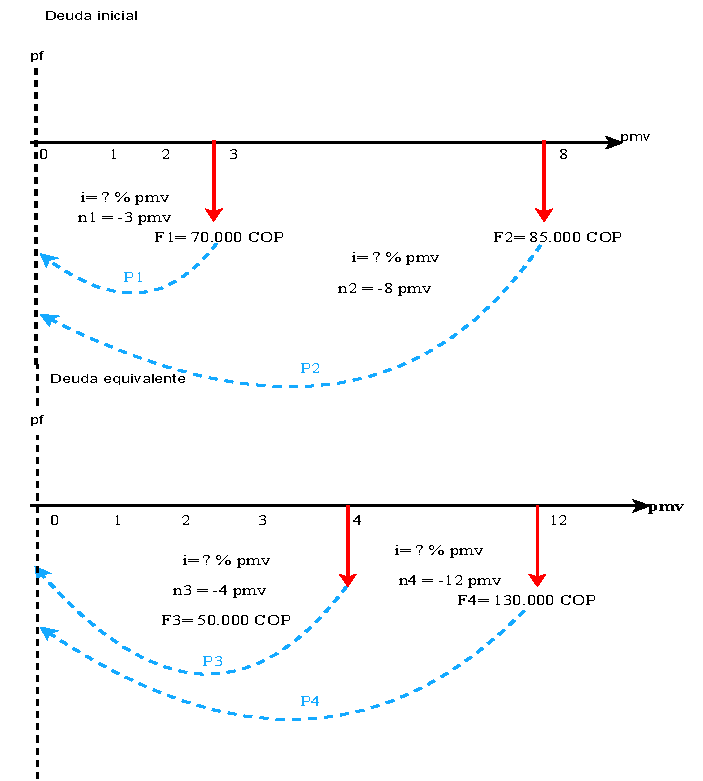
\includegraphics[trim=-5 -5 -5 -5 , scale=0.65]{2_Capitulo/img/ejemplos/14/Ejemplo 14Ver.pdf} } 
    \ \\ \hline
    %%%%%%%%%%%%% FIN INSERCIÓN DE IMAGEN
    %%%%%FIN FLUJO DE CAJA



    %%%%% INICIO DECLARACIÓN FORMULAS
    %%%%%%%%%%% INICIO TITULO
    \rowcolor[HTML]{FFB183}
    \multicolumn{3}{|c|}{\cellcolor[HTML]{FFB183}\textbf{4. Declaración de fórmulas}}                                                       \\ \hline
    %%%%%%%%%%% FIN TITULO
    %%%%%%%%%%% INICIO MATEMÁTICAS

    \multicolumn{3}{|c|}{$P = F(1+i)^{-n} \hspace{0.3cm} \textit{Valor presente }$}                                                         \\
    \multicolumn{3}{|c|}{$P_{1} + P_{2} = P_{3} + P_{4} \hspace{0.3cm} \textit{Ecuación de eqv.}$ }                                         \\
    \hline
    %%%%%%%%%% FIN MATEMÁTICAS
    %%%%%% INICIO DESARROLLO MATEMÁTICO
    \rowcolor[HTML]{FFB183}
    %%%%%%%%%%INICIO TITULO
    \multicolumn{3}{|c|}{\cellcolor[HTML]{FFB183}\textbf{5. Desarrollo matemático}}                                                         \\ \hline
    %%%%%%%%%% FIN TITULO
    %%%%%%%%%% INICIO MATEMÁTICAS


    \multicolumn{3}{|c|}{$ 70.000$ COP $(1+i)^{-3}  + 85.000$ COP $(1+i)^{-8}$}
    \\
    \multicolumn{3}{|c|}{$=50.000$ COP $(1+i)^{-4} + 130.000$ COP $(1+i)^{-12}$}      \\
    \multicolumn{3}{|c|}{$ 70(1+i)^{-3} +85(1+i)^{-8} - 50(1+i)^{-4} - 130(1+i)^{-12} = 0   $ }                                             \\
    \multicolumn{3}{|c|}{$ \textit{Primer ensayo:} $ }                                                                                      \\
    \multicolumn{3}{|c|}{$ i_{1} = 2\% \textit{ pmv} $ }                                                                                    \\
    \multicolumn{3}{|c|}{$70$ COP $(1+0,02)^{-3} +85$ COP $(1+0,02)^{-8}$} 
    \\
    \multicolumn{3}{|c|} {$-50$ COP $(1+0,02)^{-4} - 130$  COP $(1+0,02)^{-12} = -10.18714 $ } \\
    \multicolumn{3}{|c|}{$ \textit{Segundo ensayo:} $ }                                                                                     \\
    \multicolumn{3}{|c|}{$ i_{2} = 3\% \textit{ pmv} $ }                                                                                    \\
    \multicolumn{3}{|c|}{$ 70$ COP $(1+0,03)^{-3} +85$ COP $(1+0,03)^{-8}$}
    \\
    \multicolumn{3}{|c|}{$-50$ COP $(1+0,03)^{-4} -130$ COP $(1+0,03)^{-12} = -4,44404 $ }   \\
    \multicolumn{3}{|c|}{$ \textit{Tercer ensayo:} $ }                                                                                      \\
    \multicolumn{3}{|c|}{$ i_{3} = 4\% \textit{ pmv} $ }                                                                                    \\
    \multicolumn{3}{|c|}{$70$ COP $(1+0,04)^{-3} +85$ COP $(1+0,04)^{-8}$}
    \\
    \multicolumn{3}{|c|}{$-50$ COP $(1+0,04)^{-4} -130$ COP $(1+0,04)^{-12} = 0.400587 $ }
    \\
    
    \multicolumn{3}{|c|}{$ 	\textit{ Se toman los resultados correspondientes al 3\% y a 4\% por ser los más cercanos y} $ }                 \\
    \multicolumn{3}{|c|}{$ 	\textit{los que presentan diferente signo y los colocaremos de la siguiente forma:} $ }                          \\
    \multicolumn{3}{|c|}{$ \textit{ Se plantea una proporción, teniendo en cuenta las diferencias mostradas en los} $ }                     \\
    \multicolumn{3}{|c|}{$ \textit{corchetes y siempre manteniendo el mismo orden.} $ }                                                     \\
    \multicolumn{3}{|c|}{$ \frac{3-i}{3-4} = \frac{-4,44404-0}{-4,44404-0,400587}$ }                                                                \\ \hline


    %%%%%%%%%% FIN MATEMÁTICAS
    %%%%%% FIN DESARROLLO MATEMÁTICO
    %%%%%% INICIO RESPUESTA
    \rowcolor[HTML]{FFB183}
    %%%%%%%%%%INICIO TITULO
    \multicolumn{3}{|c|}{\cellcolor[HTML]{FFB183}\textbf{6. Respuesta}}                                                                     \\ \hline
    %%%%%%%%%% FIN TITULO
    %%%%%%%%%% INICIO RESPUESTA MATEMÁTICA
    \multicolumn{3}{|c|}{

      \begin{minipage}[t][0.07\textheight][c]{0.8\columnwidth}
       \centering
        $i = 3,917313\% \textit{ pmv}$ .
      \end{minipage}
    }                                                                                                                                       \\ \hline


    %%%%%%%%%% FIN MATEMÁTICAS
    %%%%%% FIN RESPUESTA
  \end{longtable}
  %Se crean dos lineas en blanco para que no quede el siguiente texto tan pegado
  %\newline \newline %USARLO SI CREES QUE ES NECESARIO
\end{center}
%%%%%%%%%%%%%%%%%%%%%%%%%%FIN EJERCICIO 14 %%%%%%%%%%%%%%%%%%%%%%%%%%%
